\documentclass[twoside]{book}

% Packages required by doxygen
\usepackage{fixltx2e}
\usepackage{calc}
\usepackage{doxygen}
\usepackage[export]{adjustbox} % also loads graphicx
\usepackage{graphicx}
\usepackage[utf8]{inputenc}
\usepackage{makeidx}
\usepackage{multicol}
\usepackage{multirow}
\PassOptionsToPackage{warn}{textcomp}
\usepackage{textcomp}
\usepackage[nointegrals]{wasysym}
\usepackage[table]{xcolor}

% Font selection
\usepackage[T1]{fontenc}
\usepackage[scaled=.90]{helvet}
\usepackage{courier}
\usepackage{amssymb}
\usepackage{sectsty}
\renewcommand{\familydefault}{\sfdefault}
\allsectionsfont{%
  \fontseries{bc}\selectfont%
  \color{darkgray}%
}
\renewcommand{\DoxyLabelFont}{%
  \fontseries{bc}\selectfont%
  \color{darkgray}%
}
\newcommand{\+}{\discretionary{\mbox{\scriptsize$\hookleftarrow$}}{}{}}

% Page & text layout
\usepackage{geometry}
\geometry{%
  a4paper,%
  top=2.5cm,%
  bottom=2.5cm,%
  left=2.5cm,%
  right=2.5cm%
}
\tolerance=750
\hfuzz=15pt
\hbadness=750
\setlength{\emergencystretch}{15pt}
\setlength{\parindent}{0cm}
\setlength{\parskip}{3ex plus 2ex minus 2ex}
\makeatletter
\renewcommand{\paragraph}{%
  \@startsection{paragraph}{4}{0ex}{-1.0ex}{1.0ex}{%
    \normalfont\normalsize\bfseries\SS@parafont%
  }%
}
\renewcommand{\subparagraph}{%
  \@startsection{subparagraph}{5}{0ex}{-1.0ex}{1.0ex}{%
    \normalfont\normalsize\bfseries\SS@subparafont%
  }%
}
\makeatother

% Headers & footers
\usepackage{fancyhdr}
\pagestyle{fancyplain}
\fancyhead[LE]{\fancyplain{}{\bfseries\thepage}}
\fancyhead[CE]{\fancyplain{}{}}
\fancyhead[RE]{\fancyplain{}{\bfseries\leftmark}}
\fancyhead[LO]{\fancyplain{}{\bfseries\rightmark}}
\fancyhead[CO]{\fancyplain{}{}}
\fancyhead[RO]{\fancyplain{}{\bfseries\thepage}}
\fancyfoot[LE]{\fancyplain{}{}}
\fancyfoot[CE]{\fancyplain{}{}}
\fancyfoot[RE]{\fancyplain{}{\bfseries\scriptsize Generated by Doxygen }}
\fancyfoot[LO]{\fancyplain{}{\bfseries\scriptsize Generated by Doxygen }}
\fancyfoot[CO]{\fancyplain{}{}}
\fancyfoot[RO]{\fancyplain{}{}}
\renewcommand{\footrulewidth}{0.4pt}
\renewcommand{\chaptermark}[1]{%
  \markboth{#1}{}%
}
\renewcommand{\sectionmark}[1]{%
  \markright{\thesection\ #1}%
}

% Indices & bibliography
\usepackage{natbib}
\usepackage[titles]{tocloft}
\setcounter{tocdepth}{3}
\setcounter{secnumdepth}{5}
\makeindex

% Hyperlinks (required, but should be loaded last)
\usepackage{ifpdf}
\ifpdf
  \usepackage[pdftex,pagebackref=true]{hyperref}
\else
  \usepackage[ps2pdf,pagebackref=true]{hyperref}
\fi
\hypersetup{%
  colorlinks=true,%
  linkcolor=blue,%
  citecolor=blue,%
  unicode%
}

% Custom commands
\newcommand{\clearemptydoublepage}{%
  \newpage{\pagestyle{empty}\cleardoublepage}%
}

\usepackage{caption}
\captionsetup{labelsep=space,justification=centering,font={bf},singlelinecheck=off,skip=4pt,position=top}

%===== C O N T E N T S =====

\begin{document}

% Titlepage & ToC
\hypersetup{pageanchor=false,
             bookmarksnumbered=true,
             pdfencoding=unicode
            }
\pagenumbering{alph}
\begin{titlepage}
\vspace*{7cm}
\begin{center}%
{\Large My Project }\\
\vspace*{1cm}
{\large Generated by Doxygen 1.8.14}\\
\end{center}
\end{titlepage}
\clearemptydoublepage
\pagenumbering{roman}
\tableofcontents
\clearemptydoublepage
\pagenumbering{arabic}
\hypersetup{pageanchor=true}

%--- Begin generated contents ---
\chapter{Todo List}
\label{todo}
\Hypertarget{todo}

\begin{DoxyRefList}
\item[\label{todo__todo000003}%
\Hypertarget{todo__todo000003}%
Member \mbox{\hyperlink{classClassSiec_a6f31c5bea93923e8a83e810a1443e9d7}{Class\+Siec\+:\+:add\+\_\+particle}} (double x, double y, double r, double vx=0.\+0, double vy=0.\+0, double max\+Velocity=0.\+0)]max\+Velocity is probably useless  
\item[\label{todo__todo000001}%
\Hypertarget{todo__todo000001}%
Member \mbox{\hyperlink{classClassSiec_a3a1c1350b50c564e85ff7371bff71777}{Class\+Siec\+:\+:Class\+Siec}} (double dt, double box\+\_\+x=800.\+0, double box\+\_\+y=600.\+0)]dt is deprecated  
\item[\label{todo__todo000004}%
\Hypertarget{todo__todo000004}%
Member \mbox{\hyperlink{classClassSiec_aa4c36868471f5747008cea881f1038c1}{Class\+Siec\+:\+:get\+\_\+particle}} (uint64\+\_\+t nr, particle $\ast$here)]Probably useless  
\item[\label{todo__todo000005}%
\Hypertarget{todo__todo000005}%
Member \mbox{\hyperlink{classClassSiec_a87284d96c487a462bf8a42d81fc4bb8c}{Class\+Siec\+:\+:get\+\_\+radial\+\_\+distribution\+\_\+function\+\_\+theoretical}} (void)]Check this  
\item[\label{todo__todo000002}%
\Hypertarget{todo__todo000002}%
Member \mbox{\hyperlink{classClassSiec_a2ef8ae6a08683c8ed1c4e9d89b79e08e}{Class\+Siec\+:\+:set\+\_\+dt}} (double dt)]function is deprecated 
\end{DoxyRefList}
\chapter{Bug List}
\label{bug}
\Hypertarget{bug}

\begin{DoxyRefList}
\item[\label{bug__bug000003}%
\Hypertarget{bug__bug000003}%
Member \mbox{\hyperlink{classClassSiec_a95685407da49bfa4d1a54fd248e8aee3}{Class\+Siec\+:\+:get\+\_\+radial\+\_\+distribution\+\_\+function}} (double r, double dr)]probably bad function  
\item[\label{bug__bug000001}%
\Hypertarget{bug__bug000001}%
Member \mbox{\hyperlink{structparticle_a842a75343ebbcdcaf53e95f0f1286d9a}{particle\+:\+:set\+\_\+max\+Velocity}} (double max\+Velocity)]probably not useful  
\item[\label{bug__bug000002}%
\Hypertarget{bug__bug000002}%
Member \mbox{\hyperlink{structparticle_a4f06bd4316643ca9ba721a4f768763a6}{particle\+:\+:step}} (double dt=1.\+0)]not useful 
\end{DoxyRefList}
\chapter{Class Index}
\section{Class List}
Here are the classes, structs, unions and interfaces with brief descriptions\+:\begin{DoxyCompactList}
\item\contentsline{section}{\mbox{\hyperlink{classClassSiec}{Class\+Siec}} }{\pageref{classClassSiec}}{}
\item\contentsline{section}{\mbox{\hyperlink{structpart__particles}{part\+\_\+particles}} }{\pageref{structpart__particles}}{}
\item\contentsline{section}{\mbox{\hyperlink{structparticle}{particle}} }{\pageref{structparticle}}{}
\item\contentsline{section}{\mbox{\hyperlink{structparticle__zero__time}{particle\+\_\+zero\+\_\+time}} }{\pageref{structparticle__zero__time}}{}
\item\contentsline{section}{\mbox{\hyperlink{structs__pair}{s\+\_\+pair}} }{\pageref{structs__pair}}{}
\end{DoxyCompactList}

\chapter{File Index}
\section{File List}
Here is a list of all files with brief descriptions\+:\begin{DoxyCompactList}
\item\contentsline{section}{\mbox{\hyperlink{ClassSiec_8cpp}{Class\+Siec.\+cpp}} }{\pageref{ClassSiec_8cpp}}{}
\item\contentsline{section}{\mbox{\hyperlink{ClassSiec_8h}{Class\+Siec.\+h}} }{\pageref{ClassSiec_8h}}{}
\item\contentsline{section}{\mbox{\hyperlink{main_8cpp}{main.\+cpp}} }{\pageref{main_8cpp}}{}
\end{DoxyCompactList}

\chapter{Class Documentation}
\hypertarget{classClassSiec}{}\section{Class\+Siec Class Reference}
\label{classClassSiec}\index{Class\+Siec@{Class\+Siec}}


{\ttfamily \#include $<$Class\+Siec.\+h$>$}



Collaboration diagram for Class\+Siec\+:
\nopagebreak
\begin{figure}[H]
\begin{center}
\leavevmode
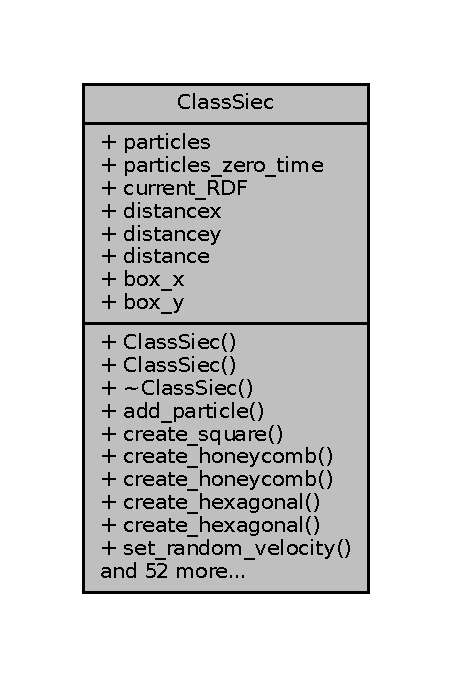
\includegraphics[width=217pt]{classClassSiec__coll__graph}
\end{center}
\end{figure}
\subsection*{Public Member Functions}
\begin{DoxyCompactItemize}
\item 
\mbox{\hyperlink{classClassSiec_ae87ded45ef76f08bf3116f3a933126a1}{Class\+Siec}} (void)
\item 
\mbox{\hyperlink{classClassSiec_a3a1c1350b50c564e85ff7371bff71777}{Class\+Siec}} (double dt, double \mbox{\hyperlink{classClassSiec_a8ebc9e2a0a8f7ccf4736482aa2a5f673}{box\+\_\+x}}=800.\+0, double \mbox{\hyperlink{classClassSiec_a51b98a4d58f22b84e410eaf2c7b31c4b}{box\+\_\+y}}=600.\+0)
\item 
virtual \mbox{\hyperlink{classClassSiec_a0a4837ae00000cb4bc7a1f0deca000b5}{$\sim$\+Class\+Siec}} (void)
\item 
int \mbox{\hyperlink{classClassSiec_a6f31c5bea93923e8a83e810a1443e9d7}{add\+\_\+particle}} (double x, double y, double r, double vx=0.\+0, double vy=0.\+0, double max\+Velocity=0.\+0)
\item 
int \mbox{\hyperlink{classClassSiec_a4b34a96c2302a69832378955e515349c}{create\+\_\+square}} (double a, double r)
\item 
int \mbox{\hyperlink{classClassSiec_a67d2e9b6ac5a7031d153336071fe0b1a}{create\+\_\+honeycomb}} (double a, double r)
\item 
int \mbox{\hyperlink{classClassSiec_a293f258a3a45122d0d59bd6b827f0442}{create\+\_\+honeycomb}} (double a, double r, double density, double precision=0.\+01)
\item 
int \mbox{\hyperlink{classClassSiec_af9d21e3ef4441737d3c64271c5752532}{create\+\_\+hexagonal}} (double a, double r)
\item 
int \mbox{\hyperlink{classClassSiec_a89393fb8f724ede8d628e46018e692a3}{create\+\_\+hexagonal}} (double a, double r, double density, double precision)
\item 
int \mbox{\hyperlink{classClassSiec_a29968ccc2e9318ca89ae0b3dac4a390d}{set\+\_\+random\+\_\+velocity}} (double multiplier=1.\+0)
\item 
int \mbox{\hyperlink{classClassSiec_a4b63c475330f7b0c96a244f55a624fac}{set\+\_\+random\+\_\+size}} (double min, double max)
\item 
int \mbox{\hyperlink{classClassSiec_a361b139e9734e15599847d2060d85d6b}{set\+\_\+mass\+\_\+to\+\_\+radius}} (double ratio=1.\+0)
\item 
int \mbox{\hyperlink{classClassSiec_aa2eff85fe7fc842b2d0631118d533154}{set\+\_\+mass\+\_\+to\+\_\+area}} (double ratio=1.\+0)
\item 
int \mbox{\hyperlink{classClassSiec_a2adaa0e7fe44a2a68b7eba11c52d21bd}{set\+\_\+mass\+\_\+all}} (double mass=1.\+0)
\item 
int \mbox{\hyperlink{classClassSiec_ab2a445e522e2d8c59177fd28c074c1c1}{set\+\_\+momentum\+\_\+to\+\_\+zero}} (double Ekpoz\+\_\+t, double precision=0.\+001)
\item 
int \mbox{\hyperlink{classClassSiec_a37811fccdbeb4119061a02cfb9386677}{set\+\_\+particles\+\_\+zero\+\_\+time}} (void)
\item 
int \mbox{\hyperlink{classClassSiec_a2ef8ae6a08683c8ed1c4e9d89b79e08e}{set\+\_\+dt}} (double dt)
\item 
uint64\+\_\+t \mbox{\hyperlink{classClassSiec_a5fa315d36ce3648e5e5c2bf66b744e18}{get\+\_\+particles\+\_\+len}} (void)
\item 
int \mbox{\hyperlink{classClassSiec_aa4c36868471f5747008cea881f1038c1}{get\+\_\+particle}} (uint64\+\_\+t nr, \mbox{\hyperlink{structparticle}{particle}} $\ast$here)
\item 
\mbox{\hyperlink{structs__pair}{s\+\_\+pair}} \mbox{\hyperlink{classClassSiec_a1f8a44832453567a2eeed85fe038ca01}{get\+\_\+next\+\_\+collision\+\_\+particle\+\_\+number}} (void)
\item 
double \mbox{\hyperlink{classClassSiec_a654072dec38aee93903bdce321890a80}{get\+\_\+next\+\_\+collision\+\_\+particles}} (vector$<$ \mbox{\hyperlink{structs__pair}{s\+\_\+pair}} $>$ $\ast$ptr)
\item 
float \mbox{\hyperlink{classClassSiec_a27ab9475c3e1da5cba2c8dce28e12444}{get\+\_\+time}} (void)
\item 
float \mbox{\hyperlink{classClassSiec_ae0e08ad933601148dcd2edc998c17a61}{get\+\_\+temperature}} (void)
\item 
float \mbox{\hyperlink{classClassSiec_a1ea898d8e6cb52ffc47e7490e48894e4}{get\+\_\+density}} (void)
\item 
float \mbox{\hyperlink{classClassSiec_aad61574e5a2c57c21f3404b7a60ee189}{get\+\_\+density\+\_\+real}} (void)
\item 
float \mbox{\hyperlink{classClassSiec_a1b7f3db9473b2660b3a6c1dfeee45e22}{get\+\_\+packing\+\_\+ratio}} (void)
\item 
double \mbox{\hyperlink{classClassSiec_ae5515f653846b695b3ab00682d15c6fc}{get\+\_\+kinetic\+\_\+energy}} (void)
\item 
uint64\+\_\+t \mbox{\hyperlink{classClassSiec_ac5f8e08337a1ef96531495a6aee8bfb9}{get\+\_\+number\+\_\+of\+\_\+particles\+\_\+in\+\_\+radius}} (double r, double dr, \mbox{\hyperlink{structparticle}{particle}} $\ast$for\+\_\+particle)
\item 
uint64\+\_\+t \mbox{\hyperlink{classClassSiec_a0c89392852117a823a1a603f4181b3a7}{get\+\_\+number\+\_\+of\+\_\+particles\+\_\+in\+\_\+radius}} (double r, double dr)
\item 
float \mbox{\hyperlink{classClassSiec_a1a3c05e29d9fb646f1733704db81933d}{get\+\_\+radial\+\_\+distribution\+\_\+function}} (double r, double dr, \mbox{\hyperlink{structparticle}{particle}} $\ast$for\+\_\+particle, uint64\+\_\+t prec=100)
\item 
float \mbox{\hyperlink{classClassSiec_a95685407da49bfa4d1a54fd248e8aee3}{get\+\_\+radial\+\_\+distribution\+\_\+function}} (double r, double dr)
\item 
float \mbox{\hyperlink{classClassSiec_a87284d96c487a462bf8a42d81fc4bb8c}{get\+\_\+radial\+\_\+distribution\+\_\+function\+\_\+theoretical}} (void)
\item 
float \mbox{\hyperlink{classClassSiec_a8fb2e1fa04229aaa6027fed8dd996aea}{get\+\_\+state\+\_\+space\+\_\+\+Boublik}} (void)
\item 
float \mbox{\hyperlink{classClassSiec_a36144a1734674d3f0c6899c348da1a97}{get\+\_\+state\+\_\+space\+\_\+\+Handerson}} (void)
\item 
float \mbox{\hyperlink{classClassSiec_a3a0171519c3557d8edec22edb5978c9c}{get\+\_\+state\+\_\+space\+\_\+\+Solan}} (void)
\item 
float \mbox{\hyperlink{classClassSiec_acffa9f63d7236490d4e214a59e443140}{get\+\_\+\+Velocity\+\_\+\+Autocorrelation\+\_\+\+Function}} (void)
\item 
float \mbox{\hyperlink{classClassSiec_a59f6ca8740aad85697541a0c9901d699}{get\+\_\+diffusivity}} (void)
\item 
double \mbox{\hyperlink{classClassSiec_a5d81d2e727712fbb0f6f596eee09f354}{get\+\_\+diffusitivity\+\_\+delta}} (void)
\item 
double \mbox{\hyperlink{classClassSiec_a21be4d09c7aa47a5d3f216509ad5feef}{get\+\_\+\+Velocity\+\_\+\+Autocorrelation\+\_\+\+Function\+\_\+delta}} (void)
\item 
double \mbox{\hyperlink{classClassSiec_ac410df30c33bfc1e1613390446e716db}{get\+\_\+diffusitivity\+\_\+delta\+\_\+ratio}} (void)
\item 
double \mbox{\hyperlink{classClassSiec_af6d6dbab3224e645c67e6c7dd2e02378}{get\+\_\+\+Velocity\+\_\+\+Autocorrelation\+\_\+\+Function\+\_\+delta\+\_\+ratio}} (void)
\item 
double \mbox{\hyperlink{classClassSiec_a44e57165a1c37b9f9073fa0334e2878d}{get\+\_\+box\+\_\+x}} (void)
\item 
double \mbox{\hyperlink{classClassSiec_a6670e040d5bd507051671b8bd856c7d0}{get\+\_\+box\+\_\+y}} (void)
\item 
double \mbox{\hyperlink{classClassSiec_ab17d2e44f433cb4aec5d965b158a60a1}{get\+\_\+min\+\_\+radius}} (void)
\item 
double \mbox{\hyperlink{classClassSiec_a078c088fe48696423cc5c6c429d45eab}{get\+\_\+max\+\_\+radius}} (void)
\item 
void \mbox{\hyperlink{classClassSiec_ab883e160c0a8878ce20b8a27fea9b65f}{convert\+\_\+to\+\_\+box}} (double $\ast$x, double $\ast$y)
\item 
std\+::string \mbox{\hyperlink{classClassSiec_a5228f0e683612ae0a947f77a2bb7d2c9}{get\+\_\+box\+\_\+info}} (std\+::string sep=\char`\"{}\textbackslash{})
\item 
std\+::string \mbox{\hyperlink{classClassSiec_a653414664f006ee8cbfb8d101c8e8e62}{get\+\_\+box\+\_\+info\+\_\+title}} (std\+::string sep=\char`\"{}\textbackslash{})
\item 
std\+::string \mbox{\hyperlink{classClassSiec_a1e4fd45f66e131050359072b706f7608}{get\+\_\+box\+\_\+info\+\_\+raw}} (std\+::string sep=\char`\"{}\textbackslash{})
\item 
std\+::string \mbox{\hyperlink{classClassSiec_a609cc786246741388e18ed50c0165388}{get\+\_\+\+R\+D\+F\+\_\+r}} (double r, double dr, uint64\+\_\+t prec=100, std\+::string sep=\char`\"{} \char`\"{})
\item 
std\+::string \mbox{\hyperlink{classClassSiec_aad7c55f1dfa1b5bca25fc39e0b509304}{get\+\_\+\+R\+D\+F\+\_\+r}} (uint64\+\_\+t prec=100, std\+::string sep=\char`\"{} \char`\"{})
\item 
std\+::string \mbox{\hyperlink{classClassSiec_aaf3b24bc73d268f151acdff6351214e0}{get\+\_\+static\+\_\+parameters\+\_\+info}} (std\+::string sep=\char`\"{}\textbackslash{})
\item 
std\+::string \mbox{\hyperlink{classClassSiec_a1fcb70fc39cb91fe5b5382c7911de316}{get\+\_\+static\+\_\+parameters\+\_\+title}} (std\+::string sep=\char`\"{}\textbackslash{})
\item 
std\+::string \mbox{\hyperlink{classClassSiec_abed8d28e81524a99ab325569db15bb36}{get\+\_\+static\+\_\+parameters\+\_\+raw}} (std\+::string sep=\char`\"{}\textbackslash{})
\item 
int \mbox{\hyperlink{classClassSiec_a984c7c1d77c9cf78b6254529088028a4}{save\+\_\+\+R\+DF}} (uint64\+\_\+t prec=100, std\+::string sep=\char`\"{} \char`\"{})
\item 
void \mbox{\hyperlink{classClassSiec_a9c96b5d39e27f8f2bdda6fd60113ceb6}{save\+\_\+\+R\+D\+F\+\_\+to\+\_\+array}} (vector$<$ double $>$ $\ast$array, uint64\+\_\+t prec=100)
\item 
int \mbox{\hyperlink{classClassSiec_a4527492cd521a36e1bcad1cb38034784}{fix\+\_\+position}} (void)
\item 
int \mbox{\hyperlink{classClassSiec_a5c2c133544d66df25e8b13e6b710272e}{init}} (std\+::string filename)
\item 
int \mbox{\hyperlink{classClassSiec_ab49b9f6b28f5e3c319384f518042272a}{insert\+\_\+to\+\_\+file}} (std\+::string data)
\item 
int \mbox{\hyperlink{classClassSiec_aa6e0a35a8b5387e43ee4f518ee101d74}{flush\+\_\+file}} (void)
\item 
int \mbox{\hyperlink{classClassSiec_aa0f4586cbe65a86ba011772287a546a9}{close\+\_\+file}} (void)
\item 
int \mbox{\hyperlink{classClassSiec_a0de17762248441c53936ee7924776052}{step\+\_\+all}} (int debug=0)
\end{DoxyCompactItemize}
\subsection*{Public Attributes}
\begin{DoxyCompactItemize}
\item 
vector$<$ \mbox{\hyperlink{structparticle}{particle}} $>$ \mbox{\hyperlink{classClassSiec_aa1a11eee47b10c11930952f092110e94}{particles}}
\item 
vector$<$ \mbox{\hyperlink{structparticle__zero__time}{particle\+\_\+zero\+\_\+time}} $>$ \mbox{\hyperlink{classClassSiec_aa1096135e230dbae78ec05efc8a4725f}{particles\+\_\+zero\+\_\+time}}
\item 
vector$<$ double $>$ \mbox{\hyperlink{classClassSiec_aaa4641c3eb550d26c64a785729e8cd63}{current\+\_\+\+R\+DF}}
\item 
double \mbox{\hyperlink{classClassSiec_a98e9ee22a2e12ce6612d1ce6e785cda2}{distancex}}
\item 
double \mbox{\hyperlink{classClassSiec_a5c100f779c613f9c747b0b7a3f02f2d9}{distancey}}
\item 
double \mbox{\hyperlink{classClassSiec_a4593ac900fa92dd33f9b40010b35efb9}{distance}}
\item 
double \mbox{\hyperlink{classClassSiec_a8ebc9e2a0a8f7ccf4736482aa2a5f673}{box\+\_\+x}}
\item 
double \mbox{\hyperlink{classClassSiec_a51b98a4d58f22b84e410eaf2c7b31c4b}{box\+\_\+y}}
\end{DoxyCompactItemize}


\subsection{Detailed Description}


Definition at line 105 of file Class\+Siec.\+h.



\subsection{Constructor \& Destructor Documentation}
\mbox{\Hypertarget{classClassSiec_ae87ded45ef76f08bf3116f3a933126a1}\label{classClassSiec_ae87ded45ef76f08bf3116f3a933126a1}} 
\index{Class\+Siec@{Class\+Siec}!Class\+Siec@{Class\+Siec}}
\index{Class\+Siec@{Class\+Siec}!Class\+Siec@{Class\+Siec}}
\subsubsection{\texorpdfstring{Class\+Siec()}{ClassSiec()}\hspace{0.1cm}{\footnotesize\ttfamily [1/2]}}
{\footnotesize\ttfamily Class\+Siec\+::\+Class\+Siec (\begin{DoxyParamCaption}\item[{void}]{ }\end{DoxyParamCaption})}



Definition at line 354 of file Class\+Siec.\+cpp.



References box\+\_\+x, and box\+\_\+y.

\mbox{\Hypertarget{classClassSiec_a3a1c1350b50c564e85ff7371bff71777}\label{classClassSiec_a3a1c1350b50c564e85ff7371bff71777}} 
\index{Class\+Siec@{Class\+Siec}!Class\+Siec@{Class\+Siec}}
\index{Class\+Siec@{Class\+Siec}!Class\+Siec@{Class\+Siec}}
\subsubsection{\texorpdfstring{Class\+Siec()}{ClassSiec()}\hspace{0.1cm}{\footnotesize\ttfamily [2/2]}}
{\footnotesize\ttfamily Class\+Siec\+::\+Class\+Siec (\begin{DoxyParamCaption}\item[{double}]{dt,  }\item[{double}]{box\+\_\+x = {\ttfamily 800.0},  }\item[{double}]{box\+\_\+y = {\ttfamily 600.0} }\end{DoxyParamCaption})}

Constructor \begin{DoxyRefDesc}{Todo}
\item[\mbox{\hyperlink{todo__todo000001}{Todo}}]dt is deprecated \end{DoxyRefDesc}

\begin{DoxyParams}{Parameters}
{\em dt} & -\/$>$ deprecated \\
\hline
{\em box\+\_\+x} & \\
\hline
{\em box\+\_\+y} & \\
\hline
\end{DoxyParams}


Definition at line 372 of file Class\+Siec.\+cpp.



References box\+\_\+x, and box\+\_\+y.

\mbox{\Hypertarget{classClassSiec_a0a4837ae00000cb4bc7a1f0deca000b5}\label{classClassSiec_a0a4837ae00000cb4bc7a1f0deca000b5}} 
\index{Class\+Siec@{Class\+Siec}!````~Class\+Siec@{$\sim$\+Class\+Siec}}
\index{````~Class\+Siec@{$\sim$\+Class\+Siec}!Class\+Siec@{Class\+Siec}}
\subsubsection{\texorpdfstring{$\sim$\+Class\+Siec()}{~ClassSiec()}}
{\footnotesize\ttfamily Class\+Siec\+::$\sim$\+Class\+Siec (\begin{DoxyParamCaption}\item[{void}]{ }\end{DoxyParamCaption})\hspace{0.3cm}{\ttfamily [virtual]}}



Definition at line 383 of file Class\+Siec.\+cpp.



References particles.



\subsection{Member Function Documentation}
\mbox{\Hypertarget{classClassSiec_a6f31c5bea93923e8a83e810a1443e9d7}\label{classClassSiec_a6f31c5bea93923e8a83e810a1443e9d7}} 
\index{Class\+Siec@{Class\+Siec}!add\+\_\+particle@{add\+\_\+particle}}
\index{add\+\_\+particle@{add\+\_\+particle}!Class\+Siec@{Class\+Siec}}
\subsubsection{\texorpdfstring{add\+\_\+particle()}{add\_particle()}}
{\footnotesize\ttfamily int Class\+Siec\+::add\+\_\+particle (\begin{DoxyParamCaption}\item[{double}]{x,  }\item[{double}]{y,  }\item[{double}]{r,  }\item[{double}]{vx = {\ttfamily 0.0},  }\item[{double}]{vy = {\ttfamily 0.0},  }\item[{double}]{max\+Velocity = {\ttfamily 0.0} }\end{DoxyParamCaption})}

Add particle to array \begin{DoxyRefDesc}{Todo}
\item[\mbox{\hyperlink{todo__todo000003}{Todo}}]max\+Velocity is probably useless \end{DoxyRefDesc}

\begin{DoxyParams}{Parameters}
{\em x} & \\
\hline
{\em y} & \\
\hline
{\em r} & \\
\hline
{\em vx} & \\
\hline
{\em vy} & \\
\hline
{\em max\+Velocity} & \\
\hline
\end{DoxyParams}
\begin{DoxyReturn}{Returns}

\end{DoxyReturn}


Definition at line 432 of file Class\+Siec.\+cpp.



References OK, and particles.



Referenced by create\+\_\+hexagonal(), create\+\_\+honeycomb(), and create\+\_\+square().

\mbox{\Hypertarget{classClassSiec_aa0f4586cbe65a86ba011772287a546a9}\label{classClassSiec_aa0f4586cbe65a86ba011772287a546a9}} 
\index{Class\+Siec@{Class\+Siec}!close\+\_\+file@{close\+\_\+file}}
\index{close\+\_\+file@{close\+\_\+file}!Class\+Siec@{Class\+Siec}}
\subsubsection{\texorpdfstring{close\+\_\+file()}{close\_file()}}
{\footnotesize\ttfamily int Class\+Siec\+::close\+\_\+file (\begin{DoxyParamCaption}\item[{void}]{ }\end{DoxyParamCaption})}

Flush and close file \begin{DoxyReturn}{Returns}

\end{DoxyReturn}


Definition at line 990 of file Class\+Siec.\+cpp.



References OK.



Referenced by main().

\mbox{\Hypertarget{classClassSiec_ab883e160c0a8878ce20b8a27fea9b65f}\label{classClassSiec_ab883e160c0a8878ce20b8a27fea9b65f}} 
\index{Class\+Siec@{Class\+Siec}!convert\+\_\+to\+\_\+box@{convert\+\_\+to\+\_\+box}}
\index{convert\+\_\+to\+\_\+box@{convert\+\_\+to\+\_\+box}!Class\+Siec@{Class\+Siec}}
\subsubsection{\texorpdfstring{convert\+\_\+to\+\_\+box()}{convert\_to\_box()}}
{\footnotesize\ttfamily void Class\+Siec\+::convert\+\_\+to\+\_\+box (\begin{DoxyParamCaption}\item[{double $\ast$}]{x,  }\item[{double $\ast$}]{y }\end{DoxyParamCaption})}

Set positions to box 
\begin{DoxyParams}{Parameters}
{\em x} & \\
\hline
{\em y} & \\
\hline
\end{DoxyParams}


Definition at line 405 of file Class\+Siec.\+cpp.



References box\+\_\+x, and box\+\_\+y.

\mbox{\Hypertarget{classClassSiec_af9d21e3ef4441737d3c64271c5752532}\label{classClassSiec_af9d21e3ef4441737d3c64271c5752532}} 
\index{Class\+Siec@{Class\+Siec}!create\+\_\+hexagonal@{create\+\_\+hexagonal}}
\index{create\+\_\+hexagonal@{create\+\_\+hexagonal}!Class\+Siec@{Class\+Siec}}
\subsubsection{\texorpdfstring{create\+\_\+hexagonal()}{create\_hexagonal()}\hspace{0.1cm}{\footnotesize\ttfamily [1/2]}}
{\footnotesize\ttfamily int Class\+Siec\+::create\+\_\+hexagonal (\begin{DoxyParamCaption}\item[{double}]{a,  }\item[{double}]{r }\end{DoxyParamCaption})}

Adds particles in the form of a hexagonal 
\begin{DoxyParams}{Parameters}
{\em a} & \\
\hline
{\em r} & \\
\hline
\end{DoxyParams}
\begin{DoxyReturn}{Returns}

\end{DoxyReturn}


Definition at line 632 of file Class\+Siec.\+cpp.



References add\+\_\+particle(), box\+\_\+x, box\+\_\+y, and OK.

Here is the call graph for this function\+:\nopagebreak
\begin{figure}[H]
\begin{center}
\leavevmode
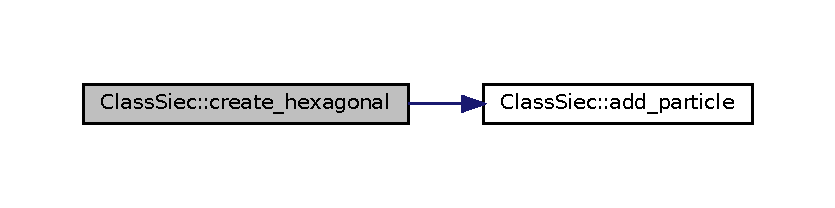
\includegraphics[width=350pt]{classClassSiec_af9d21e3ef4441737d3c64271c5752532_cgraph}
\end{center}
\end{figure}
\mbox{\Hypertarget{classClassSiec_a89393fb8f724ede8d628e46018e692a3}\label{classClassSiec_a89393fb8f724ede8d628e46018e692a3}} 
\index{Class\+Siec@{Class\+Siec}!create\+\_\+hexagonal@{create\+\_\+hexagonal}}
\index{create\+\_\+hexagonal@{create\+\_\+hexagonal}!Class\+Siec@{Class\+Siec}}
\subsubsection{\texorpdfstring{create\+\_\+hexagonal()}{create\_hexagonal()}\hspace{0.1cm}{\footnotesize\ttfamily [2/2]}}
{\footnotesize\ttfamily int Class\+Siec\+::create\+\_\+hexagonal (\begin{DoxyParamCaption}\item[{double}]{a,  }\item[{double}]{r,  }\item[{double}]{density,  }\item[{double}]{precision }\end{DoxyParamCaption})}

Generate hexagonal lattice with desired density 
\begin{DoxyParams}{Parameters}
{\em a} & \\
\hline
{\em r} & \\
\hline
{\em density} & \\
\hline
{\em precision} & \\
\hline
\end{DoxyParams}
\begin{DoxyReturn}{Returns}

\end{DoxyReturn}


Definition at line 576 of file Class\+Siec.\+cpp.



References add\+\_\+particle(), box\+\_\+x, box\+\_\+y, find\+\_\+is\+\_\+in\+\_\+range(), get\+\_\+density\+\_\+real(), OK, and particles.

Here is the call graph for this function\+:\nopagebreak
\begin{figure}[H]
\begin{center}
\leavevmode
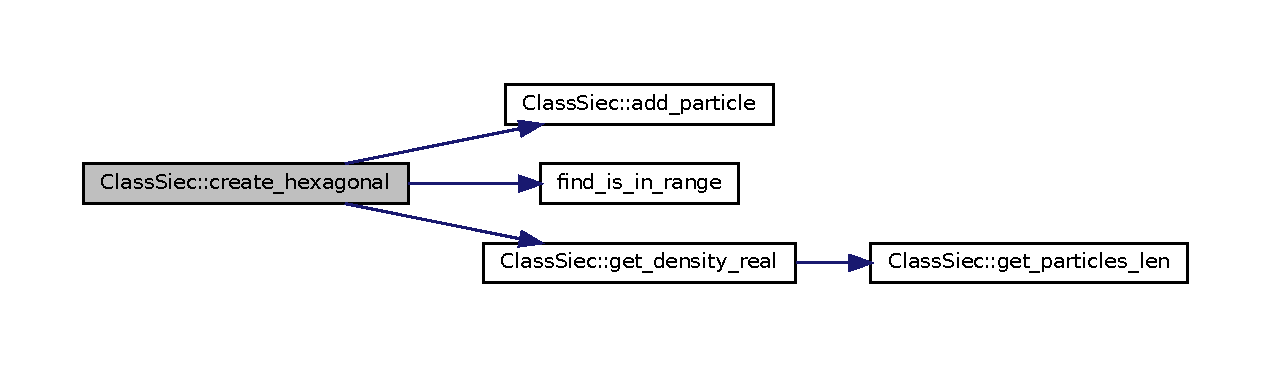
\includegraphics[width=350pt]{classClassSiec_a89393fb8f724ede8d628e46018e692a3_cgraph}
\end{center}
\end{figure}
\mbox{\Hypertarget{classClassSiec_a67d2e9b6ac5a7031d153336071fe0b1a}\label{classClassSiec_a67d2e9b6ac5a7031d153336071fe0b1a}} 
\index{Class\+Siec@{Class\+Siec}!create\+\_\+honeycomb@{create\+\_\+honeycomb}}
\index{create\+\_\+honeycomb@{create\+\_\+honeycomb}!Class\+Siec@{Class\+Siec}}
\subsubsection{\texorpdfstring{create\+\_\+honeycomb()}{create\_honeycomb()}\hspace{0.1cm}{\footnotesize\ttfamily [1/2]}}
{\footnotesize\ttfamily int Class\+Siec\+::create\+\_\+honeycomb (\begin{DoxyParamCaption}\item[{double}]{a,  }\item[{double}]{r }\end{DoxyParamCaption})}

Adds particles in the form of a honeycomb 
\begin{DoxyParams}{Parameters}
{\em a} & \\
\hline
{\em r} & \\
\hline
\end{DoxyParams}
\begin{DoxyReturn}{Returns}

\end{DoxyReturn}


Definition at line 477 of file Class\+Siec.\+cpp.



References add\+\_\+particle(), box\+\_\+x, box\+\_\+y, and OK.



Referenced by main().

Here is the call graph for this function\+:\nopagebreak
\begin{figure}[H]
\begin{center}
\leavevmode
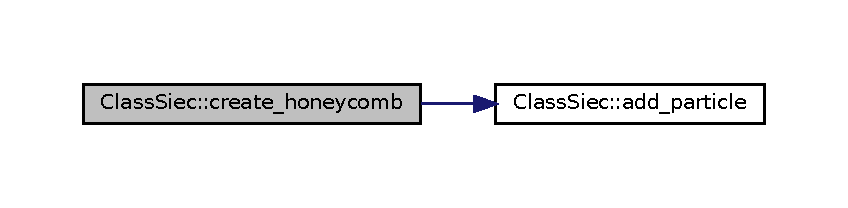
\includegraphics[width=350pt]{classClassSiec_a67d2e9b6ac5a7031d153336071fe0b1a_cgraph}
\end{center}
\end{figure}
\mbox{\Hypertarget{classClassSiec_a293f258a3a45122d0d59bd6b827f0442}\label{classClassSiec_a293f258a3a45122d0d59bd6b827f0442}} 
\index{Class\+Siec@{Class\+Siec}!create\+\_\+honeycomb@{create\+\_\+honeycomb}}
\index{create\+\_\+honeycomb@{create\+\_\+honeycomb}!Class\+Siec@{Class\+Siec}}
\subsubsection{\texorpdfstring{create\+\_\+honeycomb()}{create\_honeycomb()}\hspace{0.1cm}{\footnotesize\ttfamily [2/2]}}
{\footnotesize\ttfamily int Class\+Siec\+::create\+\_\+honeycomb (\begin{DoxyParamCaption}\item[{double}]{a,  }\item[{double}]{r,  }\item[{double}]{density,  }\item[{double}]{precision = {\ttfamily 0.01} }\end{DoxyParamCaption})}

Generate honeycomb lattice with desired density 
\begin{DoxyParams}{Parameters}
{\em a} & \\
\hline
{\em r} & \\
\hline
{\em density} & \\
\hline
{\em precision} & \\
\hline
\end{DoxyParams}
\begin{DoxyReturn}{Returns}

\end{DoxyReturn}


Definition at line 514 of file Class\+Siec.\+cpp.



References add\+\_\+particle(), box\+\_\+x, box\+\_\+y, find\+\_\+is\+\_\+in\+\_\+range(), get\+\_\+density\+\_\+real(), OK, and particles.

Here is the call graph for this function\+:
\nopagebreak
\begin{figure}[H]
\begin{center}
\leavevmode
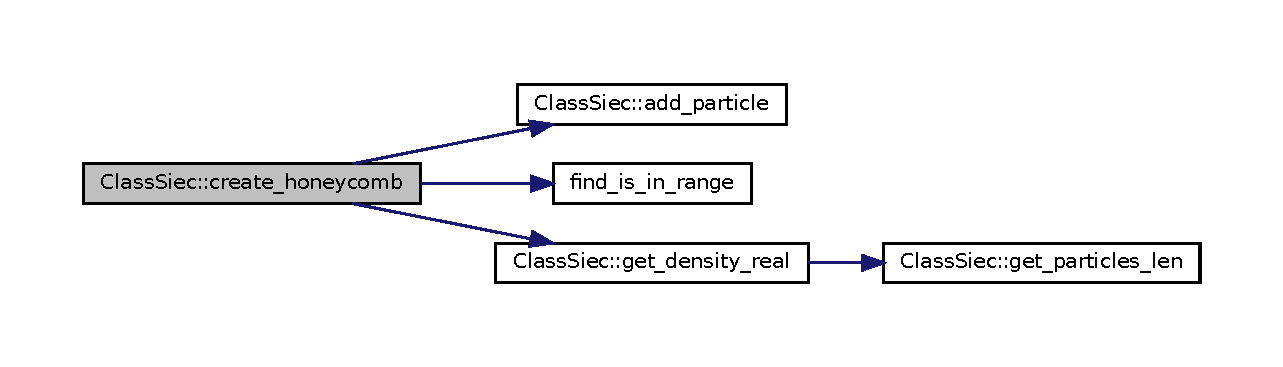
\includegraphics[width=350pt]{classClassSiec_a293f258a3a45122d0d59bd6b827f0442_cgraph}
\end{center}
\end{figure}
\mbox{\Hypertarget{classClassSiec_a4b34a96c2302a69832378955e515349c}\label{classClassSiec_a4b34a96c2302a69832378955e515349c}} 
\index{Class\+Siec@{Class\+Siec}!create\+\_\+square@{create\+\_\+square}}
\index{create\+\_\+square@{create\+\_\+square}!Class\+Siec@{Class\+Siec}}
\subsubsection{\texorpdfstring{create\+\_\+square()}{create\_square()}}
{\footnotesize\ttfamily int Class\+Siec\+::create\+\_\+square (\begin{DoxyParamCaption}\item[{double}]{a,  }\item[{double}]{r }\end{DoxyParamCaption})}

Adds particles in the form of a square 
\begin{DoxyParams}{Parameters}
{\em a} & \\
\hline
{\em r} & \\
\hline
\end{DoxyParams}
\begin{DoxyReturn}{Returns}

\end{DoxyReturn}


Definition at line 448 of file Class\+Siec.\+cpp.



References add\+\_\+particle(), box\+\_\+x, box\+\_\+y, and OK.

Here is the call graph for this function\+:\nopagebreak
\begin{figure}[H]
\begin{center}
\leavevmode
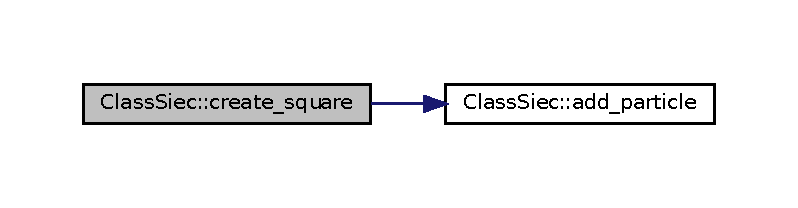
\includegraphics[width=350pt]{classClassSiec_a4b34a96c2302a69832378955e515349c_cgraph}
\end{center}
\end{figure}
\mbox{\Hypertarget{classClassSiec_a4527492cd521a36e1bcad1cb38034784}\label{classClassSiec_a4527492cd521a36e1bcad1cb38034784}} 
\index{Class\+Siec@{Class\+Siec}!fix\+\_\+position@{fix\+\_\+position}}
\index{fix\+\_\+position@{fix\+\_\+position}!Class\+Siec@{Class\+Siec}}
\subsubsection{\texorpdfstring{fix\+\_\+position()}{fix\_position()}}
{\footnotesize\ttfamily int Class\+Siec\+::fix\+\_\+position (\begin{DoxyParamCaption}\item[{void}]{ }\end{DoxyParamCaption})}

Repair positions of all particles to the box \begin{DoxyReturn}{Returns}

\end{DoxyReturn}


Definition at line 936 of file Class\+Siec.\+cpp.



References box\+\_\+x, box\+\_\+y, get\+\_\+particles\+\_\+len(), OK, particles, and th\+\_\+to\+\_\+box().



Referenced by main(), and step\+\_\+all().

Here is the call graph for this function\+:\nopagebreak
\begin{figure}[H]
\begin{center}
\leavevmode
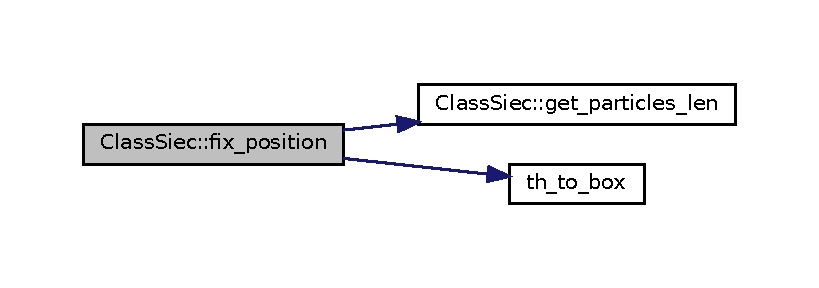
\includegraphics[width=350pt]{classClassSiec_a4527492cd521a36e1bcad1cb38034784_cgraph}
\end{center}
\end{figure}
\mbox{\Hypertarget{classClassSiec_aa6e0a35a8b5387e43ee4f518ee101d74}\label{classClassSiec_aa6e0a35a8b5387e43ee4f518ee101d74}} 
\index{Class\+Siec@{Class\+Siec}!flush\+\_\+file@{flush\+\_\+file}}
\index{flush\+\_\+file@{flush\+\_\+file}!Class\+Siec@{Class\+Siec}}
\subsubsection{\texorpdfstring{flush\+\_\+file()}{flush\_file()}}
{\footnotesize\ttfamily int Class\+Siec\+::flush\+\_\+file (\begin{DoxyParamCaption}\item[{void}]{ }\end{DoxyParamCaption})}



Definition at line 979 of file Class\+Siec.\+cpp.



References OK.



Referenced by main(), and thread\+\_\+siec().

\mbox{\Hypertarget{classClassSiec_a5228f0e683612ae0a947f77a2bb7d2c9}\label{classClassSiec_a5228f0e683612ae0a947f77a2bb7d2c9}} 
\index{Class\+Siec@{Class\+Siec}!get\+\_\+box\+\_\+info@{get\+\_\+box\+\_\+info}}
\index{get\+\_\+box\+\_\+info@{get\+\_\+box\+\_\+info}!Class\+Siec@{Class\+Siec}}
\subsubsection{\texorpdfstring{get\+\_\+box\+\_\+info()}{get\_box\_info()}}
{\footnotesize\ttfamily std\+::string Class\+Siec\+::get\+\_\+box\+\_\+info (\begin{DoxyParamCaption}\item[{std\+::string}]{sep = {\ttfamily \char`\"{}\textbackslash{}t\char`\"{}} }\end{DoxyParamCaption})}

Get box info -\/$>$ info for save in logs \begin{DoxyReturn}{Returns}

\end{DoxyReturn}


Definition at line 1511 of file Class\+Siec.\+cpp.



References get\+\_\+diffusitivity\+\_\+delta(), get\+\_\+diffusivity(), get\+\_\+\+Velocity\+\_\+\+Autocorrelation\+\_\+\+Function(), and get\+\_\+\+Velocity\+\_\+\+Autocorrelation\+\_\+\+Function\+\_\+delta().



Referenced by step\+\_\+all().

Here is the call graph for this function\+:\nopagebreak
\begin{figure}[H]
\begin{center}
\leavevmode
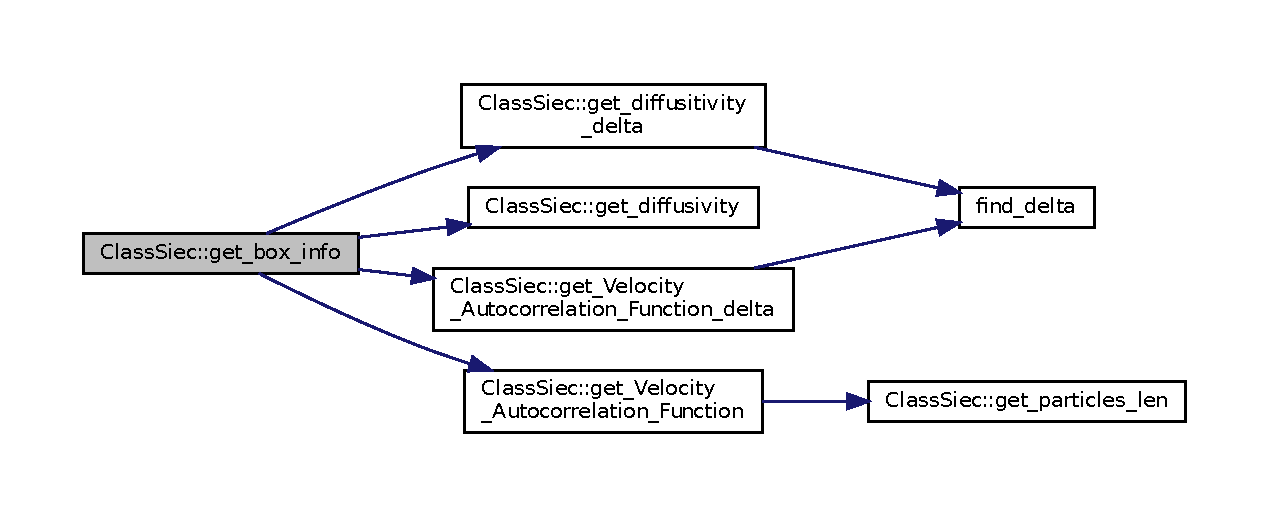
\includegraphics[width=350pt]{classClassSiec_a5228f0e683612ae0a947f77a2bb7d2c9_cgraph}
\end{center}
\end{figure}
\mbox{\Hypertarget{classClassSiec_a1e4fd45f66e131050359072b706f7608}\label{classClassSiec_a1e4fd45f66e131050359072b706f7608}} 
\index{Class\+Siec@{Class\+Siec}!get\+\_\+box\+\_\+info\+\_\+raw@{get\+\_\+box\+\_\+info\+\_\+raw}}
\index{get\+\_\+box\+\_\+info\+\_\+raw@{get\+\_\+box\+\_\+info\+\_\+raw}!Class\+Siec@{Class\+Siec}}
\subsubsection{\texorpdfstring{get\+\_\+box\+\_\+info\+\_\+raw()}{get\_box\_info\_raw()}}
{\footnotesize\ttfamily std\+::string Class\+Siec\+::get\+\_\+box\+\_\+info\+\_\+raw (\begin{DoxyParamCaption}\item[{std\+::string}]{sep = {\ttfamily \char`\"{}\textbackslash{}t\char`\"{}} }\end{DoxyParamCaption})}

Get raw data of info 
\begin{DoxyParams}{Parameters}
{\em sep} & \\
\hline
\end{DoxyParams}
\begin{DoxyReturn}{Returns}

\end{DoxyReturn}


Definition at line 1585 of file Class\+Siec.\+cpp.



References get\+\_\+diffusitivity\+\_\+delta(), get\+\_\+diffusivity(), get\+\_\+\+Velocity\+\_\+\+Autocorrelation\+\_\+\+Function(), and get\+\_\+\+Velocity\+\_\+\+Autocorrelation\+\_\+\+Function\+\_\+delta().



Referenced by step\+\_\+all().

Here is the call graph for this function\+:\nopagebreak
\begin{figure}[H]
\begin{center}
\leavevmode
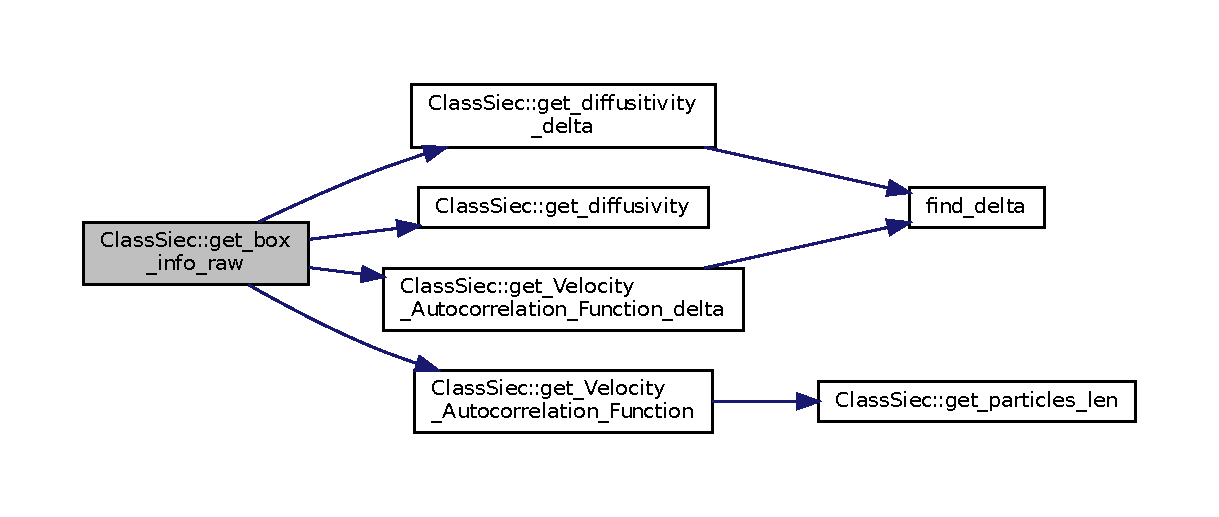
\includegraphics[width=350pt]{classClassSiec_a1e4fd45f66e131050359072b706f7608_cgraph}
\end{center}
\end{figure}
\mbox{\Hypertarget{classClassSiec_a653414664f006ee8cbfb8d101c8e8e62}\label{classClassSiec_a653414664f006ee8cbfb8d101c8e8e62}} 
\index{Class\+Siec@{Class\+Siec}!get\+\_\+box\+\_\+info\+\_\+title@{get\+\_\+box\+\_\+info\+\_\+title}}
\index{get\+\_\+box\+\_\+info\+\_\+title@{get\+\_\+box\+\_\+info\+\_\+title}!Class\+Siec@{Class\+Siec}}
\subsubsection{\texorpdfstring{get\+\_\+box\+\_\+info\+\_\+title()}{get\_box\_info\_title()}}
{\footnotesize\ttfamily std\+::string Class\+Siec\+::get\+\_\+box\+\_\+info\+\_\+title (\begin{DoxyParamCaption}\item[{std\+::string}]{sep = {\ttfamily \char`\"{}\textbackslash{}t\char`\"{}} }\end{DoxyParamCaption})}

Return title of infos 
\begin{DoxyParams}{Parameters}
{\em sep} & \\
\hline
\end{DoxyParams}
\begin{DoxyReturn}{Returns}

\end{DoxyReturn}


Definition at line 1548 of file Class\+Siec.\+cpp.



Referenced by init().

\mbox{\Hypertarget{classClassSiec_a44e57165a1c37b9f9073fa0334e2878d}\label{classClassSiec_a44e57165a1c37b9f9073fa0334e2878d}} 
\index{Class\+Siec@{Class\+Siec}!get\+\_\+box\+\_\+x@{get\+\_\+box\+\_\+x}}
\index{get\+\_\+box\+\_\+x@{get\+\_\+box\+\_\+x}!Class\+Siec@{Class\+Siec}}
\subsubsection{\texorpdfstring{get\+\_\+box\+\_\+x()}{get\_box\_x()}}
{\footnotesize\ttfamily double Class\+Siec\+::get\+\_\+box\+\_\+x (\begin{DoxyParamCaption}\item[{void}]{ }\end{DoxyParamCaption})}



Definition at line 1454 of file Class\+Siec.\+cpp.



References box\+\_\+x.



Referenced by draw\+\_\+all().

\mbox{\Hypertarget{classClassSiec_a6670e040d5bd507051671b8bd856c7d0}\label{classClassSiec_a6670e040d5bd507051671b8bd856c7d0}} 
\index{Class\+Siec@{Class\+Siec}!get\+\_\+box\+\_\+y@{get\+\_\+box\+\_\+y}}
\index{get\+\_\+box\+\_\+y@{get\+\_\+box\+\_\+y}!Class\+Siec@{Class\+Siec}}
\subsubsection{\texorpdfstring{get\+\_\+box\+\_\+y()}{get\_box\_y()}}
{\footnotesize\ttfamily double Class\+Siec\+::get\+\_\+box\+\_\+y (\begin{DoxyParamCaption}\item[{void}]{ }\end{DoxyParamCaption})}



Definition at line 1458 of file Class\+Siec.\+cpp.



References box\+\_\+y.



Referenced by draw\+\_\+all().

\mbox{\Hypertarget{classClassSiec_a1ea898d8e6cb52ffc47e7490e48894e4}\label{classClassSiec_a1ea898d8e6cb52ffc47e7490e48894e4}} 
\index{Class\+Siec@{Class\+Siec}!get\+\_\+density@{get\+\_\+density}}
\index{get\+\_\+density@{get\+\_\+density}!Class\+Siec@{Class\+Siec}}
\subsubsection{\texorpdfstring{get\+\_\+density()}{get\_density()}}
{\footnotesize\ttfamily float Class\+Siec\+::get\+\_\+density (\begin{DoxyParamCaption}\item[{void}]{ }\end{DoxyParamCaption})}

Get density particles in box \begin{DoxyReturn}{Returns}

\end{DoxyReturn}


Definition at line 1161 of file Class\+Siec.\+cpp.



References box\+\_\+x, box\+\_\+y, and get\+\_\+particles\+\_\+len().



Referenced by get\+\_\+radial\+\_\+distribution\+\_\+function(), get\+\_\+\+R\+D\+F\+\_\+r(), get\+\_\+state\+\_\+space\+\_\+\+Boublik(), get\+\_\+state\+\_\+space\+\_\+\+Handerson(), get\+\_\+state\+\_\+space\+\_\+\+Solan(), get\+\_\+static\+\_\+parameters\+\_\+info(), get\+\_\+static\+\_\+parameters\+\_\+raw(), and thread\+\_\+\+R\+D\+F().

Here is the call graph for this function\+:\nopagebreak
\begin{figure}[H]
\begin{center}
\leavevmode
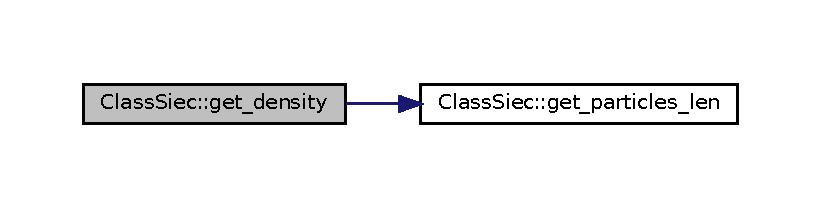
\includegraphics[width=350pt]{classClassSiec_a1ea898d8e6cb52ffc47e7490e48894e4_cgraph}
\end{center}
\end{figure}
\mbox{\Hypertarget{classClassSiec_aad61574e5a2c57c21f3404b7a60ee189}\label{classClassSiec_aad61574e5a2c57c21f3404b7a60ee189}} 
\index{Class\+Siec@{Class\+Siec}!get\+\_\+density\+\_\+real@{get\+\_\+density\+\_\+real}}
\index{get\+\_\+density\+\_\+real@{get\+\_\+density\+\_\+real}!Class\+Siec@{Class\+Siec}}
\subsubsection{\texorpdfstring{get\+\_\+density\+\_\+real()}{get\_density\_real()}}
{\footnotesize\ttfamily float Class\+Siec\+::get\+\_\+density\+\_\+real (\begin{DoxyParamCaption}\item[{void}]{ }\end{DoxyParamCaption})}

Get density(real) particles in box \begin{DoxyReturn}{Returns}

\end{DoxyReturn}


Definition at line 1179 of file Class\+Siec.\+cpp.



References box\+\_\+x, box\+\_\+y, get\+\_\+particles\+\_\+len(), and particles.



Referenced by create\+\_\+hexagonal(), create\+\_\+honeycomb(), get\+\_\+static\+\_\+parameters\+\_\+info(), and get\+\_\+static\+\_\+parameters\+\_\+raw().

Here is the call graph for this function\+:\nopagebreak
\begin{figure}[H]
\begin{center}
\leavevmode
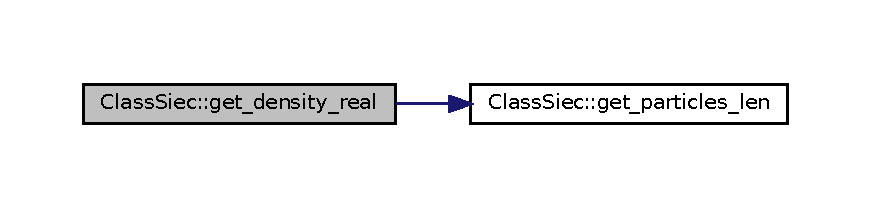
\includegraphics[width=350pt]{classClassSiec_aad61574e5a2c57c21f3404b7a60ee189_cgraph}
\end{center}
\end{figure}
\mbox{\Hypertarget{classClassSiec_a5d81d2e727712fbb0f6f596eee09f354}\label{classClassSiec_a5d81d2e727712fbb0f6f596eee09f354}} 
\index{Class\+Siec@{Class\+Siec}!get\+\_\+diffusitivity\+\_\+delta@{get\+\_\+diffusitivity\+\_\+delta}}
\index{get\+\_\+diffusitivity\+\_\+delta@{get\+\_\+diffusitivity\+\_\+delta}!Class\+Siec@{Class\+Siec}}
\subsubsection{\texorpdfstring{get\+\_\+diffusitivity\+\_\+delta()}{get\_diffusitivity\_delta()}}
{\footnotesize\ttfamily double Class\+Siec\+::get\+\_\+diffusitivity\+\_\+delta (\begin{DoxyParamCaption}\item[{void}]{ }\end{DoxyParamCaption})}

Get diffusivity delta \begin{DoxyReturn}{Returns}

\end{DoxyReturn}


Definition at line 1426 of file Class\+Siec.\+cpp.



References find\+\_\+delta().



Referenced by get\+\_\+box\+\_\+info(), get\+\_\+box\+\_\+info\+\_\+raw(), get\+\_\+static\+\_\+parameters\+\_\+info(), get\+\_\+static\+\_\+parameters\+\_\+raw(), and thread\+\_\+siec().

Here is the call graph for this function\+:\nopagebreak
\begin{figure}[H]
\begin{center}
\leavevmode
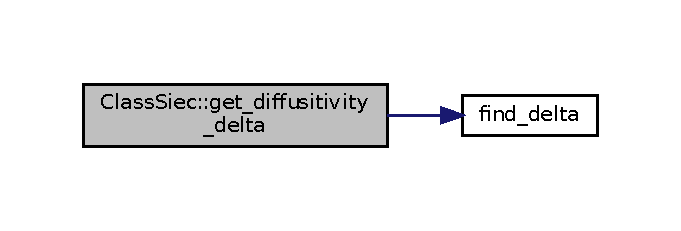
\includegraphics[width=327pt]{classClassSiec_a5d81d2e727712fbb0f6f596eee09f354_cgraph}
\end{center}
\end{figure}
\mbox{\Hypertarget{classClassSiec_ac410df30c33bfc1e1613390446e716db}\label{classClassSiec_ac410df30c33bfc1e1613390446e716db}} 
\index{Class\+Siec@{Class\+Siec}!get\+\_\+diffusitivity\+\_\+delta\+\_\+ratio@{get\+\_\+diffusitivity\+\_\+delta\+\_\+ratio}}
\index{get\+\_\+diffusitivity\+\_\+delta\+\_\+ratio@{get\+\_\+diffusitivity\+\_\+delta\+\_\+ratio}!Class\+Siec@{Class\+Siec}}
\subsubsection{\texorpdfstring{get\+\_\+diffusitivity\+\_\+delta\+\_\+ratio()}{get\_diffusitivity\_delta\_ratio()}}
{\footnotesize\ttfamily double Class\+Siec\+::get\+\_\+diffusitivity\+\_\+delta\+\_\+ratio (\begin{DoxyParamCaption}\item[{void}]{ }\end{DoxyParamCaption})}

Get diffusivity delta ratio \begin{DoxyReturn}{Returns}

\end{DoxyReturn}


Definition at line 1440 of file Class\+Siec.\+cpp.



References find\+\_\+delta(), and get\+\_\+diffusivity().



Referenced by get\+\_\+static\+\_\+parameters\+\_\+info(), and get\+\_\+static\+\_\+parameters\+\_\+raw().

Here is the call graph for this function\+:\nopagebreak
\begin{figure}[H]
\begin{center}
\leavevmode
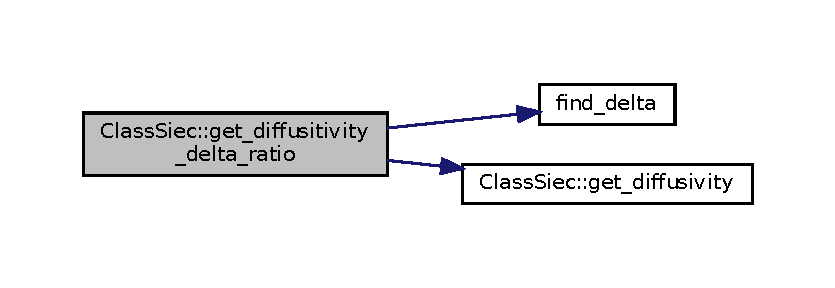
\includegraphics[width=350pt]{classClassSiec_ac410df30c33bfc1e1613390446e716db_cgraph}
\end{center}
\end{figure}
\mbox{\Hypertarget{classClassSiec_a59f6ca8740aad85697541a0c9901d699}\label{classClassSiec_a59f6ca8740aad85697541a0c9901d699}} 
\index{Class\+Siec@{Class\+Siec}!get\+\_\+diffusivity@{get\+\_\+diffusivity}}
\index{get\+\_\+diffusivity@{get\+\_\+diffusivity}!Class\+Siec@{Class\+Siec}}
\subsubsection{\texorpdfstring{get\+\_\+diffusivity()}{get\_diffusivity()}}
{\footnotesize\ttfamily float Class\+Siec\+::get\+\_\+diffusivity (\begin{DoxyParamCaption}\item[{void}]{ }\end{DoxyParamCaption})}

Get diffusivity \begin{DoxyReturn}{Returns}

\end{DoxyReturn}


Definition at line 1417 of file Class\+Siec.\+cpp.



Referenced by get\+\_\+box\+\_\+info(), get\+\_\+box\+\_\+info\+\_\+raw(), get\+\_\+diffusitivity\+\_\+delta\+\_\+ratio(), get\+\_\+static\+\_\+parameters\+\_\+info(), and get\+\_\+static\+\_\+parameters\+\_\+raw().

\mbox{\Hypertarget{classClassSiec_ae5515f653846b695b3ab00682d15c6fc}\label{classClassSiec_ae5515f653846b695b3ab00682d15c6fc}} 
\index{Class\+Siec@{Class\+Siec}!get\+\_\+kinetic\+\_\+energy@{get\+\_\+kinetic\+\_\+energy}}
\index{get\+\_\+kinetic\+\_\+energy@{get\+\_\+kinetic\+\_\+energy}!Class\+Siec@{Class\+Siec}}
\subsubsection{\texorpdfstring{get\+\_\+kinetic\+\_\+energy()}{get\_kinetic\_energy()}}
{\footnotesize\ttfamily double Class\+Siec\+::get\+\_\+kinetic\+\_\+energy (\begin{DoxyParamCaption}\item[{void}]{ }\end{DoxyParamCaption})}

Get the kinetic energy of particles \begin{DoxyReturn}{Returns}

\end{DoxyReturn}


Definition at line 1217 of file Class\+Siec.\+cpp.



References get\+\_\+particles\+\_\+len(), and particles.



Referenced by set\+\_\+momentum\+\_\+to\+\_\+zero().

Here is the call graph for this function\+:\nopagebreak
\begin{figure}[H]
\begin{center}
\leavevmode
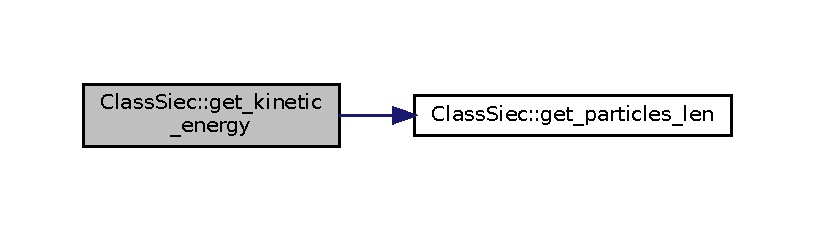
\includegraphics[width=350pt]{classClassSiec_ae5515f653846b695b3ab00682d15c6fc_cgraph}
\end{center}
\end{figure}
\mbox{\Hypertarget{classClassSiec_a078c088fe48696423cc5c6c429d45eab}\label{classClassSiec_a078c088fe48696423cc5c6c429d45eab}} 
\index{Class\+Siec@{Class\+Siec}!get\+\_\+max\+\_\+radius@{get\+\_\+max\+\_\+radius}}
\index{get\+\_\+max\+\_\+radius@{get\+\_\+max\+\_\+radius}!Class\+Siec@{Class\+Siec}}
\subsubsection{\texorpdfstring{get\+\_\+max\+\_\+radius()}{get\_max\_radius()}}
{\footnotesize\ttfamily double Class\+Siec\+::get\+\_\+max\+\_\+radius (\begin{DoxyParamCaption}\item[{void}]{ }\end{DoxyParamCaption})}



Definition at line 1477 of file Class\+Siec.\+cpp.



References get\+\_\+particles\+\_\+len(), and particles.

Here is the call graph for this function\+:
\nopagebreak
\begin{figure}[H]
\begin{center}
\leavevmode
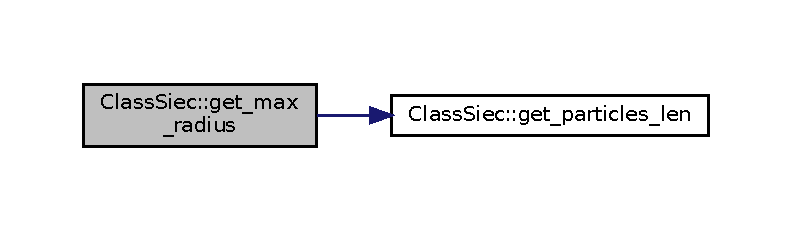
\includegraphics[width=350pt]{classClassSiec_a078c088fe48696423cc5c6c429d45eab_cgraph}
\end{center}
\end{figure}
\mbox{\Hypertarget{classClassSiec_ab17d2e44f433cb4aec5d965b158a60a1}\label{classClassSiec_ab17d2e44f433cb4aec5d965b158a60a1}} 
\index{Class\+Siec@{Class\+Siec}!get\+\_\+min\+\_\+radius@{get\+\_\+min\+\_\+radius}}
\index{get\+\_\+min\+\_\+radius@{get\+\_\+min\+\_\+radius}!Class\+Siec@{Class\+Siec}}
\subsubsection{\texorpdfstring{get\+\_\+min\+\_\+radius()}{get\_min\_radius()}}
{\footnotesize\ttfamily double Class\+Siec\+::get\+\_\+min\+\_\+radius (\begin{DoxyParamCaption}\item[{void}]{ }\end{DoxyParamCaption})}



Definition at line 1463 of file Class\+Siec.\+cpp.



References get\+\_\+particles\+\_\+len(), and particles.



Referenced by main(), step\+\_\+all(), and thread\+\_\+\+R\+D\+F().

Here is the call graph for this function\+:
\nopagebreak
\begin{figure}[H]
\begin{center}
\leavevmode
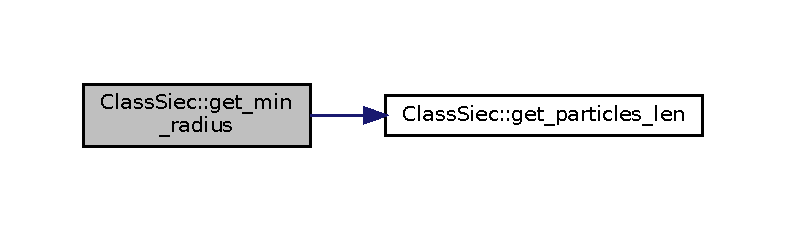
\includegraphics[width=350pt]{classClassSiec_ab17d2e44f433cb4aec5d965b158a60a1_cgraph}
\end{center}
\end{figure}
\mbox{\Hypertarget{classClassSiec_a1f8a44832453567a2eeed85fe038ca01}\label{classClassSiec_a1f8a44832453567a2eeed85fe038ca01}} 
\index{Class\+Siec@{Class\+Siec}!get\+\_\+next\+\_\+collision\+\_\+particle\+\_\+number@{get\+\_\+next\+\_\+collision\+\_\+particle\+\_\+number}}
\index{get\+\_\+next\+\_\+collision\+\_\+particle\+\_\+number@{get\+\_\+next\+\_\+collision\+\_\+particle\+\_\+number}!Class\+Siec@{Class\+Siec}}
\subsubsection{\texorpdfstring{get\+\_\+next\+\_\+collision\+\_\+particle\+\_\+number()}{get\_next\_collision\_particle\_number()}}
{\footnotesize\ttfamily \mbox{\hyperlink{structs__pair}{s\+\_\+pair}} Class\+Siec\+::get\+\_\+next\+\_\+collision\+\_\+particle\+\_\+number (\begin{DoxyParamCaption}\item[{void}]{ }\end{DoxyParamCaption})}

Return pair of next collision \begin{DoxyReturn}{Returns}

\end{DoxyReturn}


Definition at line 861 of file Class\+Siec.\+cpp.



References box\+\_\+x, box\+\_\+y, get\+\_\+particles\+\_\+len(), and particles.

Here is the call graph for this function\+:
\nopagebreak
\begin{figure}[H]
\begin{center}
\leavevmode
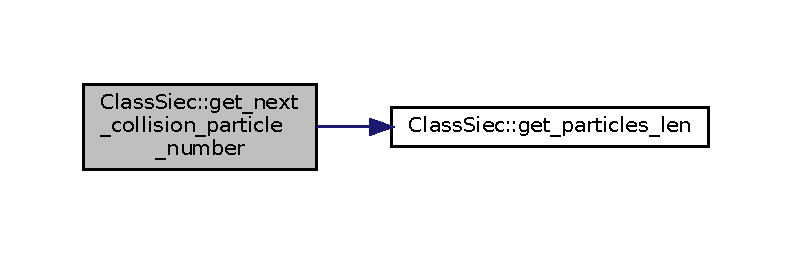
\includegraphics[width=350pt]{classClassSiec_a1f8a44832453567a2eeed85fe038ca01_cgraph}
\end{center}
\end{figure}
\mbox{\Hypertarget{classClassSiec_a654072dec38aee93903bdce321890a80}\label{classClassSiec_a654072dec38aee93903bdce321890a80}} 
\index{Class\+Siec@{Class\+Siec}!get\+\_\+next\+\_\+collision\+\_\+particles@{get\+\_\+next\+\_\+collision\+\_\+particles}}
\index{get\+\_\+next\+\_\+collision\+\_\+particles@{get\+\_\+next\+\_\+collision\+\_\+particles}!Class\+Siec@{Class\+Siec}}
\subsubsection{\texorpdfstring{get\+\_\+next\+\_\+collision\+\_\+particles()}{get\_next\_collision\_particles()}}
{\footnotesize\ttfamily double Class\+Siec\+::get\+\_\+next\+\_\+collision\+\_\+particles (\begin{DoxyParamCaption}\item[{vector$<$ \mbox{\hyperlink{structs__pair}{s\+\_\+pair}} $>$ $\ast$}]{pairs }\end{DoxyParamCaption})}

Fills the tables of the next collisions 
\begin{DoxyParams}{Parameters}
{\em pairs} & \\
\hline
\end{DoxyParams}
\begin{DoxyReturn}{Returns}

\end{DoxyReturn}


Definition at line 893 of file Class\+Siec.\+cpp.



References box\+\_\+x, box\+\_\+y, get\+\_\+particles\+\_\+len(), and particles.



Referenced by step\+\_\+all().

Here is the call graph for this function\+:
\nopagebreak
\begin{figure}[H]
\begin{center}
\leavevmode
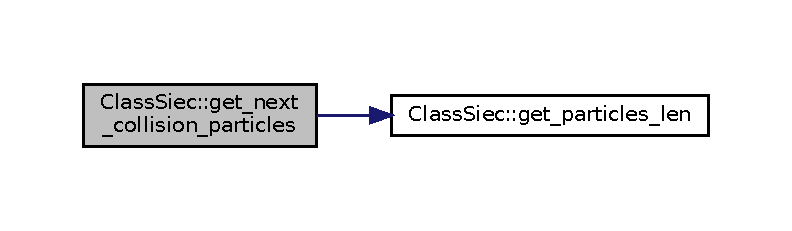
\includegraphics[width=350pt]{classClassSiec_a654072dec38aee93903bdce321890a80_cgraph}
\end{center}
\end{figure}
\mbox{\Hypertarget{classClassSiec_ac5f8e08337a1ef96531495a6aee8bfb9}\label{classClassSiec_ac5f8e08337a1ef96531495a6aee8bfb9}} 
\index{Class\+Siec@{Class\+Siec}!get\+\_\+number\+\_\+of\+\_\+particles\+\_\+in\+\_\+radius@{get\+\_\+number\+\_\+of\+\_\+particles\+\_\+in\+\_\+radius}}
\index{get\+\_\+number\+\_\+of\+\_\+particles\+\_\+in\+\_\+radius@{get\+\_\+number\+\_\+of\+\_\+particles\+\_\+in\+\_\+radius}!Class\+Siec@{Class\+Siec}}
\subsubsection{\texorpdfstring{get\+\_\+number\+\_\+of\+\_\+particles\+\_\+in\+\_\+radius()}{get\_number\_of\_particles\_in\_radius()}\hspace{0.1cm}{\footnotesize\ttfamily [1/2]}}
{\footnotesize\ttfamily uint64\+\_\+t Class\+Siec\+::get\+\_\+number\+\_\+of\+\_\+particles\+\_\+in\+\_\+radius (\begin{DoxyParamCaption}\item[{double}]{r,  }\item[{double}]{dr,  }\item[{\mbox{\hyperlink{structparticle}{particle}} $\ast$}]{for\+\_\+particle }\end{DoxyParamCaption})}

Get the number of particles in radius for center of particle 
\begin{DoxyParams}{Parameters}
{\em r} & \\
\hline
{\em dr} & \\
\hline
{\em for\+\_\+particle} & \\
\hline
\end{DoxyParams}
\begin{DoxyReturn}{Returns}

\end{DoxyReturn}


Definition at line 1236 of file Class\+Siec.\+cpp.



References box\+\_\+x, box\+\_\+y, particle\+::get\+\_\+distance(), get\+\_\+particles\+\_\+len(), and particles.



Referenced by get\+\_\+radial\+\_\+distribution\+\_\+function(), get\+\_\+\+R\+D\+F\+\_\+r(), and thread\+\_\+\+R\+D\+F().

Here is the call graph for this function\+:
\nopagebreak
\begin{figure}[H]
\begin{center}
\leavevmode
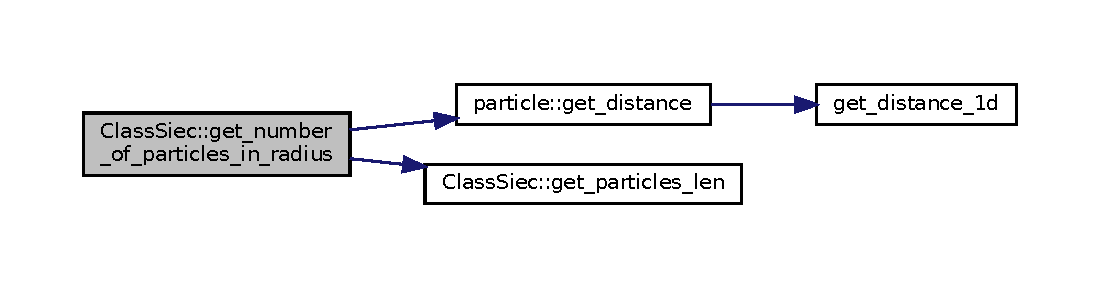
\includegraphics[width=350pt]{classClassSiec_ac5f8e08337a1ef96531495a6aee8bfb9_cgraph}
\end{center}
\end{figure}
\mbox{\Hypertarget{classClassSiec_a0c89392852117a823a1a603f4181b3a7}\label{classClassSiec_a0c89392852117a823a1a603f4181b3a7}} 
\index{Class\+Siec@{Class\+Siec}!get\+\_\+number\+\_\+of\+\_\+particles\+\_\+in\+\_\+radius@{get\+\_\+number\+\_\+of\+\_\+particles\+\_\+in\+\_\+radius}}
\index{get\+\_\+number\+\_\+of\+\_\+particles\+\_\+in\+\_\+radius@{get\+\_\+number\+\_\+of\+\_\+particles\+\_\+in\+\_\+radius}!Class\+Siec@{Class\+Siec}}
\subsubsection{\texorpdfstring{get\+\_\+number\+\_\+of\+\_\+particles\+\_\+in\+\_\+radius()}{get\_number\_of\_particles\_in\_radius()}\hspace{0.1cm}{\footnotesize\ttfamily [2/2]}}
{\footnotesize\ttfamily uint64\+\_\+t Class\+Siec\+::get\+\_\+number\+\_\+of\+\_\+particles\+\_\+in\+\_\+radius (\begin{DoxyParamCaption}\item[{double}]{r,  }\item[{double}]{dr }\end{DoxyParamCaption})}

Get number of particles in radius of each particles 
\begin{DoxyParams}{Parameters}
{\em r} & \\
\hline
{\em dr} & \\
\hline
\end{DoxyParams}
\begin{DoxyReturn}{Returns}

\end{DoxyReturn}


Definition at line 1262 of file Class\+Siec.\+cpp.



References box\+\_\+x, box\+\_\+y, get\+\_\+distance\+\_\+2d(), get\+\_\+particles\+\_\+len(), and particles.

Here is the call graph for this function\+:
\nopagebreak
\begin{figure}[H]
\begin{center}
\leavevmode
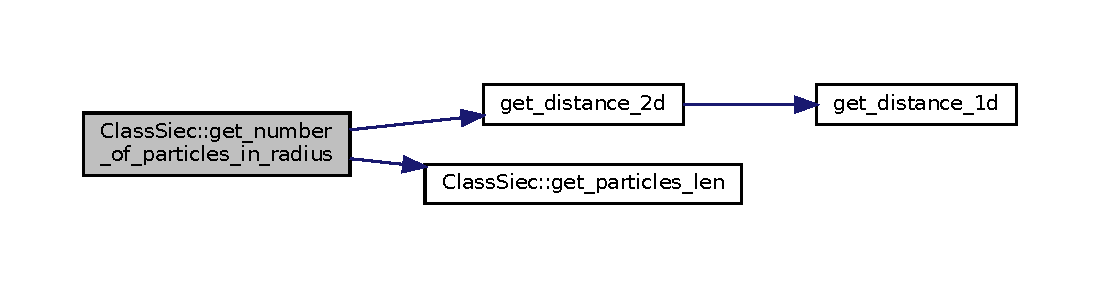
\includegraphics[width=350pt]{classClassSiec_a0c89392852117a823a1a603f4181b3a7_cgraph}
\end{center}
\end{figure}
\mbox{\Hypertarget{classClassSiec_a1b7f3db9473b2660b3a6c1dfeee45e22}\label{classClassSiec_a1b7f3db9473b2660b3a6c1dfeee45e22}} 
\index{Class\+Siec@{Class\+Siec}!get\+\_\+packing\+\_\+ratio@{get\+\_\+packing\+\_\+ratio}}
\index{get\+\_\+packing\+\_\+ratio@{get\+\_\+packing\+\_\+ratio}!Class\+Siec@{Class\+Siec}}
\subsubsection{\texorpdfstring{get\+\_\+packing\+\_\+ratio()}{get\_packing\_ratio()}}
{\footnotesize\ttfamily float Class\+Siec\+::get\+\_\+packing\+\_\+ratio (\begin{DoxyParamCaption}\item[{void}]{ }\end{DoxyParamCaption})}

Get the packing ratio of the particles in the box \begin{DoxyReturn}{Returns}

\end{DoxyReturn}


Definition at line 1197 of file Class\+Siec.\+cpp.



References box\+\_\+x, box\+\_\+y, get\+\_\+particles\+\_\+len(), and particles.



Referenced by get\+\_\+radial\+\_\+distribution\+\_\+function\+\_\+theoretical(), get\+\_\+state\+\_\+space\+\_\+\+Boublik(), get\+\_\+state\+\_\+space\+\_\+\+Handerson(), get\+\_\+state\+\_\+space\+\_\+\+Solan(), get\+\_\+static\+\_\+parameters\+\_\+info(), and get\+\_\+static\+\_\+parameters\+\_\+raw().

Here is the call graph for this function\+:
\nopagebreak
\begin{figure}[H]
\begin{center}
\leavevmode
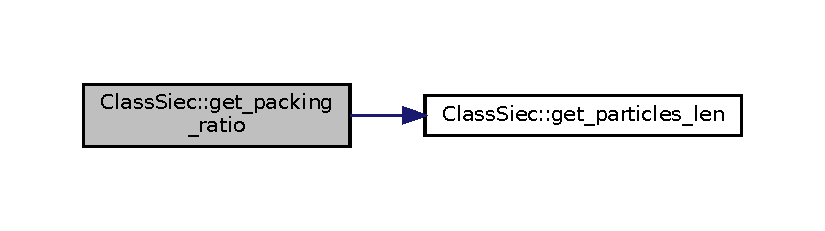
\includegraphics[width=350pt]{classClassSiec_a1b7f3db9473b2660b3a6c1dfeee45e22_cgraph}
\end{center}
\end{figure}
\mbox{\Hypertarget{classClassSiec_aa4c36868471f5747008cea881f1038c1}\label{classClassSiec_aa4c36868471f5747008cea881f1038c1}} 
\index{Class\+Siec@{Class\+Siec}!get\+\_\+particle@{get\+\_\+particle}}
\index{get\+\_\+particle@{get\+\_\+particle}!Class\+Siec@{Class\+Siec}}
\subsubsection{\texorpdfstring{get\+\_\+particle()}{get\_particle()}}
{\footnotesize\ttfamily int Class\+Siec\+::get\+\_\+particle (\begin{DoxyParamCaption}\item[{uint64\+\_\+t}]{nr,  }\item[{\mbox{\hyperlink{structparticle}{particle}} $\ast$}]{here }\end{DoxyParamCaption})}

Get address of particle with number to destination \begin{DoxyRefDesc}{Todo}
\item[\mbox{\hyperlink{todo__todo000004}{Todo}}]Probably useless \end{DoxyRefDesc}

\begin{DoxyParams}{Parameters}
{\em nr} & \\
\hline
{\em here} & \\
\hline
\end{DoxyParams}
\begin{DoxyReturn}{Returns}

\end{DoxyReturn}


Definition at line 830 of file Class\+Siec.\+cpp.



References E\+R\+R\+OR, OK, and particles.

\mbox{\Hypertarget{classClassSiec_a5fa315d36ce3648e5e5c2bf66b744e18}\label{classClassSiec_a5fa315d36ce3648e5e5c2bf66b744e18}} 
\index{Class\+Siec@{Class\+Siec}!get\+\_\+particles\+\_\+len@{get\+\_\+particles\+\_\+len}}
\index{get\+\_\+particles\+\_\+len@{get\+\_\+particles\+\_\+len}!Class\+Siec@{Class\+Siec}}
\subsubsection{\texorpdfstring{get\+\_\+particles\+\_\+len()}{get\_particles\_len()}}
{\footnotesize\ttfamily uint64\+\_\+t Class\+Siec\+::get\+\_\+particles\+\_\+len (\begin{DoxyParamCaption}\item[{void}]{ }\end{DoxyParamCaption})}

\begin{DoxyReturn}{Returns}
numbers of particles 
\end{DoxyReturn}


Definition at line 415 of file Class\+Siec.\+cpp.



References particles.



Referenced by draw\+\_\+all(), fix\+\_\+position(), get\+\_\+density(), get\+\_\+density\+\_\+real(), get\+\_\+kinetic\+\_\+energy(), get\+\_\+max\+\_\+radius(), get\+\_\+min\+\_\+radius(), get\+\_\+next\+\_\+collision\+\_\+particle\+\_\+number(), get\+\_\+next\+\_\+collision\+\_\+particles(), get\+\_\+number\+\_\+of\+\_\+particles\+\_\+in\+\_\+radius(), get\+\_\+packing\+\_\+ratio(), get\+\_\+\+R\+D\+F\+\_\+r(), get\+\_\+static\+\_\+parameters\+\_\+info(), get\+\_\+temperature(), get\+\_\+\+Velocity\+\_\+\+Autocorrelation\+\_\+\+Function(), save\+\_\+\+R\+D\+F(), save\+\_\+\+R\+D\+F\+\_\+to\+\_\+array(), set\+\_\+mass\+\_\+all(), set\+\_\+mass\+\_\+to\+\_\+area(), set\+\_\+mass\+\_\+to\+\_\+radius(), set\+\_\+momentum\+\_\+to\+\_\+zero(), set\+\_\+particles\+\_\+zero\+\_\+time(), set\+\_\+random\+\_\+size(), set\+\_\+random\+\_\+velocity(), step\+\_\+all(), and thread\+\_\+\+R\+D\+F().

\mbox{\Hypertarget{classClassSiec_a1a3c05e29d9fb646f1733704db81933d}\label{classClassSiec_a1a3c05e29d9fb646f1733704db81933d}} 
\index{Class\+Siec@{Class\+Siec}!get\+\_\+radial\+\_\+distribution\+\_\+function@{get\+\_\+radial\+\_\+distribution\+\_\+function}}
\index{get\+\_\+radial\+\_\+distribution\+\_\+function@{get\+\_\+radial\+\_\+distribution\+\_\+function}!Class\+Siec@{Class\+Siec}}
\subsubsection{\texorpdfstring{get\+\_\+radial\+\_\+distribution\+\_\+function()}{get\_radial\_distribution\_function()}\hspace{0.1cm}{\footnotesize\ttfamily [1/2]}}
{\footnotesize\ttfamily float Class\+Siec\+::get\+\_\+radial\+\_\+distribution\+\_\+function (\begin{DoxyParamCaption}\item[{double}]{r,  }\item[{double}]{dr,  }\item[{\mbox{\hyperlink{structparticle}{particle}} $\ast$}]{for\+\_\+particle,  }\item[{uint64\+\_\+t}]{prec = {\ttfamily 100} }\end{DoxyParamCaption})}

Get Radial distribution Function for particle 
\begin{DoxyParams}{Parameters}
{\em r} & \\
\hline
{\em dr} & \\
\hline
{\em for\+\_\+particle} & \\
\hline
{\em prec} & -\/$>$ divide dr into \textquotesingle{}prec\textquotesingle{} parts zrobic histogramy dla wszystkich kulek i liczyc g(r) od (r/d) lub (r/sigma) \\
\hline
\end{DoxyParams}
\begin{DoxyReturn}{Returns}

\end{DoxyReturn}


Definition at line 1296 of file Class\+Siec.\+cpp.



References current\+\_\+\+R\+DF, get\+\_\+density(), and get\+\_\+number\+\_\+of\+\_\+particles\+\_\+in\+\_\+radius().



Referenced by step\+\_\+all().

Here is the call graph for this function\+:
\nopagebreak
\begin{figure}[H]
\begin{center}
\leavevmode
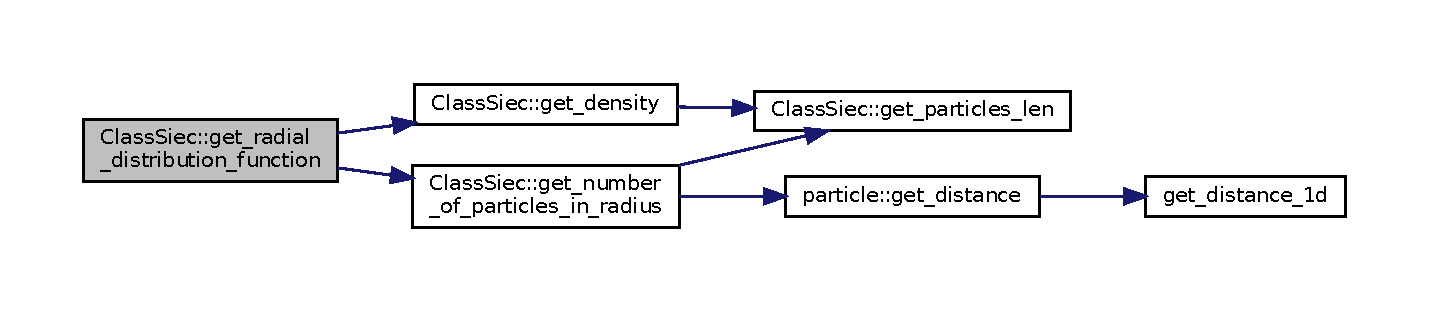
\includegraphics[width=350pt]{classClassSiec_a1a3c05e29d9fb646f1733704db81933d_cgraph}
\end{center}
\end{figure}
\mbox{\Hypertarget{classClassSiec_a95685407da49bfa4d1a54fd248e8aee3}\label{classClassSiec_a95685407da49bfa4d1a54fd248e8aee3}} 
\index{Class\+Siec@{Class\+Siec}!get\+\_\+radial\+\_\+distribution\+\_\+function@{get\+\_\+radial\+\_\+distribution\+\_\+function}}
\index{get\+\_\+radial\+\_\+distribution\+\_\+function@{get\+\_\+radial\+\_\+distribution\+\_\+function}!Class\+Siec@{Class\+Siec}}
\subsubsection{\texorpdfstring{get\+\_\+radial\+\_\+distribution\+\_\+function()}{get\_radial\_distribution\_function()}\hspace{0.1cm}{\footnotesize\ttfamily [2/2]}}
{\footnotesize\ttfamily float Class\+Siec\+::get\+\_\+radial\+\_\+distribution\+\_\+function (\begin{DoxyParamCaption}\item[{double}]{r,  }\item[{double}]{dr }\end{DoxyParamCaption})}

Get Radial distribution Function \begin{DoxyRefDesc}{Bug}
\item[\mbox{\hyperlink{bug__bug000003}{Bug}}]probably bad function \end{DoxyRefDesc}

\begin{DoxyParams}{Parameters}
{\em r} & \\
\hline
{\em dr} & \\
\hline
\end{DoxyParams}
\begin{DoxyReturn}{Returns}

\end{DoxyReturn}


Definition at line 1328 of file Class\+Siec.\+cpp.



References get\+\_\+density(), and get\+\_\+number\+\_\+of\+\_\+particles\+\_\+in\+\_\+radius().

Here is the call graph for this function\+:
\nopagebreak
\begin{figure}[H]
\begin{center}
\leavevmode
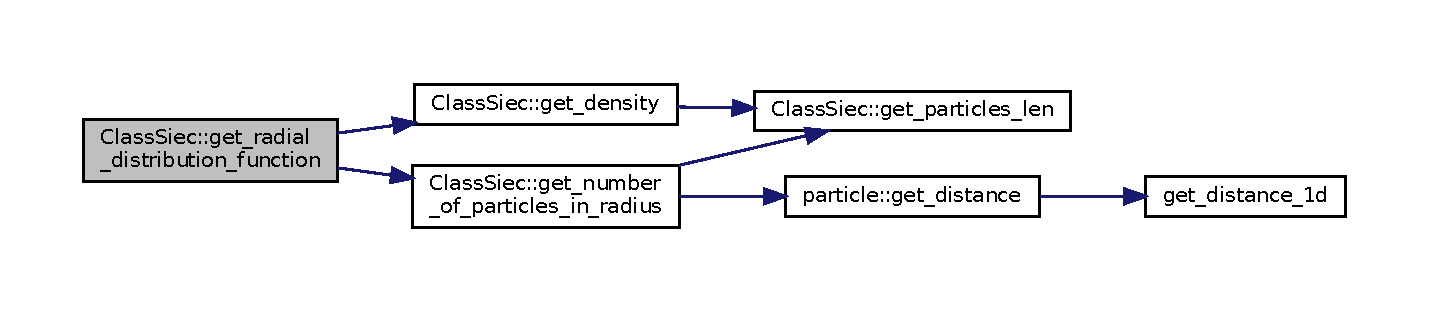
\includegraphics[width=350pt]{classClassSiec_a95685407da49bfa4d1a54fd248e8aee3_cgraph}
\end{center}
\end{figure}
\mbox{\Hypertarget{classClassSiec_a87284d96c487a462bf8a42d81fc4bb8c}\label{classClassSiec_a87284d96c487a462bf8a42d81fc4bb8c}} 
\index{Class\+Siec@{Class\+Siec}!get\+\_\+radial\+\_\+distribution\+\_\+function\+\_\+theoretical@{get\+\_\+radial\+\_\+distribution\+\_\+function\+\_\+theoretical}}
\index{get\+\_\+radial\+\_\+distribution\+\_\+function\+\_\+theoretical@{get\+\_\+radial\+\_\+distribution\+\_\+function\+\_\+theoretical}!Class\+Siec@{Class\+Siec}}
\subsubsection{\texorpdfstring{get\+\_\+radial\+\_\+distribution\+\_\+function\+\_\+theoretical()}{get\_radial\_distribution\_function\_theoretical()}}
{\footnotesize\ttfamily float Class\+Siec\+::get\+\_\+radial\+\_\+distribution\+\_\+function\+\_\+theoretical (\begin{DoxyParamCaption}\item[{void}]{ }\end{DoxyParamCaption})}

Get Radial distribution Function -\/ theoretical \begin{DoxyRefDesc}{Todo}
\item[\mbox{\hyperlink{todo__todo000005}{Todo}}]Check this \end{DoxyRefDesc}
\begin{DoxyReturn}{Returns}

\end{DoxyReturn}


Definition at line 1339 of file Class\+Siec.\+cpp.



References get\+\_\+packing\+\_\+ratio().



Referenced by get\+\_\+static\+\_\+parameters\+\_\+info().

Here is the call graph for this function\+:
\nopagebreak
\begin{figure}[H]
\begin{center}
\leavevmode
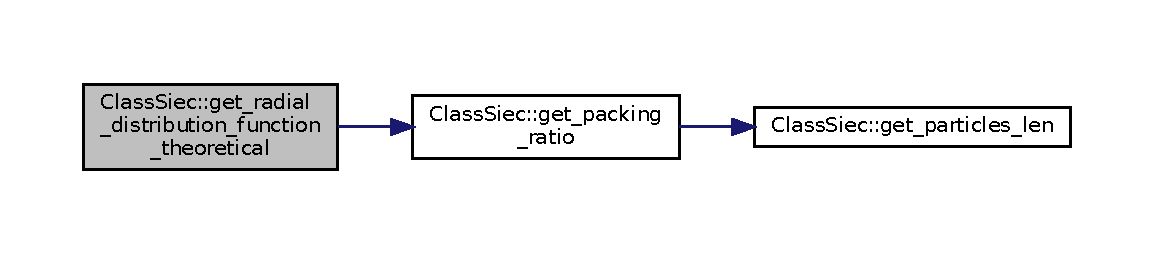
\includegraphics[width=350pt]{classClassSiec_a87284d96c487a462bf8a42d81fc4bb8c_cgraph}
\end{center}
\end{figure}
\mbox{\Hypertarget{classClassSiec_a609cc786246741388e18ed50c0165388}\label{classClassSiec_a609cc786246741388e18ed50c0165388}} 
\index{Class\+Siec@{Class\+Siec}!get\+\_\+\+R\+D\+F\+\_\+r@{get\+\_\+\+R\+D\+F\+\_\+r}}
\index{get\+\_\+\+R\+D\+F\+\_\+r@{get\+\_\+\+R\+D\+F\+\_\+r}!Class\+Siec@{Class\+Siec}}
\subsubsection{\texorpdfstring{get\+\_\+\+R\+D\+F\+\_\+r()}{get\_RDF\_r()}\hspace{0.1cm}{\footnotesize\ttfamily [1/2]}}
{\footnotesize\ttfamily std\+::string Class\+Siec\+::get\+\_\+\+R\+D\+F\+\_\+r (\begin{DoxyParamCaption}\item[{double}]{r,  }\item[{double}]{dr,  }\item[{uint64\+\_\+t}]{prec = {\ttfamily 100},  }\item[{std\+::string}]{sep = {\ttfamily \char`\"{}~\char`\"{}} }\end{DoxyParamCaption})}

Get R\+DF 
\begin{DoxyParams}{Parameters}
{\em r} & \\
\hline
{\em dr} & \\
\hline
{\em prec} & \\
\hline
{\em sep} & \\
\hline
\end{DoxyParams}
\begin{DoxyReturn}{Returns}

\end{DoxyReturn}


Definition at line 1625 of file Class\+Siec.\+cpp.



References get\+\_\+density(), get\+\_\+number\+\_\+of\+\_\+particles\+\_\+in\+\_\+radius(), get\+\_\+particles\+\_\+len(), and particles.



Referenced by get\+\_\+\+R\+D\+F\+\_\+r().

Here is the call graph for this function\+:
\nopagebreak
\begin{figure}[H]
\begin{center}
\leavevmode
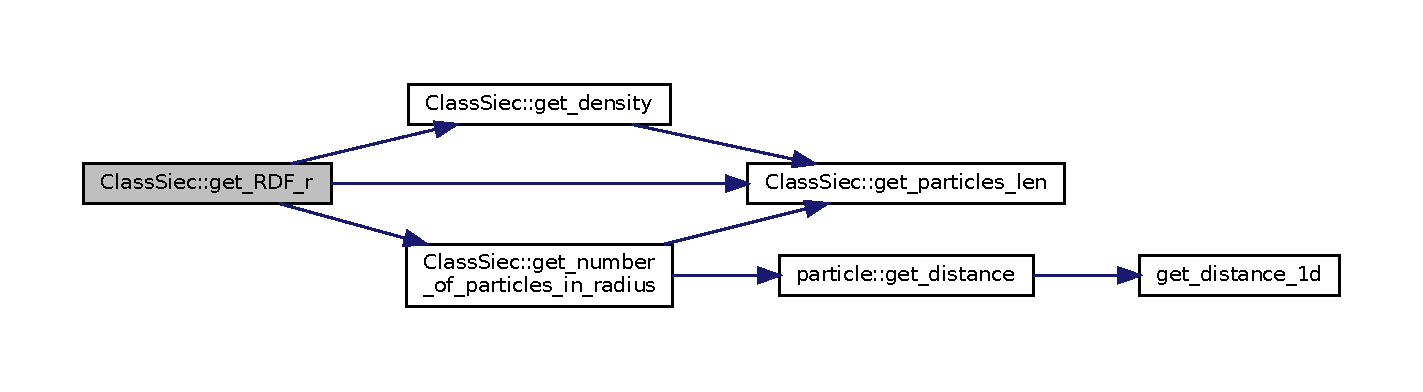
\includegraphics[width=350pt]{classClassSiec_a609cc786246741388e18ed50c0165388_cgraph}
\end{center}
\end{figure}
\mbox{\Hypertarget{classClassSiec_aad7c55f1dfa1b5bca25fc39e0b509304}\label{classClassSiec_aad7c55f1dfa1b5bca25fc39e0b509304}} 
\index{Class\+Siec@{Class\+Siec}!get\+\_\+\+R\+D\+F\+\_\+r@{get\+\_\+\+R\+D\+F\+\_\+r}}
\index{get\+\_\+\+R\+D\+F\+\_\+r@{get\+\_\+\+R\+D\+F\+\_\+r}!Class\+Siec@{Class\+Siec}}
\subsubsection{\texorpdfstring{get\+\_\+\+R\+D\+F\+\_\+r()}{get\_RDF\_r()}\hspace{0.1cm}{\footnotesize\ttfamily [2/2]}}
{\footnotesize\ttfamily std\+::string Class\+Siec\+::get\+\_\+\+R\+D\+F\+\_\+r (\begin{DoxyParamCaption}\item[{uint64\+\_\+t}]{prec = {\ttfamily 100},  }\item[{std\+::string}]{sep = {\ttfamily \char`\"{}~\char`\"{}} }\end{DoxyParamCaption})}

Get default R\+DF 
\begin{DoxyParams}{Parameters}
{\em prec} & \\
\hline
{\em sep} & \\
\hline
\end{DoxyParams}
\begin{DoxyReturn}{Returns}

\end{DoxyReturn}


Definition at line 1666 of file Class\+Siec.\+cpp.



References box\+\_\+x, box\+\_\+y, and get\+\_\+\+R\+D\+F\+\_\+r().

Here is the call graph for this function\+:
\nopagebreak
\begin{figure}[H]
\begin{center}
\leavevmode
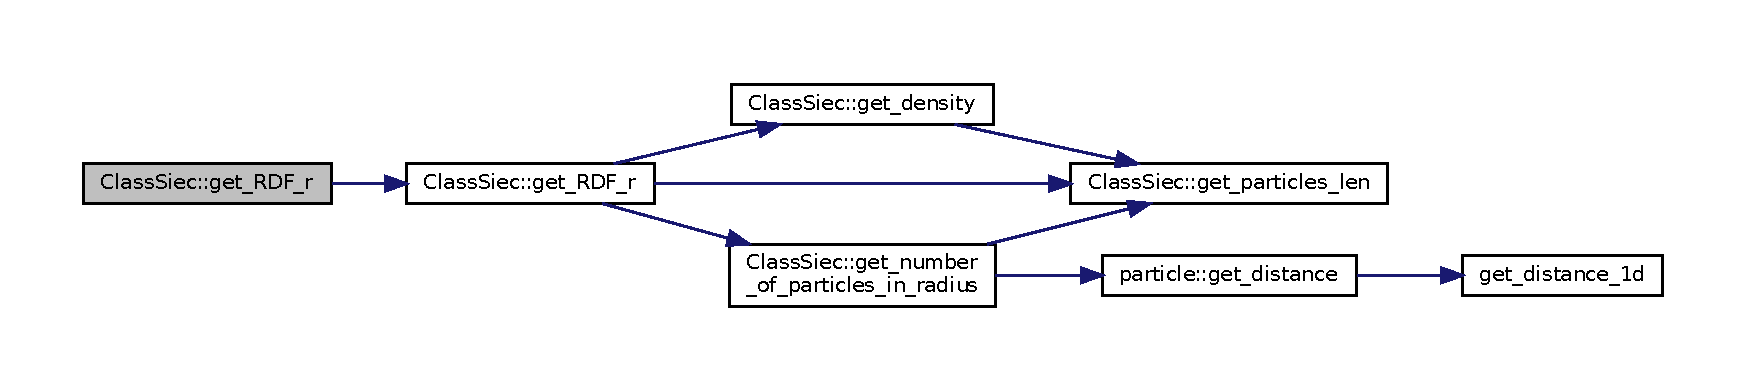
\includegraphics[width=350pt]{classClassSiec_aad7c55f1dfa1b5bca25fc39e0b509304_cgraph}
\end{center}
\end{figure}
\mbox{\Hypertarget{classClassSiec_a8fb2e1fa04229aaa6027fed8dd996aea}\label{classClassSiec_a8fb2e1fa04229aaa6027fed8dd996aea}} 
\index{Class\+Siec@{Class\+Siec}!get\+\_\+state\+\_\+space\+\_\+\+Boublik@{get\+\_\+state\+\_\+space\+\_\+\+Boublik}}
\index{get\+\_\+state\+\_\+space\+\_\+\+Boublik@{get\+\_\+state\+\_\+space\+\_\+\+Boublik}!Class\+Siec@{Class\+Siec}}
\subsubsection{\texorpdfstring{get\+\_\+state\+\_\+space\+\_\+\+Boublik()}{get\_state\_space\_Boublik()}}
{\footnotesize\ttfamily float Class\+Siec\+::get\+\_\+state\+\_\+space\+\_\+\+Boublik (\begin{DoxyParamCaption}\item[{void}]{ }\end{DoxyParamCaption})}

Get state space -\/ Boublik \begin{DoxyReturn}{Returns}

\end{DoxyReturn}


Definition at line 1349 of file Class\+Siec.\+cpp.



References get\+\_\+density(), get\+\_\+packing\+\_\+ratio(), get\+\_\+temperature(), and k\+Boltzmann.



Referenced by get\+\_\+static\+\_\+parameters\+\_\+info(), and get\+\_\+static\+\_\+parameters\+\_\+raw().

Here is the call graph for this function\+:
\nopagebreak
\begin{figure}[H]
\begin{center}
\leavevmode
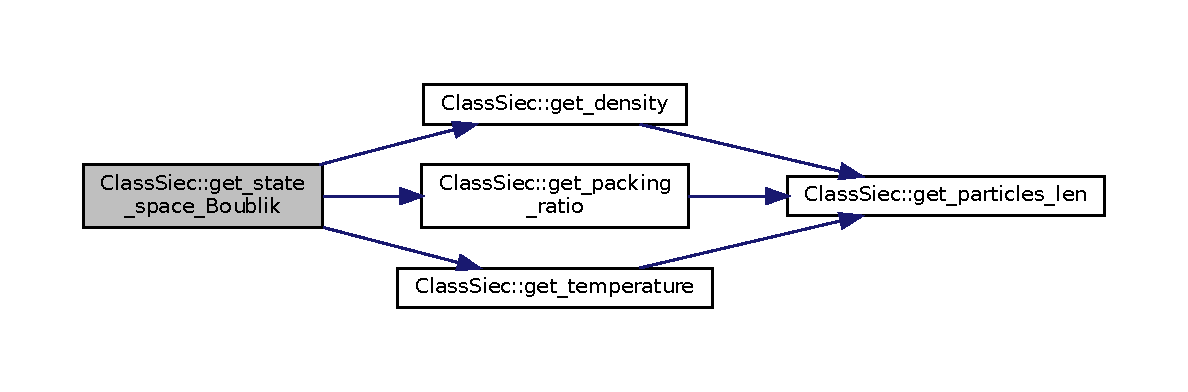
\includegraphics[width=350pt]{classClassSiec_a8fb2e1fa04229aaa6027fed8dd996aea_cgraph}
\end{center}
\end{figure}
\mbox{\Hypertarget{classClassSiec_a36144a1734674d3f0c6899c348da1a97}\label{classClassSiec_a36144a1734674d3f0c6899c348da1a97}} 
\index{Class\+Siec@{Class\+Siec}!get\+\_\+state\+\_\+space\+\_\+\+Handerson@{get\+\_\+state\+\_\+space\+\_\+\+Handerson}}
\index{get\+\_\+state\+\_\+space\+\_\+\+Handerson@{get\+\_\+state\+\_\+space\+\_\+\+Handerson}!Class\+Siec@{Class\+Siec}}
\subsubsection{\texorpdfstring{get\+\_\+state\+\_\+space\+\_\+\+Handerson()}{get\_state\_space\_Handerson()}}
{\footnotesize\ttfamily float Class\+Siec\+::get\+\_\+state\+\_\+space\+\_\+\+Handerson (\begin{DoxyParamCaption}\item[{void}]{ }\end{DoxyParamCaption})}

Get state space -\/ Handerson \begin{DoxyReturn}{Returns}

\end{DoxyReturn}


Definition at line 1363 of file Class\+Siec.\+cpp.



References get\+\_\+density(), get\+\_\+packing\+\_\+ratio(), get\+\_\+temperature(), and k\+Boltzmann.



Referenced by get\+\_\+static\+\_\+parameters\+\_\+info(), and get\+\_\+static\+\_\+parameters\+\_\+raw().

Here is the call graph for this function\+:
\nopagebreak
\begin{figure}[H]
\begin{center}
\leavevmode
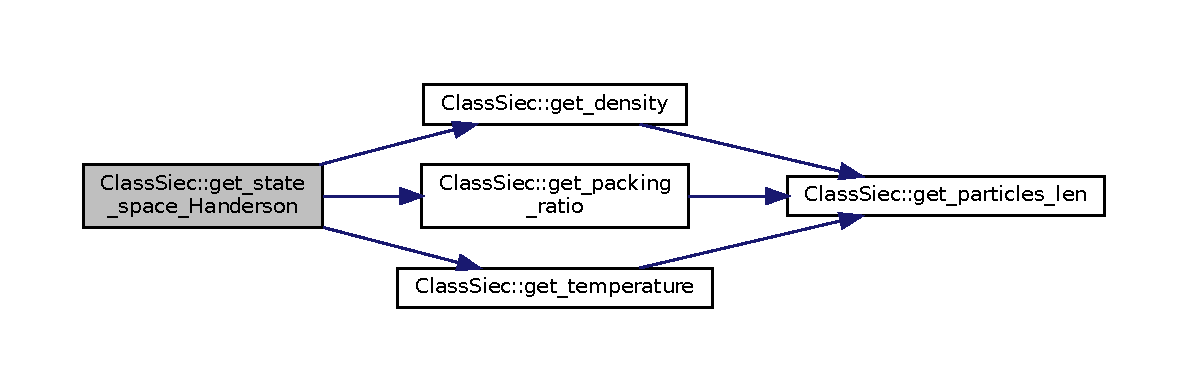
\includegraphics[width=350pt]{classClassSiec_a36144a1734674d3f0c6899c348da1a97_cgraph}
\end{center}
\end{figure}
\mbox{\Hypertarget{classClassSiec_a3a0171519c3557d8edec22edb5978c9c}\label{classClassSiec_a3a0171519c3557d8edec22edb5978c9c}} 
\index{Class\+Siec@{Class\+Siec}!get\+\_\+state\+\_\+space\+\_\+\+Solan@{get\+\_\+state\+\_\+space\+\_\+\+Solan}}
\index{get\+\_\+state\+\_\+space\+\_\+\+Solan@{get\+\_\+state\+\_\+space\+\_\+\+Solan}!Class\+Siec@{Class\+Siec}}
\subsubsection{\texorpdfstring{get\+\_\+state\+\_\+space\+\_\+\+Solan()}{get\_state\_space\_Solan()}}
{\footnotesize\ttfamily float Class\+Siec\+::get\+\_\+state\+\_\+space\+\_\+\+Solan (\begin{DoxyParamCaption}\item[{void}]{ }\end{DoxyParamCaption})}

Get state space -\/ Solan \begin{DoxyReturn}{Returns}

\end{DoxyReturn}


Definition at line 1374 of file Class\+Siec.\+cpp.



References get\+\_\+density(), get\+\_\+packing\+\_\+ratio(), get\+\_\+temperature(), and k\+Boltzmann.



Referenced by get\+\_\+static\+\_\+parameters\+\_\+info(), and get\+\_\+static\+\_\+parameters\+\_\+raw().

Here is the call graph for this function\+:
\nopagebreak
\begin{figure}[H]
\begin{center}
\leavevmode
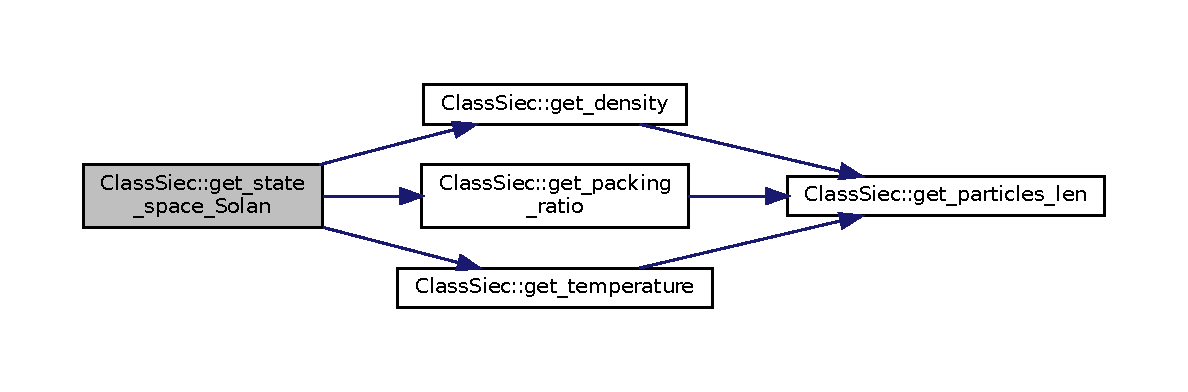
\includegraphics[width=350pt]{classClassSiec_a3a0171519c3557d8edec22edb5978c9c_cgraph}
\end{center}
\end{figure}
\mbox{\Hypertarget{classClassSiec_aaf3b24bc73d268f151acdff6351214e0}\label{classClassSiec_aaf3b24bc73d268f151acdff6351214e0}} 
\index{Class\+Siec@{Class\+Siec}!get\+\_\+static\+\_\+parameters\+\_\+info@{get\+\_\+static\+\_\+parameters\+\_\+info}}
\index{get\+\_\+static\+\_\+parameters\+\_\+info@{get\+\_\+static\+\_\+parameters\+\_\+info}!Class\+Siec@{Class\+Siec}}
\subsubsection{\texorpdfstring{get\+\_\+static\+\_\+parameters\+\_\+info()}{get\_static\_parameters\_info()}}
{\footnotesize\ttfamily std\+::string Class\+Siec\+::get\+\_\+static\+\_\+parameters\+\_\+info (\begin{DoxyParamCaption}\item[{std\+::string}]{sep = {\ttfamily \char`\"{}\textbackslash{}n\char`\"{}} }\end{DoxyParamCaption})}

Get static parameters full 
\begin{DoxyParams}{Parameters}
{\em sep} & \\
\hline
\end{DoxyParams}
\begin{DoxyReturn}{Returns}

\end{DoxyReturn}


Definition at line 1800 of file Class\+Siec.\+cpp.



References get\+\_\+density(), get\+\_\+density\+\_\+real(), get\+\_\+diffusitivity\+\_\+delta(), get\+\_\+diffusitivity\+\_\+delta\+\_\+ratio(), get\+\_\+diffusivity(), get\+\_\+packing\+\_\+ratio(), get\+\_\+particles\+\_\+len(), get\+\_\+radial\+\_\+distribution\+\_\+function\+\_\+theoretical(), get\+\_\+state\+\_\+space\+\_\+\+Boublik(), get\+\_\+state\+\_\+space\+\_\+\+Handerson(), get\+\_\+state\+\_\+space\+\_\+\+Solan(), get\+\_\+temperature(), and get\+\_\+\+Velocity\+\_\+\+Autocorrelation\+\_\+\+Function().



Referenced by main().

Here is the call graph for this function\+:
\nopagebreak
\begin{figure}[H]
\begin{center}
\leavevmode
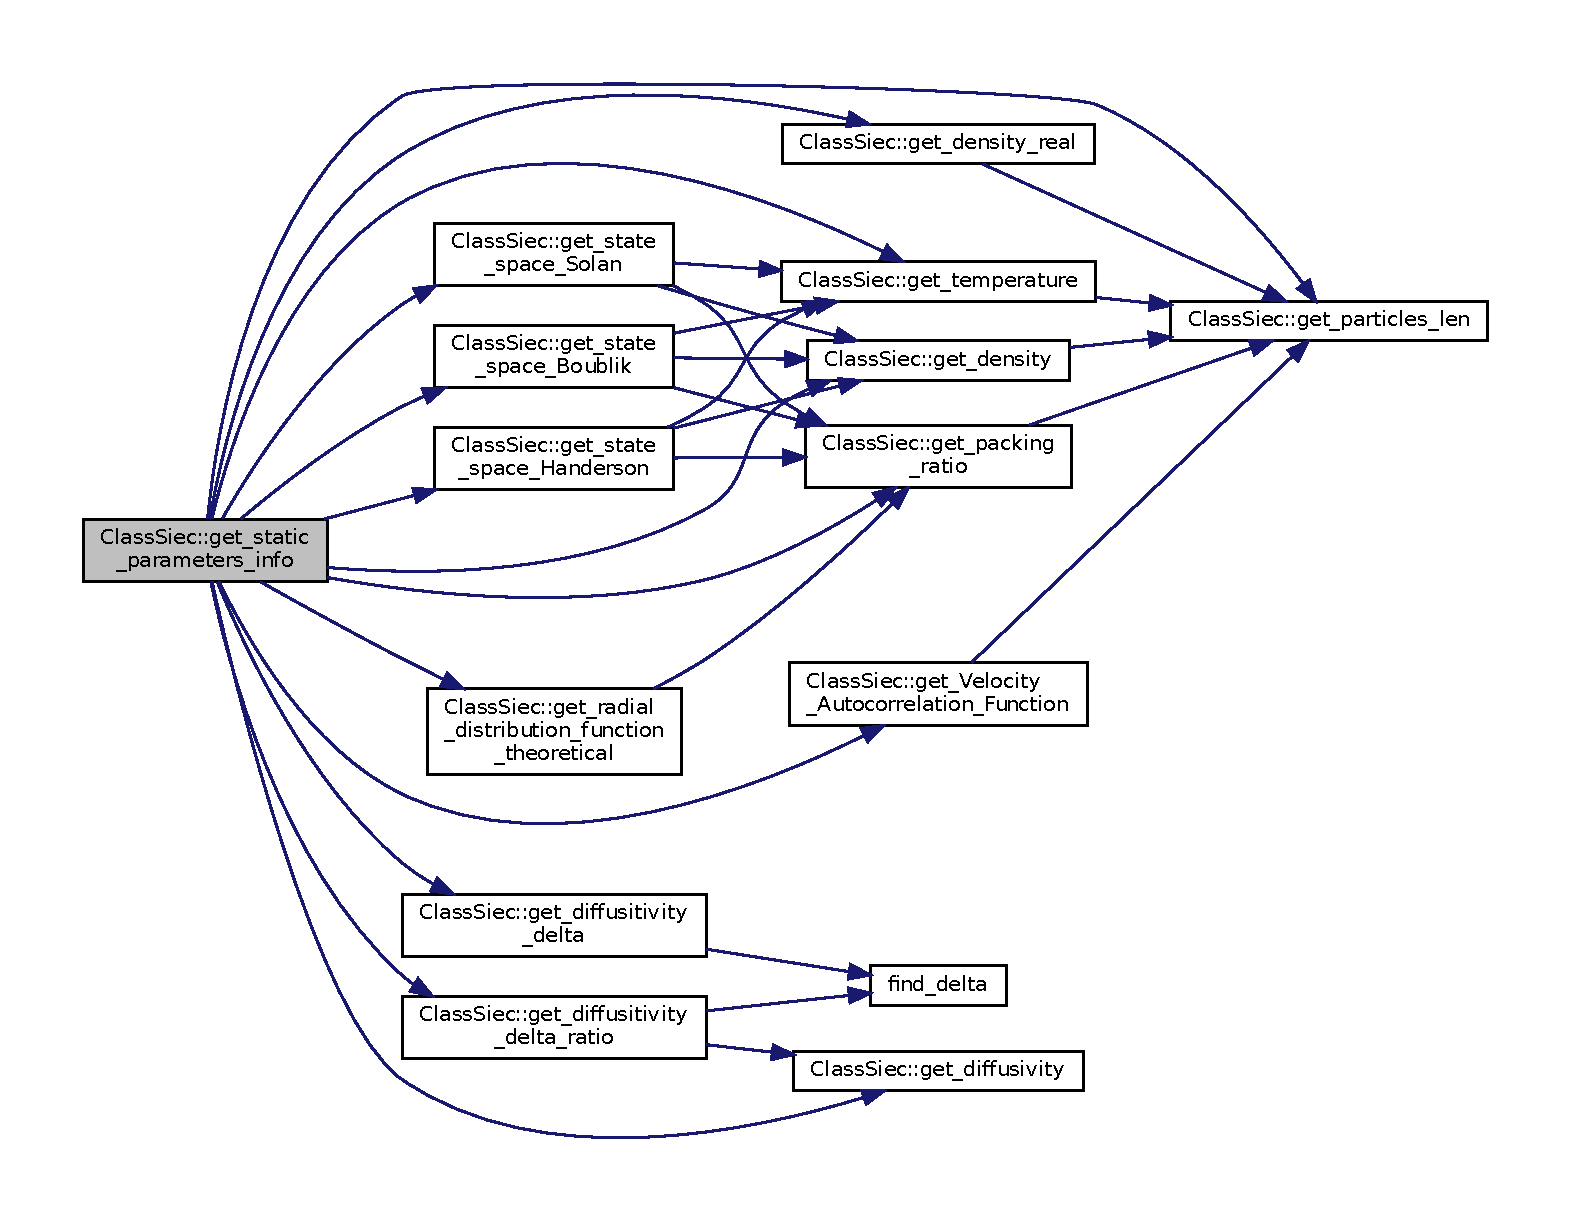
\includegraphics[width=350pt]{classClassSiec_aaf3b24bc73d268f151acdff6351214e0_cgraph}
\end{center}
\end{figure}
\mbox{\Hypertarget{classClassSiec_abed8d28e81524a99ab325569db15bb36}\label{classClassSiec_abed8d28e81524a99ab325569db15bb36}} 
\index{Class\+Siec@{Class\+Siec}!get\+\_\+static\+\_\+parameters\+\_\+raw@{get\+\_\+static\+\_\+parameters\+\_\+raw}}
\index{get\+\_\+static\+\_\+parameters\+\_\+raw@{get\+\_\+static\+\_\+parameters\+\_\+raw}!Class\+Siec@{Class\+Siec}}
\subsubsection{\texorpdfstring{get\+\_\+static\+\_\+parameters\+\_\+raw()}{get\_static\_parameters\_raw()}}
{\footnotesize\ttfamily std\+::string Class\+Siec\+::get\+\_\+static\+\_\+parameters\+\_\+raw (\begin{DoxyParamCaption}\item[{std\+::string}]{sep = {\ttfamily \char`\"{}\textbackslash{}t\char`\"{}} }\end{DoxyParamCaption})}

Get static parameters raw data only 
\begin{DoxyParams}{Parameters}
{\em sep} & \\
\hline
\end{DoxyParams}
\begin{DoxyReturn}{Returns}

\end{DoxyReturn}


Definition at line 1838 of file Class\+Siec.\+cpp.



References get\+\_\+density(), get\+\_\+density\+\_\+real(), get\+\_\+diffusitivity\+\_\+delta(), get\+\_\+diffusitivity\+\_\+delta\+\_\+ratio(), get\+\_\+diffusivity(), get\+\_\+packing\+\_\+ratio(), get\+\_\+state\+\_\+space\+\_\+\+Boublik(), get\+\_\+state\+\_\+space\+\_\+\+Handerson(), get\+\_\+state\+\_\+space\+\_\+\+Solan(), get\+\_\+temperature(), and get\+\_\+\+Velocity\+\_\+\+Autocorrelation\+\_\+\+Function().

Here is the call graph for this function\+:
\nopagebreak
\begin{figure}[H]
\begin{center}
\leavevmode
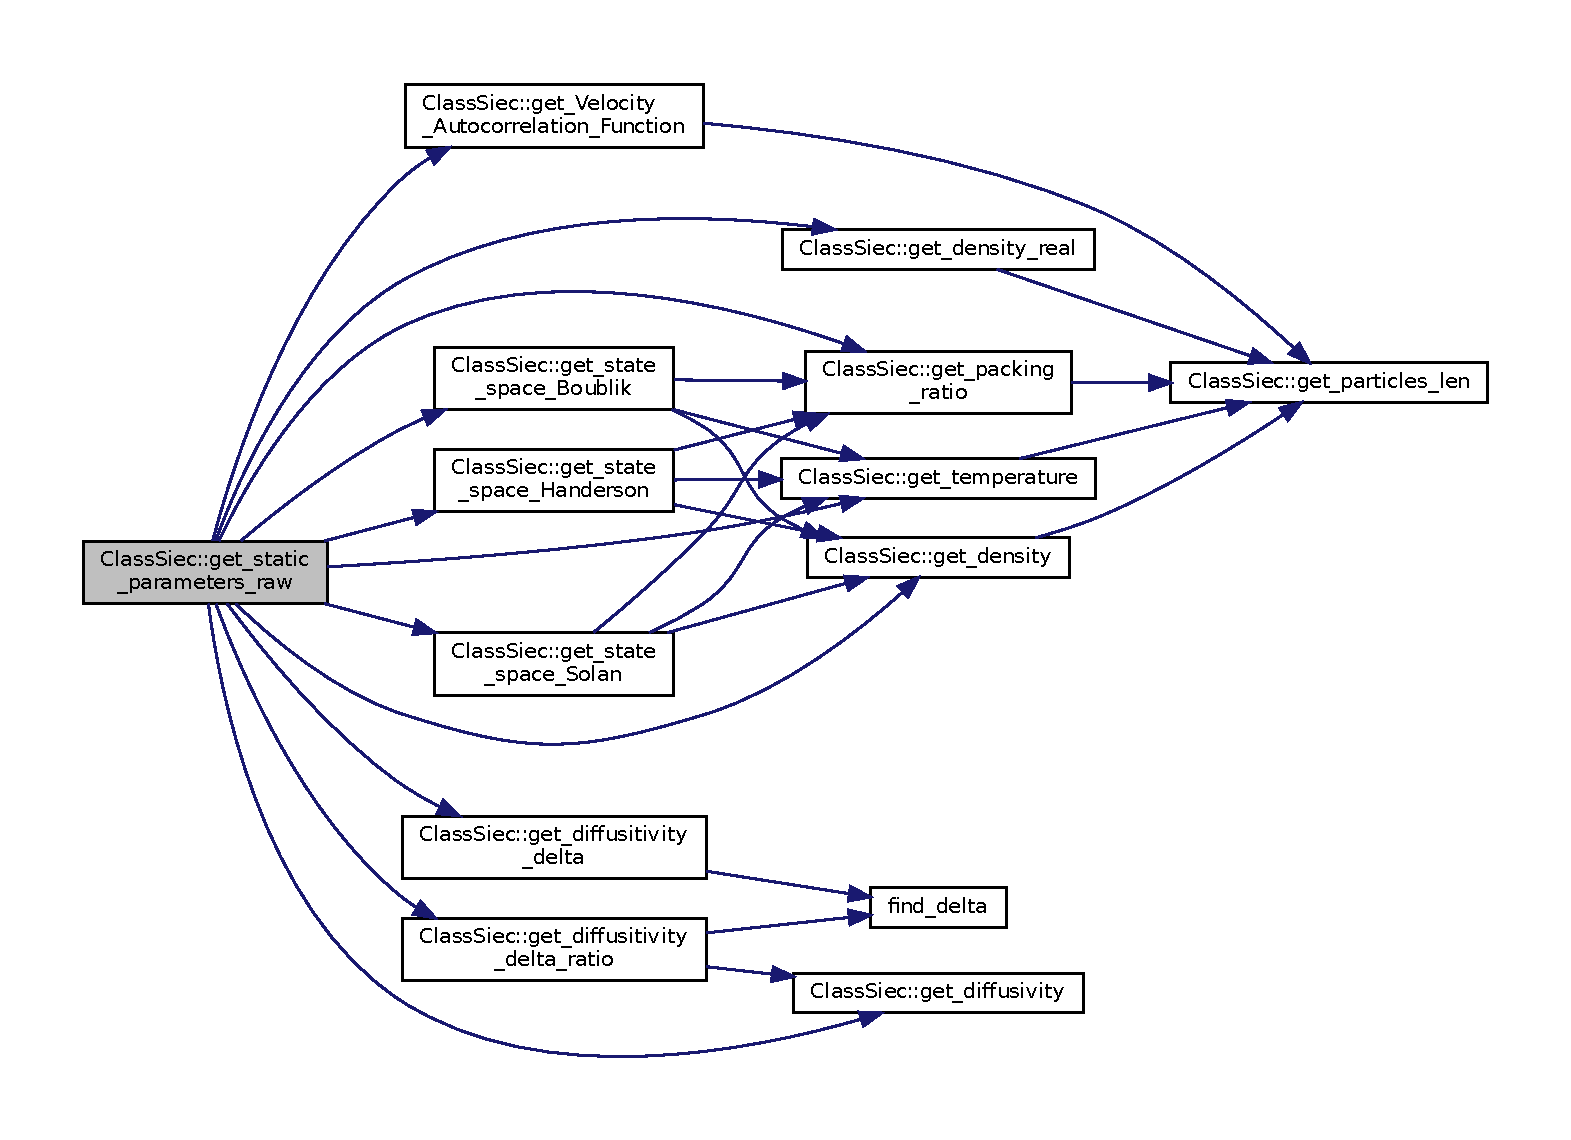
\includegraphics[width=350pt]{classClassSiec_abed8d28e81524a99ab325569db15bb36_cgraph}
\end{center}
\end{figure}
\mbox{\Hypertarget{classClassSiec_a1fcb70fc39cb91fe5b5382c7911de316}\label{classClassSiec_a1fcb70fc39cb91fe5b5382c7911de316}} 
\index{Class\+Siec@{Class\+Siec}!get\+\_\+static\+\_\+parameters\+\_\+title@{get\+\_\+static\+\_\+parameters\+\_\+title}}
\index{get\+\_\+static\+\_\+parameters\+\_\+title@{get\+\_\+static\+\_\+parameters\+\_\+title}!Class\+Siec@{Class\+Siec}}
\subsubsection{\texorpdfstring{get\+\_\+static\+\_\+parameters\+\_\+title()}{get\_static\_parameters\_title()}}
{\footnotesize\ttfamily std\+::string Class\+Siec\+::get\+\_\+static\+\_\+parameters\+\_\+title (\begin{DoxyParamCaption}\item[{std\+::string}]{sep = {\ttfamily \char`\"{}\textbackslash{}t\char`\"{}} }\end{DoxyParamCaption})}

Get static parameters only title 
\begin{DoxyParams}{Parameters}
{\em sep} & \\
\hline
\end{DoxyParams}
\begin{DoxyReturn}{Returns}

\end{DoxyReturn}


Definition at line 1769 of file Class\+Siec.\+cpp.

\mbox{\Hypertarget{classClassSiec_ae0e08ad933601148dcd2edc998c17a61}\label{classClassSiec_ae0e08ad933601148dcd2edc998c17a61}} 
\index{Class\+Siec@{Class\+Siec}!get\+\_\+temperature@{get\+\_\+temperature}}
\index{get\+\_\+temperature@{get\+\_\+temperature}!Class\+Siec@{Class\+Siec}}
\subsubsection{\texorpdfstring{get\+\_\+temperature()}{get\_temperature()}}
{\footnotesize\ttfamily float Class\+Siec\+::get\+\_\+temperature (\begin{DoxyParamCaption}\item[{void}]{ }\end{DoxyParamCaption})}

Get temperature \begin{DoxyReturn}{Returns}

\end{DoxyReturn}


Definition at line 1144 of file Class\+Siec.\+cpp.



References get\+\_\+particles\+\_\+len(), k\+Boltzmann, and particles.



Referenced by get\+\_\+state\+\_\+space\+\_\+\+Boublik(), get\+\_\+state\+\_\+space\+\_\+\+Handerson(), get\+\_\+state\+\_\+space\+\_\+\+Solan(), get\+\_\+static\+\_\+parameters\+\_\+info(), get\+\_\+static\+\_\+parameters\+\_\+raw(), and set\+\_\+momentum\+\_\+to\+\_\+zero().

Here is the call graph for this function\+:
\nopagebreak
\begin{figure}[H]
\begin{center}
\leavevmode
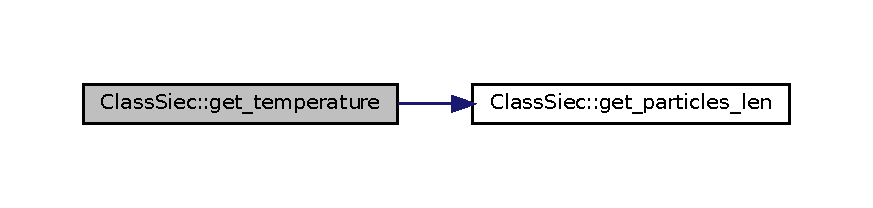
\includegraphics[width=350pt]{classClassSiec_ae0e08ad933601148dcd2edc998c17a61_cgraph}
\end{center}
\end{figure}
\mbox{\Hypertarget{classClassSiec_a27ab9475c3e1da5cba2c8dce28e12444}\label{classClassSiec_a27ab9475c3e1da5cba2c8dce28e12444}} 
\index{Class\+Siec@{Class\+Siec}!get\+\_\+time@{get\+\_\+time}}
\index{get\+\_\+time@{get\+\_\+time}!Class\+Siec@{Class\+Siec}}
\subsubsection{\texorpdfstring{get\+\_\+time()}{get\_time()}}
{\footnotesize\ttfamily float Class\+Siec\+::get\+\_\+time (\begin{DoxyParamCaption}\item[{void}]{ }\end{DoxyParamCaption})}



Definition at line 1135 of file Class\+Siec.\+cpp.



Referenced by thread\+\_\+siec().

\mbox{\Hypertarget{classClassSiec_acffa9f63d7236490d4e214a59e443140}\label{classClassSiec_acffa9f63d7236490d4e214a59e443140}} 
\index{Class\+Siec@{Class\+Siec}!get\+\_\+\+Velocity\+\_\+\+Autocorrelation\+\_\+\+Function@{get\+\_\+\+Velocity\+\_\+\+Autocorrelation\+\_\+\+Function}}
\index{get\+\_\+\+Velocity\+\_\+\+Autocorrelation\+\_\+\+Function@{get\+\_\+\+Velocity\+\_\+\+Autocorrelation\+\_\+\+Function}!Class\+Siec@{Class\+Siec}}
\subsubsection{\texorpdfstring{get\+\_\+\+Velocity\+\_\+\+Autocorrelation\+\_\+\+Function()}{get\_Velocity\_Autocorrelation\_Function()}}
{\footnotesize\ttfamily float Class\+Siec\+::get\+\_\+\+Velocity\+\_\+\+Autocorrelation\+\_\+\+Function (\begin{DoxyParamCaption}\item[{void}]{ }\end{DoxyParamCaption})}

Get Velocity Autocorrelation Function iloczyn skalarny vx(0)$\ast$vx(t) \begin{DoxyReturn}{Returns}

\end{DoxyReturn}


Definition at line 1388 of file Class\+Siec.\+cpp.



References get\+\_\+particles\+\_\+len(), particles, and particles\+\_\+zero\+\_\+time.



Referenced by get\+\_\+box\+\_\+info(), get\+\_\+box\+\_\+info\+\_\+raw(), get\+\_\+static\+\_\+parameters\+\_\+info(), get\+\_\+static\+\_\+parameters\+\_\+raw(), get\+\_\+\+Velocity\+\_\+\+Autocorrelation\+\_\+\+Function\+\_\+delta\+\_\+ratio(), step\+\_\+all(), and thread\+\_\+siec().

Here is the call graph for this function\+:
\nopagebreak
\begin{figure}[H]
\begin{center}
\leavevmode
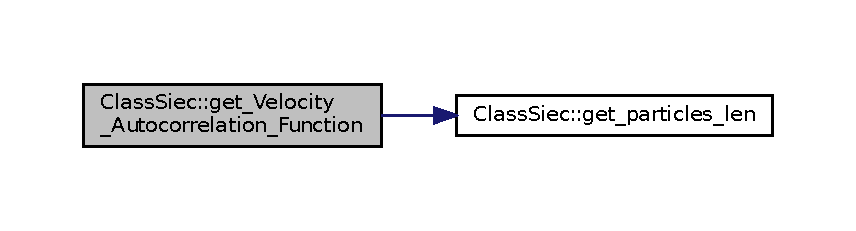
\includegraphics[width=350pt]{classClassSiec_acffa9f63d7236490d4e214a59e443140_cgraph}
\end{center}
\end{figure}
\mbox{\Hypertarget{classClassSiec_a21be4d09c7aa47a5d3f216509ad5feef}\label{classClassSiec_a21be4d09c7aa47a5d3f216509ad5feef}} 
\index{Class\+Siec@{Class\+Siec}!get\+\_\+\+Velocity\+\_\+\+Autocorrelation\+\_\+\+Function\+\_\+delta@{get\+\_\+\+Velocity\+\_\+\+Autocorrelation\+\_\+\+Function\+\_\+delta}}
\index{get\+\_\+\+Velocity\+\_\+\+Autocorrelation\+\_\+\+Function\+\_\+delta@{get\+\_\+\+Velocity\+\_\+\+Autocorrelation\+\_\+\+Function\+\_\+delta}!Class\+Siec@{Class\+Siec}}
\subsubsection{\texorpdfstring{get\+\_\+\+Velocity\+\_\+\+Autocorrelation\+\_\+\+Function\+\_\+delta()}{get\_Velocity\_Autocorrelation\_Function\_delta()}}
{\footnotesize\ttfamily double Class\+Siec\+::get\+\_\+\+Velocity\+\_\+\+Autocorrelation\+\_\+\+Function\+\_\+delta (\begin{DoxyParamCaption}\item[{void}]{ }\end{DoxyParamCaption})}



Definition at line 1431 of file Class\+Siec.\+cpp.



References find\+\_\+delta().



Referenced by get\+\_\+box\+\_\+info(), get\+\_\+box\+\_\+info\+\_\+raw(), and thread\+\_\+siec().

Here is the call graph for this function\+:
\nopagebreak
\begin{figure}[H]
\begin{center}
\leavevmode
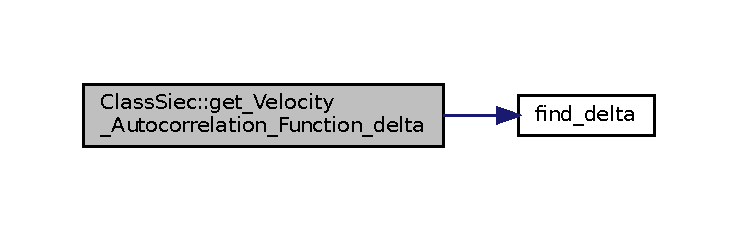
\includegraphics[width=350pt]{classClassSiec_a21be4d09c7aa47a5d3f216509ad5feef_cgraph}
\end{center}
\end{figure}
\mbox{\Hypertarget{classClassSiec_af6d6dbab3224e645c67e6c7dd2e02378}\label{classClassSiec_af6d6dbab3224e645c67e6c7dd2e02378}} 
\index{Class\+Siec@{Class\+Siec}!get\+\_\+\+Velocity\+\_\+\+Autocorrelation\+\_\+\+Function\+\_\+delta\+\_\+ratio@{get\+\_\+\+Velocity\+\_\+\+Autocorrelation\+\_\+\+Function\+\_\+delta\+\_\+ratio}}
\index{get\+\_\+\+Velocity\+\_\+\+Autocorrelation\+\_\+\+Function\+\_\+delta\+\_\+ratio@{get\+\_\+\+Velocity\+\_\+\+Autocorrelation\+\_\+\+Function\+\_\+delta\+\_\+ratio}!Class\+Siec@{Class\+Siec}}
\subsubsection{\texorpdfstring{get\+\_\+\+Velocity\+\_\+\+Autocorrelation\+\_\+\+Function\+\_\+delta\+\_\+ratio()}{get\_Velocity\_Autocorrelation\_Function\_delta\_ratio()}}
{\footnotesize\ttfamily double Class\+Siec\+::get\+\_\+\+Velocity\+\_\+\+Autocorrelation\+\_\+\+Function\+\_\+delta\+\_\+ratio (\begin{DoxyParamCaption}\item[{void}]{ }\end{DoxyParamCaption})}

Get Velocity Autocorrelation Function delta ratio \begin{DoxyReturn}{Returns}

\end{DoxyReturn}


Definition at line 1449 of file Class\+Siec.\+cpp.



References find\+\_\+delta(), and get\+\_\+\+Velocity\+\_\+\+Autocorrelation\+\_\+\+Function().

Here is the call graph for this function\+:
\nopagebreak
\begin{figure}[H]
\begin{center}
\leavevmode
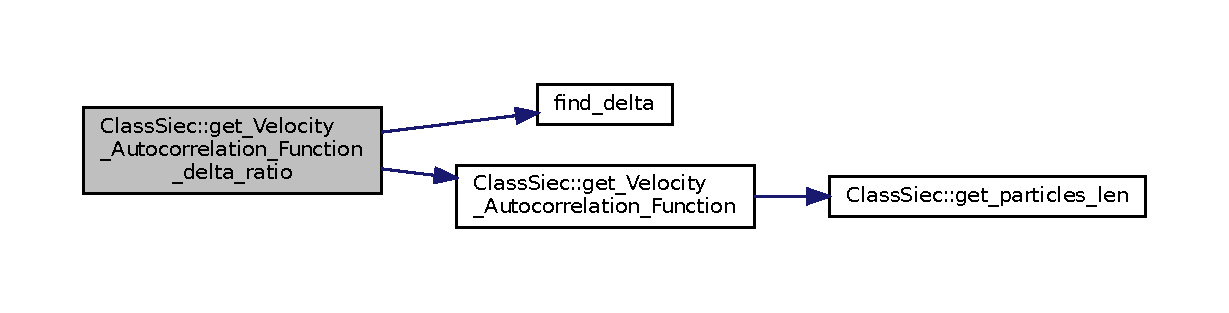
\includegraphics[width=350pt]{classClassSiec_af6d6dbab3224e645c67e6c7dd2e02378_cgraph}
\end{center}
\end{figure}
\mbox{\Hypertarget{classClassSiec_a5c2c133544d66df25e8b13e6b710272e}\label{classClassSiec_a5c2c133544d66df25e8b13e6b710272e}} 
\index{Class\+Siec@{Class\+Siec}!init@{init}}
\index{init@{init}!Class\+Siec@{Class\+Siec}}
\subsubsection{\texorpdfstring{init()}{init()}}
{\footnotesize\ttfamily int Class\+Siec\+::init (\begin{DoxyParamCaption}\item[{std\+::string}]{filename }\end{DoxyParamCaption})}


\begin{DoxyParams}{Parameters}
{\em filename} & \\
\hline
\end{DoxyParams}
\begin{DoxyReturn}{Returns}

\end{DoxyReturn}


Definition at line 953 of file Class\+Siec.\+cpp.



References get\+\_\+box\+\_\+info\+\_\+title(), OK, and set\+\_\+particles\+\_\+zero\+\_\+time().



Referenced by main().

Here is the call graph for this function\+:
\nopagebreak
\begin{figure}[H]
\begin{center}
\leavevmode
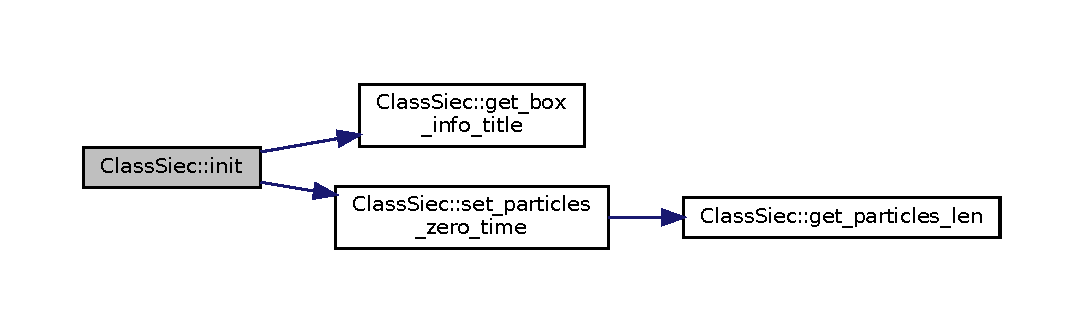
\includegraphics[width=350pt]{classClassSiec_a5c2c133544d66df25e8b13e6b710272e_cgraph}
\end{center}
\end{figure}
\mbox{\Hypertarget{classClassSiec_ab49b9f6b28f5e3c319384f518042272a}\label{classClassSiec_ab49b9f6b28f5e3c319384f518042272a}} 
\index{Class\+Siec@{Class\+Siec}!insert\+\_\+to\+\_\+file@{insert\+\_\+to\+\_\+file}}
\index{insert\+\_\+to\+\_\+file@{insert\+\_\+to\+\_\+file}!Class\+Siec@{Class\+Siec}}
\subsubsection{\texorpdfstring{insert\+\_\+to\+\_\+file()}{insert\_to\_file()}}
{\footnotesize\ttfamily int Class\+Siec\+::insert\+\_\+to\+\_\+file (\begin{DoxyParamCaption}\item[{std\+::string}]{data }\end{DoxyParamCaption})}

Flush string to file 
\begin{DoxyParams}{Parameters}
{\em data} & \\
\hline
\end{DoxyParams}
\begin{DoxyReturn}{Returns}

\end{DoxyReturn}


Definition at line 972 of file Class\+Siec.\+cpp.



References OK.



Referenced by main(), save\+\_\+\+R\+D\+F(), and step\+\_\+all().

\mbox{\Hypertarget{classClassSiec_a984c7c1d77c9cf78b6254529088028a4}\label{classClassSiec_a984c7c1d77c9cf78b6254529088028a4}} 
\index{Class\+Siec@{Class\+Siec}!save\+\_\+\+R\+DF@{save\+\_\+\+R\+DF}}
\index{save\+\_\+\+R\+DF@{save\+\_\+\+R\+DF}!Class\+Siec@{Class\+Siec}}
\subsubsection{\texorpdfstring{save\+\_\+\+R\+D\+F()}{save\_RDF()}}
{\footnotesize\ttfamily int Class\+Siec\+::save\+\_\+\+R\+DF (\begin{DoxyParamCaption}\item[{uint64\+\_\+t}]{prec = {\ttfamily 100},  }\item[{std\+::string}]{sep = {\ttfamily \char`\"{}~\char`\"{}} }\end{DoxyParamCaption})}

Save default R\+DF to file 
\begin{DoxyParams}{Parameters}
{\em prec} & \\
\hline
{\em sep} & \\
\hline
\end{DoxyParams}
\begin{DoxyReturn}{Returns}

\end{DoxyReturn}


Definition at line 1678 of file Class\+Siec.\+cpp.



References current\+\_\+\+R\+DF, get\+\_\+particles\+\_\+len(), insert\+\_\+to\+\_\+file(), OK, and thread\+\_\+\+R\+D\+F().

Here is the call graph for this function\+:
\nopagebreak
\begin{figure}[H]
\begin{center}
\leavevmode
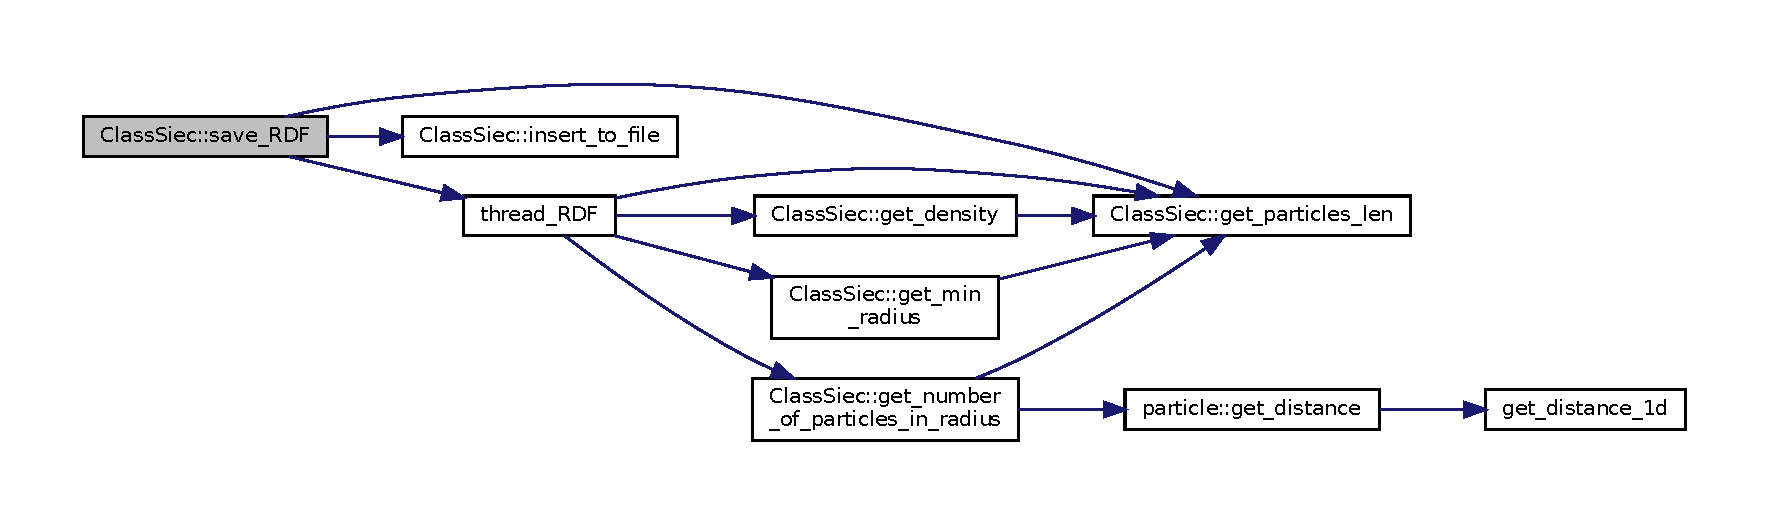
\includegraphics[width=350pt]{classClassSiec_a984c7c1d77c9cf78b6254529088028a4_cgraph}
\end{center}
\end{figure}
\mbox{\Hypertarget{classClassSiec_a9c96b5d39e27f8f2bdda6fd60113ceb6}\label{classClassSiec_a9c96b5d39e27f8f2bdda6fd60113ceb6}} 
\index{Class\+Siec@{Class\+Siec}!save\+\_\+\+R\+D\+F\+\_\+to\+\_\+array@{save\+\_\+\+R\+D\+F\+\_\+to\+\_\+array}}
\index{save\+\_\+\+R\+D\+F\+\_\+to\+\_\+array@{save\+\_\+\+R\+D\+F\+\_\+to\+\_\+array}!Class\+Siec@{Class\+Siec}}
\subsubsection{\texorpdfstring{save\+\_\+\+R\+D\+F\+\_\+to\+\_\+array()}{save\_RDF\_to\_array()}}
{\footnotesize\ttfamily void Class\+Siec\+::save\+\_\+\+R\+D\+F\+\_\+to\+\_\+array (\begin{DoxyParamCaption}\item[{vector$<$ double $>$ $\ast$}]{array,  }\item[{uint64\+\_\+t}]{prec = {\ttfamily 100} }\end{DoxyParamCaption})}



Definition at line 1711 of file Class\+Siec.\+cpp.



References current\+\_\+\+R\+DF, get\+\_\+particles\+\_\+len(), and thread\+\_\+\+R\+D\+F().



Referenced by main().

Here is the call graph for this function\+:
\nopagebreak
\begin{figure}[H]
\begin{center}
\leavevmode
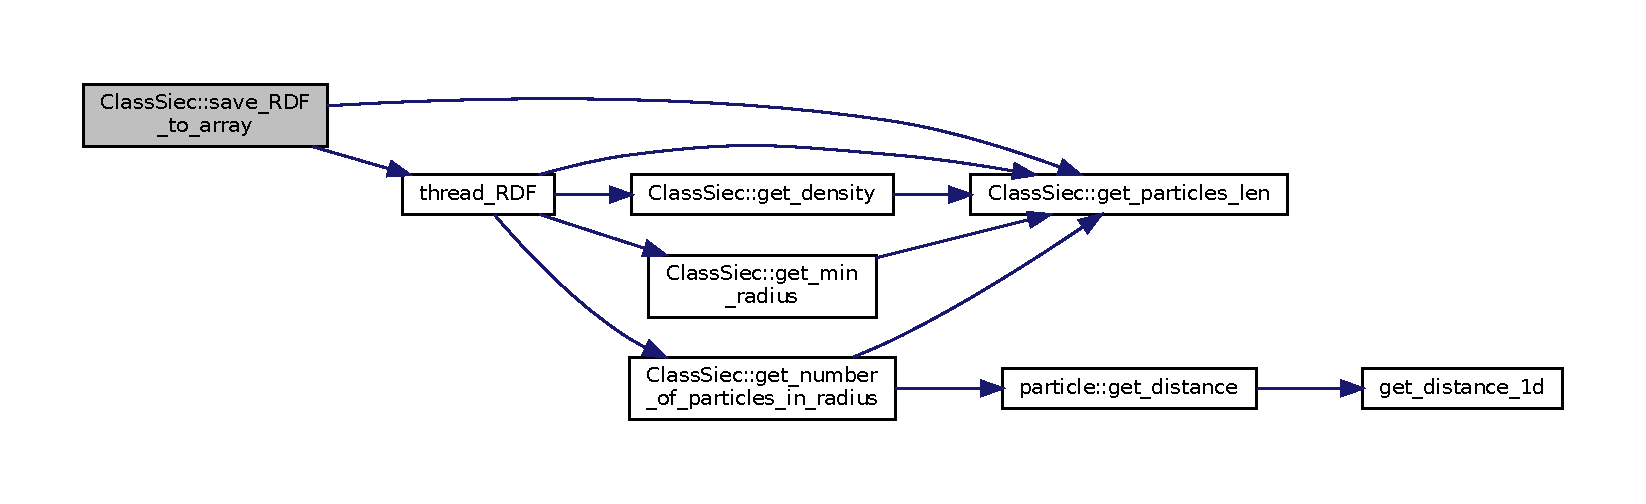
\includegraphics[width=350pt]{classClassSiec_a9c96b5d39e27f8f2bdda6fd60113ceb6_cgraph}
\end{center}
\end{figure}
\mbox{\Hypertarget{classClassSiec_a2ef8ae6a08683c8ed1c4e9d89b79e08e}\label{classClassSiec_a2ef8ae6a08683c8ed1c4e9d89b79e08e}} 
\index{Class\+Siec@{Class\+Siec}!set\+\_\+dt@{set\+\_\+dt}}
\index{set\+\_\+dt@{set\+\_\+dt}!Class\+Siec@{Class\+Siec}}
\subsubsection{\texorpdfstring{set\+\_\+dt()}{set\_dt()}}
{\footnotesize\ttfamily int Class\+Siec\+::set\+\_\+dt (\begin{DoxyParamCaption}\item[{double}]{dt }\end{DoxyParamCaption})}

Set delta time \begin{DoxyRefDesc}{Todo}
\item[\mbox{\hyperlink{todo__todo000002}{Todo}}]function is deprecated \end{DoxyRefDesc}

\begin{DoxyParams}{Parameters}
{\em dt} & \\
\hline
\end{DoxyParams}
\begin{DoxyReturn}{Returns}

\end{DoxyReturn}


Definition at line 394 of file Class\+Siec.\+cpp.



References OK.

\mbox{\Hypertarget{classClassSiec_a2adaa0e7fe44a2a68b7eba11c52d21bd}\label{classClassSiec_a2adaa0e7fe44a2a68b7eba11c52d21bd}} 
\index{Class\+Siec@{Class\+Siec}!set\+\_\+mass\+\_\+all@{set\+\_\+mass\+\_\+all}}
\index{set\+\_\+mass\+\_\+all@{set\+\_\+mass\+\_\+all}!Class\+Siec@{Class\+Siec}}
\subsubsection{\texorpdfstring{set\+\_\+mass\+\_\+all()}{set\_mass\_all()}}
{\footnotesize\ttfamily int Class\+Siec\+::set\+\_\+mass\+\_\+all (\begin{DoxyParamCaption}\item[{double}]{mass = {\ttfamily 1.0} }\end{DoxyParamCaption})}

Sets the masses for all particles 
\begin{DoxyParams}{Parameters}
{\em mass} & \\
\hline
\end{DoxyParams}
\begin{DoxyReturn}{Returns}

\end{DoxyReturn}


Definition at line 745 of file Class\+Siec.\+cpp.



References get\+\_\+particles\+\_\+len(), OK, and particles.



Referenced by main().

Here is the call graph for this function\+:
\nopagebreak
\begin{figure}[H]
\begin{center}
\leavevmode
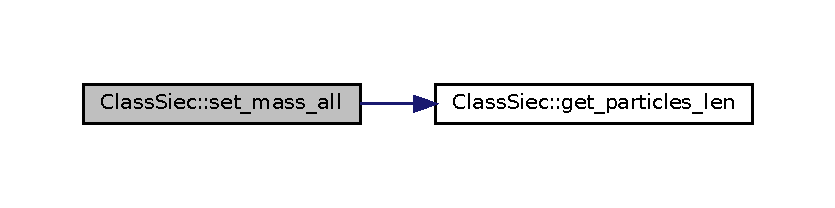
\includegraphics[width=350pt]{classClassSiec_a2adaa0e7fe44a2a68b7eba11c52d21bd_cgraph}
\end{center}
\end{figure}
\mbox{\Hypertarget{classClassSiec_aa2eff85fe7fc842b2d0631118d533154}\label{classClassSiec_aa2eff85fe7fc842b2d0631118d533154}} 
\index{Class\+Siec@{Class\+Siec}!set\+\_\+mass\+\_\+to\+\_\+area@{set\+\_\+mass\+\_\+to\+\_\+area}}
\index{set\+\_\+mass\+\_\+to\+\_\+area@{set\+\_\+mass\+\_\+to\+\_\+area}!Class\+Siec@{Class\+Siec}}
\subsubsection{\texorpdfstring{set\+\_\+mass\+\_\+to\+\_\+area()}{set\_mass\_to\_area()}}
{\footnotesize\ttfamily int Class\+Siec\+::set\+\_\+mass\+\_\+to\+\_\+area (\begin{DoxyParamCaption}\item[{double}]{ratio = {\ttfamily 1.0} }\end{DoxyParamCaption})}

Sets the masses according to the area of particle 
\begin{DoxyParams}{Parameters}
{\em ratio} & \\
\hline
\end{DoxyParams}
\begin{DoxyReturn}{Returns}

\end{DoxyReturn}


Definition at line 730 of file Class\+Siec.\+cpp.



References get\+\_\+particles\+\_\+len(), OK, and particles.

Here is the call graph for this function\+:
\nopagebreak
\begin{figure}[H]
\begin{center}
\leavevmode
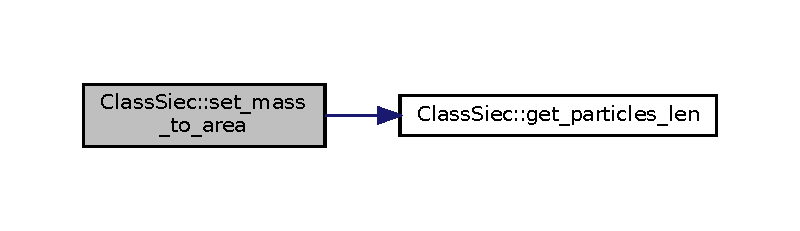
\includegraphics[width=350pt]{classClassSiec_aa2eff85fe7fc842b2d0631118d533154_cgraph}
\end{center}
\end{figure}
\mbox{\Hypertarget{classClassSiec_a361b139e9734e15599847d2060d85d6b}\label{classClassSiec_a361b139e9734e15599847d2060d85d6b}} 
\index{Class\+Siec@{Class\+Siec}!set\+\_\+mass\+\_\+to\+\_\+radius@{set\+\_\+mass\+\_\+to\+\_\+radius}}
\index{set\+\_\+mass\+\_\+to\+\_\+radius@{set\+\_\+mass\+\_\+to\+\_\+radius}!Class\+Siec@{Class\+Siec}}
\subsubsection{\texorpdfstring{set\+\_\+mass\+\_\+to\+\_\+radius()}{set\_mass\_to\_radius()}}
{\footnotesize\ttfamily int Class\+Siec\+::set\+\_\+mass\+\_\+to\+\_\+radius (\begin{DoxyParamCaption}\item[{double}]{ratio = {\ttfamily 1.0} }\end{DoxyParamCaption})}

Sets the masses according to the radius of particle 
\begin{DoxyParams}{Parameters}
{\em ratio} & \\
\hline
\end{DoxyParams}
\begin{DoxyReturn}{Returns}

\end{DoxyReturn}


Definition at line 716 of file Class\+Siec.\+cpp.



References get\+\_\+particles\+\_\+len(), OK, and particles.

Here is the call graph for this function\+:
\nopagebreak
\begin{figure}[H]
\begin{center}
\leavevmode
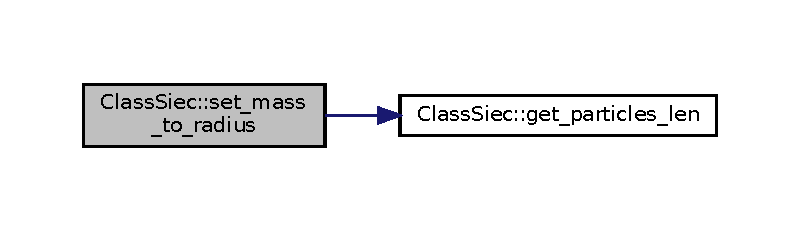
\includegraphics[width=350pt]{classClassSiec_a361b139e9734e15599847d2060d85d6b_cgraph}
\end{center}
\end{figure}
\mbox{\Hypertarget{classClassSiec_ab2a445e522e2d8c59177fd28c074c1c1}\label{classClassSiec_ab2a445e522e2d8c59177fd28c074c1c1}} 
\index{Class\+Siec@{Class\+Siec}!set\+\_\+momentum\+\_\+to\+\_\+zero@{set\+\_\+momentum\+\_\+to\+\_\+zero}}
\index{set\+\_\+momentum\+\_\+to\+\_\+zero@{set\+\_\+momentum\+\_\+to\+\_\+zero}!Class\+Siec@{Class\+Siec}}
\subsubsection{\texorpdfstring{set\+\_\+momentum\+\_\+to\+\_\+zero()}{set\_momentum\_to\_zero()}}
{\footnotesize\ttfamily int Class\+Siec\+::set\+\_\+momentum\+\_\+to\+\_\+zero (\begin{DoxyParamCaption}\item[{double}]{temperature,  }\item[{double}]{precision = {\ttfamily 0.001} }\end{DoxyParamCaption})}

Set temperature to Ekpoz\+\_\+t 
\begin{DoxyParams}{Parameters}
{\em Ekpoz\+\_\+t} & \\
\hline
{\em precision} & \\
\hline
\end{DoxyParams}
\begin{DoxyReturn}{Returns}

\end{DoxyReturn}


Definition at line 760 of file Class\+Siec.\+cpp.



References find\+\_\+is\+\_\+in\+\_\+range(), get\+\_\+kinetic\+\_\+energy(), get\+\_\+particles\+\_\+len(), get\+\_\+temperature(), OK, and particles.



Referenced by main().

Here is the call graph for this function\+:
\nopagebreak
\begin{figure}[H]
\begin{center}
\leavevmode
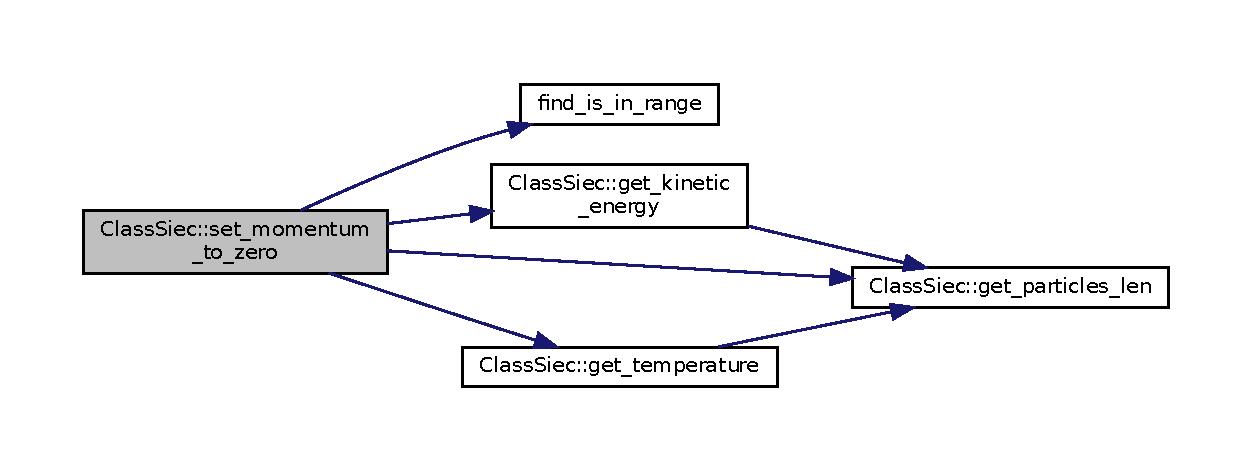
\includegraphics[width=350pt]{classClassSiec_ab2a445e522e2d8c59177fd28c074c1c1_cgraph}
\end{center}
\end{figure}
\mbox{\Hypertarget{classClassSiec_a37811fccdbeb4119061a02cfb9386677}\label{classClassSiec_a37811fccdbeb4119061a02cfb9386677}} 
\index{Class\+Siec@{Class\+Siec}!set\+\_\+particles\+\_\+zero\+\_\+time@{set\+\_\+particles\+\_\+zero\+\_\+time}}
\index{set\+\_\+particles\+\_\+zero\+\_\+time@{set\+\_\+particles\+\_\+zero\+\_\+time}!Class\+Siec@{Class\+Siec}}
\subsubsection{\texorpdfstring{set\+\_\+particles\+\_\+zero\+\_\+time()}{set\_particles\_zero\_time()}}
{\footnotesize\ttfamily int Class\+Siec\+::set\+\_\+particles\+\_\+zero\+\_\+time (\begin{DoxyParamCaption}\item[{void}]{ }\end{DoxyParamCaption})}

Saves the initial states to an individual array \begin{DoxyReturn}{Returns}

\end{DoxyReturn}


Definition at line 806 of file Class\+Siec.\+cpp.



References get\+\_\+particles\+\_\+len(), OK, particles, and particles\+\_\+zero\+\_\+time.



Referenced by init(), and main().

Here is the call graph for this function\+:
\nopagebreak
\begin{figure}[H]
\begin{center}
\leavevmode
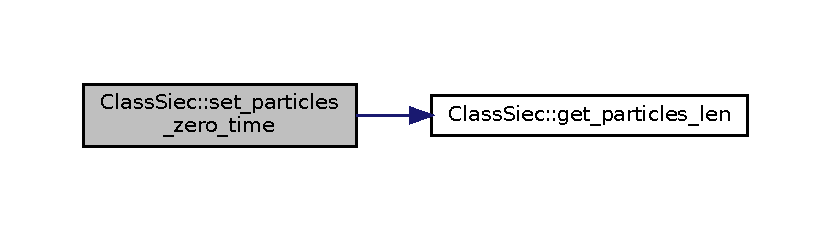
\includegraphics[width=350pt]{classClassSiec_a37811fccdbeb4119061a02cfb9386677_cgraph}
\end{center}
\end{figure}
\mbox{\Hypertarget{classClassSiec_a4b63c475330f7b0c96a244f55a624fac}\label{classClassSiec_a4b63c475330f7b0c96a244f55a624fac}} 
\index{Class\+Siec@{Class\+Siec}!set\+\_\+random\+\_\+size@{set\+\_\+random\+\_\+size}}
\index{set\+\_\+random\+\_\+size@{set\+\_\+random\+\_\+size}!Class\+Siec@{Class\+Siec}}
\subsubsection{\texorpdfstring{set\+\_\+random\+\_\+size()}{set\_random\_size()}}
{\footnotesize\ttfamily int Class\+Siec\+::set\+\_\+random\+\_\+size (\begin{DoxyParamCaption}\item[{double}]{min,  }\item[{double}]{max }\end{DoxyParamCaption})}

Set random size of particles 
\begin{DoxyParams}{Parameters}
{\em min} & \\
\hline
{\em max} & \\
\hline
\end{DoxyParams}
\begin{DoxyReturn}{Returns}

\end{DoxyReturn}


Definition at line 692 of file Class\+Siec.\+cpp.



References E\+R\+R\+OR, get\+\_\+particles\+\_\+len(), OK, and particles.

Here is the call graph for this function\+:
\nopagebreak
\begin{figure}[H]
\begin{center}
\leavevmode
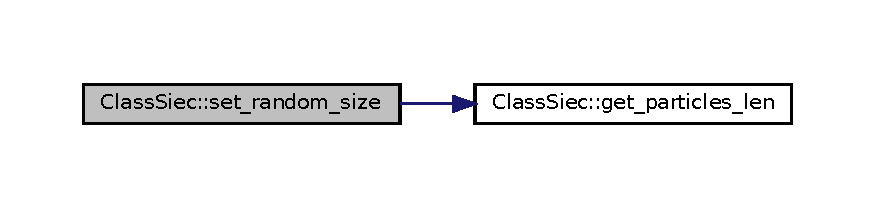
\includegraphics[width=350pt]{classClassSiec_a4b63c475330f7b0c96a244f55a624fac_cgraph}
\end{center}
\end{figure}
\mbox{\Hypertarget{classClassSiec_a29968ccc2e9318ca89ae0b3dac4a390d}\label{classClassSiec_a29968ccc2e9318ca89ae0b3dac4a390d}} 
\index{Class\+Siec@{Class\+Siec}!set\+\_\+random\+\_\+velocity@{set\+\_\+random\+\_\+velocity}}
\index{set\+\_\+random\+\_\+velocity@{set\+\_\+random\+\_\+velocity}!Class\+Siec@{Class\+Siec}}
\subsubsection{\texorpdfstring{set\+\_\+random\+\_\+velocity()}{set\_random\_velocity()}}
{\footnotesize\ttfamily int Class\+Siec\+::set\+\_\+random\+\_\+velocity (\begin{DoxyParamCaption}\item[{double}]{multiplier = {\ttfamily 1.0} }\end{DoxyParamCaption})}

Set random velocity for all particles 
\begin{DoxyParams}{Parameters}
{\em multiplier} & \\
\hline
\end{DoxyParams}
\begin{DoxyReturn}{Returns}

\end{DoxyReturn}


Definition at line 668 of file Class\+Siec.\+cpp.



References get\+\_\+particles\+\_\+len(), OK, and particles.



Referenced by main().

Here is the call graph for this function\+:
\nopagebreak
\begin{figure}[H]
\begin{center}
\leavevmode
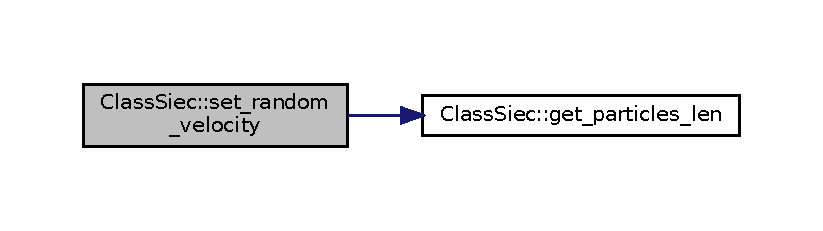
\includegraphics[width=350pt]{classClassSiec_a29968ccc2e9318ca89ae0b3dac4a390d_cgraph}
\end{center}
\end{figure}
\mbox{\Hypertarget{classClassSiec_a0de17762248441c53936ee7924776052}\label{classClassSiec_a0de17762248441c53936ee7924776052}} 
\index{Class\+Siec@{Class\+Siec}!step\+\_\+all@{step\+\_\+all}}
\index{step\+\_\+all@{step\+\_\+all}!Class\+Siec@{Class\+Siec}}
\subsubsection{\texorpdfstring{step\+\_\+all()}{step\_all()}}
{\footnotesize\ttfamily int Class\+Siec\+::step\+\_\+all (\begin{DoxyParamCaption}\item[{int}]{debug = {\ttfamily 0} }\end{DoxyParamCaption})}

Step all particles \begin{DoxyReturn}{Returns}

\end{DoxyReturn}


Definition at line 1001 of file Class\+Siec.\+cpp.



References box\+\_\+x, box\+\_\+y, particle\+::color, distance, distancex, distancey, fix\+\_\+position(), get\+\_\+box\+\_\+info(), get\+\_\+box\+\_\+info\+\_\+raw(), get\+\_\+min\+\_\+radius(), get\+\_\+next\+\_\+collision\+\_\+particles(), get\+\_\+particles\+\_\+len(), get\+\_\+radial\+\_\+distribution\+\_\+function(), particle\+::get\+\_\+velocity(), get\+\_\+\+Velocity\+\_\+\+Autocorrelation\+\_\+\+Function(), insert\+\_\+to\+\_\+file(), OK, particles, particle\+::pos, particle\+::t, th\+\_\+to\+\_\+box(), particle\+::vel, and zderzenie().



Referenced by main(), and thread\+\_\+siec().

Here is the call graph for this function\+:
\nopagebreak
\begin{figure}[H]
\begin{center}
\leavevmode
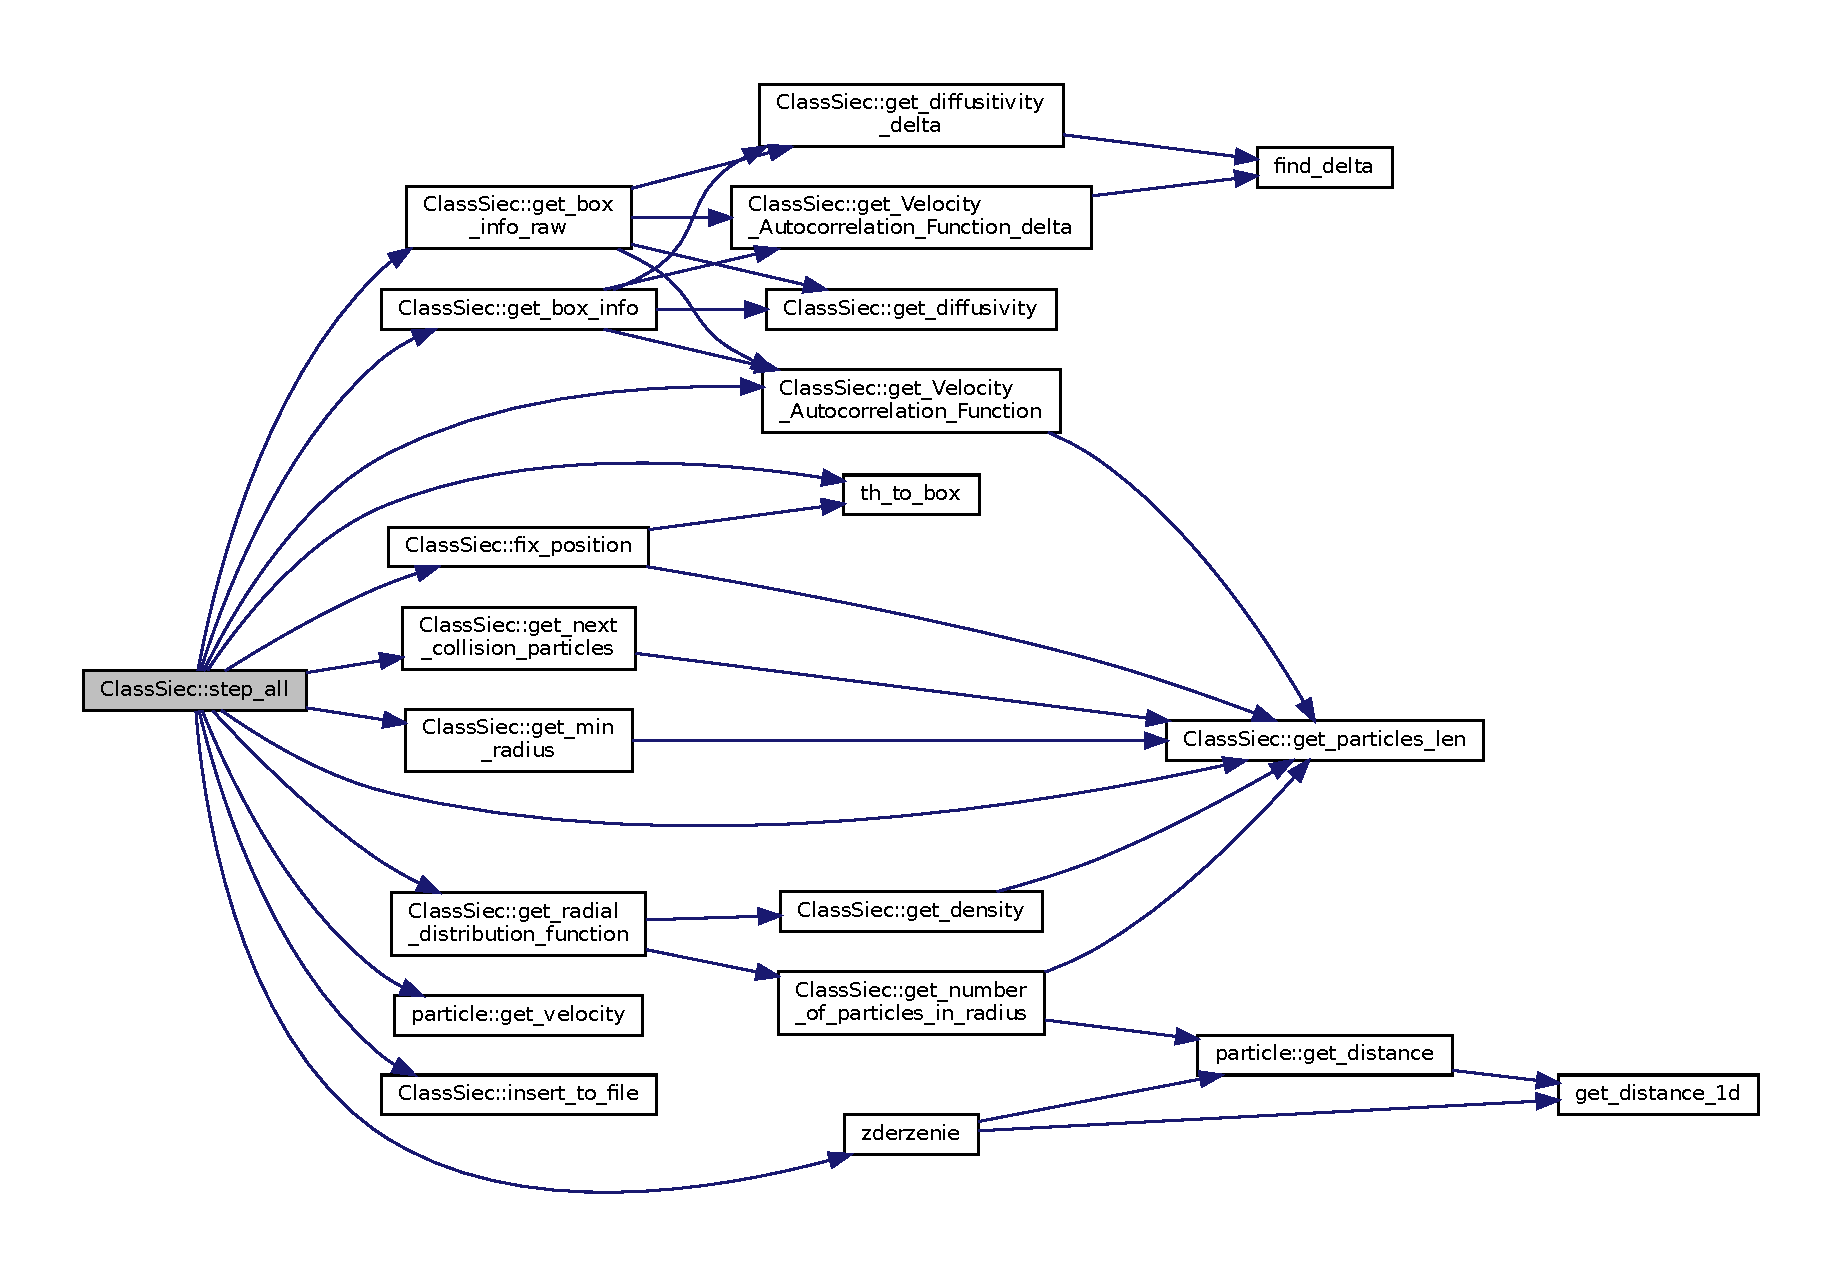
\includegraphics[width=350pt]{classClassSiec_a0de17762248441c53936ee7924776052_cgraph}
\end{center}
\end{figure}


\subsection{Member Data Documentation}
\mbox{\Hypertarget{classClassSiec_a8ebc9e2a0a8f7ccf4736482aa2a5f673}\label{classClassSiec_a8ebc9e2a0a8f7ccf4736482aa2a5f673}} 
\index{Class\+Siec@{Class\+Siec}!box\+\_\+x@{box\+\_\+x}}
\index{box\+\_\+x@{box\+\_\+x}!Class\+Siec@{Class\+Siec}}
\subsubsection{\texorpdfstring{box\+\_\+x}{box\_x}}
{\footnotesize\ttfamily double Class\+Siec\+::box\+\_\+x}



Definition at line 200 of file Class\+Siec.\+h.



Referenced by Class\+Siec(), convert\+\_\+to\+\_\+box(), create\+\_\+hexagonal(), create\+\_\+honeycomb(), create\+\_\+square(), fix\+\_\+position(), get\+\_\+box\+\_\+x(), get\+\_\+density(), get\+\_\+density\+\_\+real(), get\+\_\+next\+\_\+collision\+\_\+particle\+\_\+number(), get\+\_\+next\+\_\+collision\+\_\+particles(), get\+\_\+number\+\_\+of\+\_\+particles\+\_\+in\+\_\+radius(), get\+\_\+packing\+\_\+ratio(), get\+\_\+\+R\+D\+F\+\_\+r(), and step\+\_\+all().

\mbox{\Hypertarget{classClassSiec_a51b98a4d58f22b84e410eaf2c7b31c4b}\label{classClassSiec_a51b98a4d58f22b84e410eaf2c7b31c4b}} 
\index{Class\+Siec@{Class\+Siec}!box\+\_\+y@{box\+\_\+y}}
\index{box\+\_\+y@{box\+\_\+y}!Class\+Siec@{Class\+Siec}}
\subsubsection{\texorpdfstring{box\+\_\+y}{box\_y}}
{\footnotesize\ttfamily double Class\+Siec\+::box\+\_\+y}



Definition at line 201 of file Class\+Siec.\+h.



Referenced by Class\+Siec(), convert\+\_\+to\+\_\+box(), create\+\_\+hexagonal(), create\+\_\+honeycomb(), create\+\_\+square(), fix\+\_\+position(), get\+\_\+box\+\_\+y(), get\+\_\+density(), get\+\_\+density\+\_\+real(), get\+\_\+next\+\_\+collision\+\_\+particle\+\_\+number(), get\+\_\+next\+\_\+collision\+\_\+particles(), get\+\_\+number\+\_\+of\+\_\+particles\+\_\+in\+\_\+radius(), get\+\_\+packing\+\_\+ratio(), get\+\_\+\+R\+D\+F\+\_\+r(), and step\+\_\+all().

\mbox{\Hypertarget{classClassSiec_aaa4641c3eb550d26c64a785729e8cd63}\label{classClassSiec_aaa4641c3eb550d26c64a785729e8cd63}} 
\index{Class\+Siec@{Class\+Siec}!current\+\_\+\+R\+DF@{current\+\_\+\+R\+DF}}
\index{current\+\_\+\+R\+DF@{current\+\_\+\+R\+DF}!Class\+Siec@{Class\+Siec}}
\subsubsection{\texorpdfstring{current\+\_\+\+R\+DF}{current\_RDF}}
{\footnotesize\ttfamily vector$<$double$>$ Class\+Siec\+::current\+\_\+\+R\+DF}



Definition at line 196 of file Class\+Siec.\+h.



Referenced by draw\+\_\+\+R\+D\+F(), get\+\_\+radial\+\_\+distribution\+\_\+function(), save\+\_\+\+R\+D\+F(), save\+\_\+\+R\+D\+F\+\_\+to\+\_\+array(), and thread\+\_\+\+R\+D\+F().

\mbox{\Hypertarget{classClassSiec_a4593ac900fa92dd33f9b40010b35efb9}\label{classClassSiec_a4593ac900fa92dd33f9b40010b35efb9}} 
\index{Class\+Siec@{Class\+Siec}!distance@{distance}}
\index{distance@{distance}!Class\+Siec@{Class\+Siec}}
\subsubsection{\texorpdfstring{distance}{distance}}
{\footnotesize\ttfamily double Class\+Siec\+::distance}



Definition at line 199 of file Class\+Siec.\+h.



Referenced by step\+\_\+all().

\mbox{\Hypertarget{classClassSiec_a98e9ee22a2e12ce6612d1ce6e785cda2}\label{classClassSiec_a98e9ee22a2e12ce6612d1ce6e785cda2}} 
\index{Class\+Siec@{Class\+Siec}!distancex@{distancex}}
\index{distancex@{distancex}!Class\+Siec@{Class\+Siec}}
\subsubsection{\texorpdfstring{distancex}{distancex}}
{\footnotesize\ttfamily double Class\+Siec\+::distancex}



Definition at line 197 of file Class\+Siec.\+h.



Referenced by step\+\_\+all().

\mbox{\Hypertarget{classClassSiec_a5c100f779c613f9c747b0b7a3f02f2d9}\label{classClassSiec_a5c100f779c613f9c747b0b7a3f02f2d9}} 
\index{Class\+Siec@{Class\+Siec}!distancey@{distancey}}
\index{distancey@{distancey}!Class\+Siec@{Class\+Siec}}
\subsubsection{\texorpdfstring{distancey}{distancey}}
{\footnotesize\ttfamily double Class\+Siec\+::distancey}



Definition at line 198 of file Class\+Siec.\+h.



Referenced by step\+\_\+all().

\mbox{\Hypertarget{classClassSiec_aa1a11eee47b10c11930952f092110e94}\label{classClassSiec_aa1a11eee47b10c11930952f092110e94}} 
\index{Class\+Siec@{Class\+Siec}!particles@{particles}}
\index{particles@{particles}!Class\+Siec@{Class\+Siec}}
\subsubsection{\texorpdfstring{particles}{particles}}
{\footnotesize\ttfamily vector$<$\mbox{\hyperlink{structparticle}{particle}}$>$ Class\+Siec\+::particles}



Definition at line 194 of file Class\+Siec.\+h.



Referenced by add\+\_\+particle(), create\+\_\+hexagonal(), create\+\_\+honeycomb(), draw\+\_\+all(), fix\+\_\+position(), get\+\_\+density\+\_\+real(), get\+\_\+kinetic\+\_\+energy(), get\+\_\+max\+\_\+radius(), get\+\_\+min\+\_\+radius(), get\+\_\+next\+\_\+collision\+\_\+particle\+\_\+number(), get\+\_\+next\+\_\+collision\+\_\+particles(), get\+\_\+number\+\_\+of\+\_\+particles\+\_\+in\+\_\+radius(), get\+\_\+packing\+\_\+ratio(), get\+\_\+particle(), get\+\_\+particles\+\_\+len(), get\+\_\+\+R\+D\+F\+\_\+r(), get\+\_\+temperature(), get\+\_\+\+Velocity\+\_\+\+Autocorrelation\+\_\+\+Function(), set\+\_\+mass\+\_\+all(), set\+\_\+mass\+\_\+to\+\_\+area(), set\+\_\+mass\+\_\+to\+\_\+radius(), set\+\_\+momentum\+\_\+to\+\_\+zero(), set\+\_\+particles\+\_\+zero\+\_\+time(), set\+\_\+random\+\_\+size(), set\+\_\+random\+\_\+velocity(), step\+\_\+all(), thread\+\_\+\+R\+D\+F(), and $\sim$\+Class\+Siec().

\mbox{\Hypertarget{classClassSiec_aa1096135e230dbae78ec05efc8a4725f}\label{classClassSiec_aa1096135e230dbae78ec05efc8a4725f}} 
\index{Class\+Siec@{Class\+Siec}!particles\+\_\+zero\+\_\+time@{particles\+\_\+zero\+\_\+time}}
\index{particles\+\_\+zero\+\_\+time@{particles\+\_\+zero\+\_\+time}!Class\+Siec@{Class\+Siec}}
\subsubsection{\texorpdfstring{particles\+\_\+zero\+\_\+time}{particles\_zero\_time}}
{\footnotesize\ttfamily vector$<$\mbox{\hyperlink{structparticle__zero__time}{particle\+\_\+zero\+\_\+time}}$>$ Class\+Siec\+::particles\+\_\+zero\+\_\+time}



Definition at line 195 of file Class\+Siec.\+h.



Referenced by get\+\_\+\+Velocity\+\_\+\+Autocorrelation\+\_\+\+Function(), and set\+\_\+particles\+\_\+zero\+\_\+time().



The documentation for this class was generated from the following files\+:\begin{DoxyCompactItemize}
\item 
\mbox{\hyperlink{ClassSiec_8h}{Class\+Siec.\+h}}\item 
\mbox{\hyperlink{ClassSiec_8cpp}{Class\+Siec.\+cpp}}\end{DoxyCompactItemize}

\hypertarget{structpart__particles}{}\section{part\+\_\+particles Struct Reference}
\label{structpart__particles}\index{part\+\_\+particles@{part\+\_\+particles}}


{\ttfamily \#include $<$Class\+Siec.\+h$>$}



Collaboration diagram for part\+\_\+particles\+:\nopagebreak
\begin{figure}[H]
\begin{center}
\leavevmode
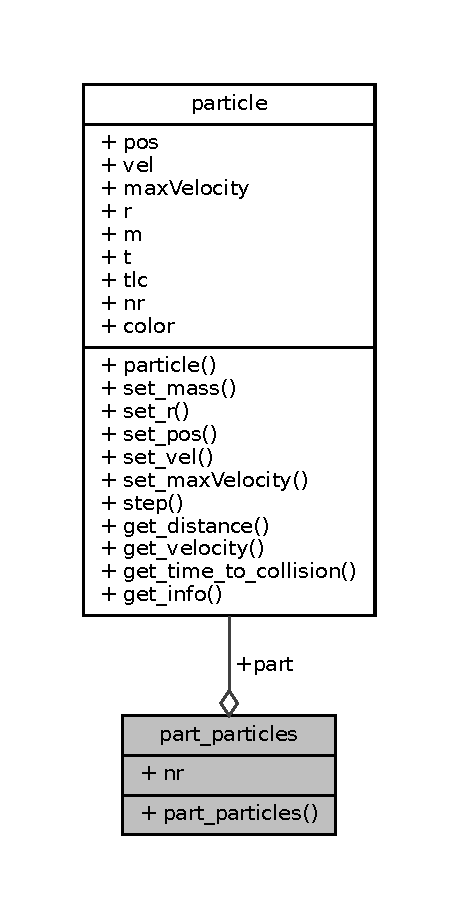
\includegraphics[width=220pt]{structpart__particles__coll__graph}
\end{center}
\end{figure}
\subsection*{Public Member Functions}
\begin{DoxyCompactItemize}
\item 
\mbox{\hyperlink{structpart__particles_a8e512b2ab1f29f2d2f11921b1328b4c4}{part\+\_\+particles}} (\mbox{\hyperlink{structparticle}{particle}} \mbox{\hyperlink{structpart__particles_a0f382b0ca436a15a067fdd4086d6e55c}{part}}, uint64\+\_\+t \mbox{\hyperlink{structpart__particles_ae596ac143f70897619e591081481c731}{nr}})
\end{DoxyCompactItemize}
\subsection*{Public Attributes}
\begin{DoxyCompactItemize}
\item 
\mbox{\hyperlink{structparticle}{particle}} \mbox{\hyperlink{structpart__particles_a0f382b0ca436a15a067fdd4086d6e55c}{part}}
\item 
uint64\+\_\+t \mbox{\hyperlink{structpart__particles_ae596ac143f70897619e591081481c731}{nr}}
\end{DoxyCompactItemize}


\subsection{Detailed Description}


Definition at line 69 of file Class\+Siec.\+h.



\subsection{Constructor \& Destructor Documentation}
\mbox{\Hypertarget{structpart__particles_a8e512b2ab1f29f2d2f11921b1328b4c4}\label{structpart__particles_a8e512b2ab1f29f2d2f11921b1328b4c4}} 
\index{part\+\_\+particles@{part\+\_\+particles}!part\+\_\+particles@{part\+\_\+particles}}
\index{part\+\_\+particles@{part\+\_\+particles}!part\+\_\+particles@{part\+\_\+particles}}
\subsubsection{\texorpdfstring{part\+\_\+particles()}{part\_particles()}}
{\footnotesize\ttfamily part\+\_\+particles\+::part\+\_\+particles (\begin{DoxyParamCaption}\item[{\mbox{\hyperlink{structparticle}{particle}}}]{part,  }\item[{uint64\+\_\+t}]{nr }\end{DoxyParamCaption})}



\subsection{Member Data Documentation}
\mbox{\Hypertarget{structpart__particles_ae596ac143f70897619e591081481c731}\label{structpart__particles_ae596ac143f70897619e591081481c731}} 
\index{part\+\_\+particles@{part\+\_\+particles}!nr@{nr}}
\index{nr@{nr}!part\+\_\+particles@{part\+\_\+particles}}
\subsubsection{\texorpdfstring{nr}{nr}}
{\footnotesize\ttfamily uint64\+\_\+t part\+\_\+particles\+::nr}



Definition at line 73 of file Class\+Siec.\+h.

\mbox{\Hypertarget{structpart__particles_a0f382b0ca436a15a067fdd4086d6e55c}\label{structpart__particles_a0f382b0ca436a15a067fdd4086d6e55c}} 
\index{part\+\_\+particles@{part\+\_\+particles}!part@{part}}
\index{part@{part}!part\+\_\+particles@{part\+\_\+particles}}
\subsubsection{\texorpdfstring{part}{part}}
{\footnotesize\ttfamily \mbox{\hyperlink{structparticle}{particle}} part\+\_\+particles\+::part}



Definition at line 72 of file Class\+Siec.\+h.



The documentation for this struct was generated from the following file\+:\begin{DoxyCompactItemize}
\item 
\mbox{\hyperlink{ClassSiec_8h}{Class\+Siec.\+h}}\end{DoxyCompactItemize}

\hypertarget{structparticle}{}\section{particle Struct Reference}
\label{structparticle}\index{particle@{particle}}


{\ttfamily \#include $<$Class\+Siec.\+h$>$}



Collaboration diagram for particle\+:\nopagebreak
\begin{figure}[H]
\begin{center}
\leavevmode
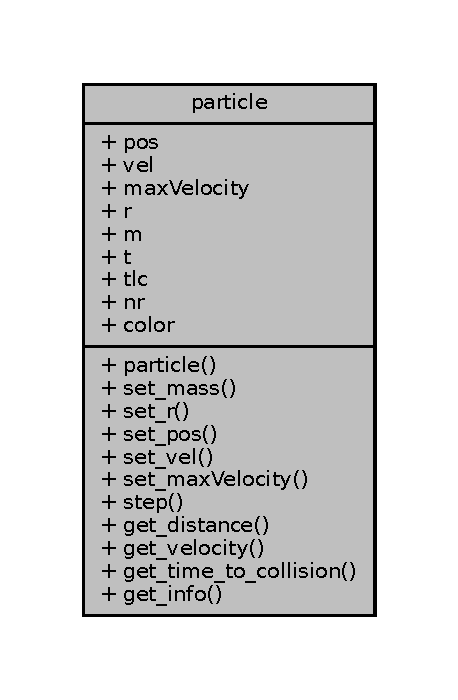
\includegraphics[width=220pt]{structparticle__coll__graph}
\end{center}
\end{figure}
\subsection*{Public Member Functions}
\begin{DoxyCompactItemize}
\item 
\mbox{\hyperlink{structparticle_a747b2142fefd6da08d95d84b32d985c5}{particle}} (double x, double y, double \mbox{\hyperlink{structparticle_a9ba64d6fa0d4bda34688d54a05341b77}{r}}, double vx=0.\+0, double vy=0.\+0, double \mbox{\hyperlink{structparticle_a2ea1a35ec678df5cc776dfd6bd377fad}{max\+Velocity}}=0.\+0, uint64\+\_\+t \mbox{\hyperlink{structparticle_a055d478842e85c5f730fc75f16254852}{nr}}=0)
\item 
int \mbox{\hyperlink{structparticle_af0c523c22c7b51a1a932f5f3f30b24a3}{set\+\_\+mass}} (double \mbox{\hyperlink{structparticle_a4cb4f184e6cd2b5dc0dc555d14f265dd}{m}})
\item 
int \mbox{\hyperlink{structparticle_ad45d7067a63de0b6c6ce07723a8e7be2}{set\+\_\+r}} (double \mbox{\hyperlink{structparticle_a9ba64d6fa0d4bda34688d54a05341b77}{r}})
\item 
int \mbox{\hyperlink{structparticle_a1088eb89ce4d29bc645160b91ba328c3}{set\+\_\+pos}} (double x, double y)
\item 
int \mbox{\hyperlink{structparticle_aafcf36063e5b6b0719b7ee8377f3c880}{set\+\_\+vel}} (double vx, double vy)
\item 
int \mbox{\hyperlink{structparticle_a842a75343ebbcdcaf53e95f0f1286d9a}{set\+\_\+max\+Velocity}} (double \mbox{\hyperlink{structparticle_a2ea1a35ec678df5cc776dfd6bd377fad}{max\+Velocity}})
\item 
int \mbox{\hyperlink{structparticle_a4f06bd4316643ca9ba721a4f768763a6}{step}} (double dt=1.\+0)
\item 
double \mbox{\hyperlink{structparticle_ab28d2ff9718bfa0fb801275d90f36a9d}{get\+\_\+distance}} (\mbox{\hyperlink{structparticle}{particle}} $\ast$to\+\_\+particle, double box\+\_\+x=0.\+0, double box\+\_\+y=0.\+0)
\item 
double \mbox{\hyperlink{structparticle_a8ca7119317b6176296ba0e4a0734ee33}{get\+\_\+velocity}} (void)
\item 
double \mbox{\hyperlink{structparticle_a8075edc35cef018e8d5fabcce3bc099e}{get\+\_\+time\+\_\+to\+\_\+collision}} (\mbox{\hyperlink{structparticle}{particle}} $\ast$to\+\_\+particle, double box\+\_\+x=0.\+0, double box\+\_\+y=0.\+0)
\item 
std\+::string \mbox{\hyperlink{structparticle_a74457d580da5637e77c1d72ba7a31bb5}{get\+\_\+info}} (void)
\end{DoxyCompactItemize}
\subsection*{Public Attributes}
\begin{DoxyCompactItemize}
\item 
double \mbox{\hyperlink{structparticle_a9ba2ff9e556c82ec96f56ce659c1ad50}{pos}} \mbox{[}2\mbox{]}
\item 
double \mbox{\hyperlink{structparticle_abd12470a54dcbf5694c6adeb8c06ef8b}{vel}} \mbox{[}2\mbox{]}
\item 
double \mbox{\hyperlink{structparticle_a2ea1a35ec678df5cc776dfd6bd377fad}{max\+Velocity}}
\item 
double \mbox{\hyperlink{structparticle_a9ba64d6fa0d4bda34688d54a05341b77}{r}}
\item 
double \mbox{\hyperlink{structparticle_a4cb4f184e6cd2b5dc0dc555d14f265dd}{m}}
\item 
double \mbox{\hyperlink{structparticle_a5225483b35b28edcf29be553a367a952}{t}}
\item 
double \mbox{\hyperlink{structparticle_a5ab99949ec29f5623413672b923ffa25}{tlc}}
\item 
uint64\+\_\+t \mbox{\hyperlink{structparticle_a055d478842e85c5f730fc75f16254852}{nr}}
\item 
A\+L\+L\+E\+G\+R\+O\+\_\+\+C\+O\+L\+OR \mbox{\hyperlink{structparticle_a7ea0e8707e7e91c3f298c5881bce4581}{color}}
\end{DoxyCompactItemize}


\subsection{Detailed Description}


Definition at line 38 of file Class\+Siec.\+h.



\subsection{Constructor \& Destructor Documentation}
\mbox{\Hypertarget{structparticle_a747b2142fefd6da08d95d84b32d985c5}\label{structparticle_a747b2142fefd6da08d95d84b32d985c5}} 
\index{particle@{particle}!particle@{particle}}
\index{particle@{particle}!particle@{particle}}
\subsubsection{\texorpdfstring{particle()}{particle()}}
{\footnotesize\ttfamily particle\+::particle (\begin{DoxyParamCaption}\item[{double}]{x,  }\item[{double}]{y,  }\item[{double}]{r,  }\item[{double}]{vx = {\ttfamily 0.0},  }\item[{double}]{vy = {\ttfamily 0.0},  }\item[{double}]{max\+Velocity = {\ttfamily 0.0},  }\item[{uint64\+\_\+t}]{nr = {\ttfamily 0} }\end{DoxyParamCaption})}



Definition at line 113 of file Class\+Siec.\+cpp.



References color, m, max\+Velocity, nr, pos, r, t, tlc, and vel.



\subsection{Member Function Documentation}
\mbox{\Hypertarget{structparticle_ab28d2ff9718bfa0fb801275d90f36a9d}\label{structparticle_ab28d2ff9718bfa0fb801275d90f36a9d}} 
\index{particle@{particle}!get\+\_\+distance@{get\+\_\+distance}}
\index{get\+\_\+distance@{get\+\_\+distance}!particle@{particle}}
\subsubsection{\texorpdfstring{get\+\_\+distance()}{get\_distance()}}
{\footnotesize\ttfamily double particle\+::get\+\_\+distance (\begin{DoxyParamCaption}\item[{\mbox{\hyperlink{structparticle}{particle}} $\ast$}]{to\+\_\+particle,  }\item[{double}]{box\+\_\+x = {\ttfamily 0.0},  }\item[{double}]{box\+\_\+y = {\ttfamily 0.0} }\end{DoxyParamCaption})}

Calculate distance in 2D to particle in box 
\begin{DoxyParams}{Parameters}
{\em to\+\_\+particle} & \\
\hline
{\em box\+\_\+x} & \\
\hline
{\em box\+\_\+y} & \\
\hline
\end{DoxyParams}
\begin{DoxyReturn}{Returns}

\end{DoxyReturn}


Definition at line 277 of file Class\+Siec.\+cpp.



References get\+\_\+distance\+\_\+1d(), and pos.



Referenced by Class\+Siec\+::get\+\_\+number\+\_\+of\+\_\+particles\+\_\+in\+\_\+radius(), get\+\_\+time\+\_\+to\+\_\+collision(), and zderzenie().

Here is the call graph for this function\+:\nopagebreak
\begin{figure}[H]
\begin{center}
\leavevmode
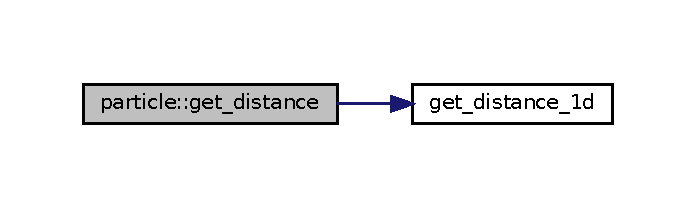
\includegraphics[width=334pt]{structparticle_ab28d2ff9718bfa0fb801275d90f36a9d_cgraph}
\end{center}
\end{figure}
\mbox{\Hypertarget{structparticle_a74457d580da5637e77c1d72ba7a31bb5}\label{structparticle_a74457d580da5637e77c1d72ba7a31bb5}} 
\index{particle@{particle}!get\+\_\+info@{get\+\_\+info}}
\index{get\+\_\+info@{get\+\_\+info}!particle@{particle}}
\subsubsection{\texorpdfstring{get\+\_\+info()}{get\_info()}}
{\footnotesize\ttfamily std\+::string particle\+::get\+\_\+info (\begin{DoxyParamCaption}\item[{void}]{ }\end{DoxyParamCaption})}

Return info of particle \begin{DoxyReturn}{Returns}

\end{DoxyReturn}


Definition at line 335 of file Class\+Siec.\+cpp.



References nr, pos, t, and vel.

\mbox{\Hypertarget{structparticle_a8075edc35cef018e8d5fabcce3bc099e}\label{structparticle_a8075edc35cef018e8d5fabcce3bc099e}} 
\index{particle@{particle}!get\+\_\+time\+\_\+to\+\_\+collision@{get\+\_\+time\+\_\+to\+\_\+collision}}
\index{get\+\_\+time\+\_\+to\+\_\+collision@{get\+\_\+time\+\_\+to\+\_\+collision}!particle@{particle}}
\subsubsection{\texorpdfstring{get\+\_\+time\+\_\+to\+\_\+collision()}{get\_time\_to\_collision()}}
{\footnotesize\ttfamily double particle\+::get\+\_\+time\+\_\+to\+\_\+collision (\begin{DoxyParamCaption}\item[{\mbox{\hyperlink{structparticle}{particle}} $\ast$}]{to\+\_\+particle,  }\item[{double}]{box\+\_\+x = {\ttfamily 0.0},  }\item[{double}]{box\+\_\+y = {\ttfamily 0.0} }\end{DoxyParamCaption})}

Calculate time to colision with particle 
\begin{DoxyParams}{Parameters}
{\em to\+\_\+particle} & \\
\hline
{\em box\+\_\+x} & \\
\hline
{\em box\+\_\+y} & \\
\hline
\end{DoxyParams}
\begin{DoxyReturn}{Returns}

\end{DoxyReturn}


Definition at line 301 of file Class\+Siec.\+cpp.



References get\+\_\+distance(), get\+\_\+distance\+\_\+1d(), pos, r, and vel.

Here is the call graph for this function\+:\nopagebreak
\begin{figure}[H]
\begin{center}
\leavevmode
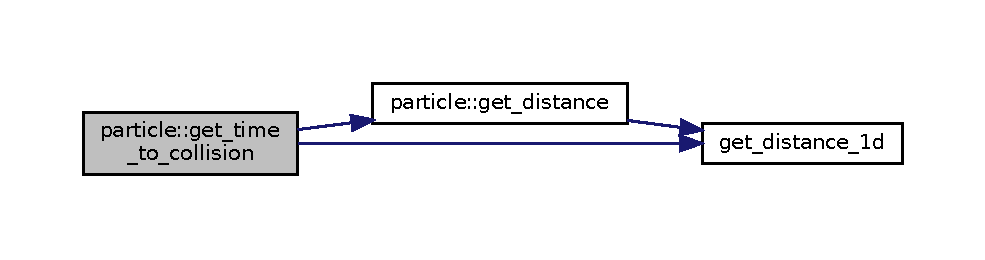
\includegraphics[width=350pt]{structparticle_a8075edc35cef018e8d5fabcce3bc099e_cgraph}
\end{center}
\end{figure}
\mbox{\Hypertarget{structparticle_a8ca7119317b6176296ba0e4a0734ee33}\label{structparticle_a8ca7119317b6176296ba0e4a0734ee33}} 
\index{particle@{particle}!get\+\_\+velocity@{get\+\_\+velocity}}
\index{get\+\_\+velocity@{get\+\_\+velocity}!particle@{particle}}
\subsubsection{\texorpdfstring{get\+\_\+velocity()}{get\_velocity()}}
{\footnotesize\ttfamily double particle\+::get\+\_\+velocity (\begin{DoxyParamCaption}\item[{void}]{ }\end{DoxyParamCaption})}

Calculate velocity \begin{DoxyReturn}{Returns}

\end{DoxyReturn}


Definition at line 289 of file Class\+Siec.\+cpp.



References vel.



Referenced by Class\+Siec\+::step\+\_\+all().

\mbox{\Hypertarget{structparticle_af0c523c22c7b51a1a932f5f3f30b24a3}\label{structparticle_af0c523c22c7b51a1a932f5f3f30b24a3}} 
\index{particle@{particle}!set\+\_\+mass@{set\+\_\+mass}}
\index{set\+\_\+mass@{set\+\_\+mass}!particle@{particle}}
\subsubsection{\texorpdfstring{set\+\_\+mass()}{set\_mass()}}
{\footnotesize\ttfamily int particle\+::set\+\_\+mass (\begin{DoxyParamCaption}\item[{double}]{m }\end{DoxyParamCaption})}

Set mass of particle 
\begin{DoxyParams}{Parameters}
{\em m} & \\
\hline
\end{DoxyParams}
\begin{DoxyReturn}{Returns}

\end{DoxyReturn}


Definition at line 134 of file Class\+Siec.\+cpp.



References m, and OK.

\mbox{\Hypertarget{structparticle_a842a75343ebbcdcaf53e95f0f1286d9a}\label{structparticle_a842a75343ebbcdcaf53e95f0f1286d9a}} 
\index{particle@{particle}!set\+\_\+max\+Velocity@{set\+\_\+max\+Velocity}}
\index{set\+\_\+max\+Velocity@{set\+\_\+max\+Velocity}!particle@{particle}}
\subsubsection{\texorpdfstring{set\+\_\+max\+Velocity()}{set\_maxVelocity()}}
{\footnotesize\ttfamily int particle\+::set\+\_\+max\+Velocity (\begin{DoxyParamCaption}\item[{double}]{max\+Velocity }\end{DoxyParamCaption})}

Set max velocity of particle 
\begin{DoxyParams}{Parameters}
{\em max\+Velocity} & \\
\hline
\end{DoxyParams}
\begin{DoxyRefDesc}{Bug}
\item[\mbox{\hyperlink{bug__bug000001}{Bug}}]probably not useful \end{DoxyRefDesc}
\begin{DoxyReturn}{Returns}

\end{DoxyReturn}


Definition at line 184 of file Class\+Siec.\+cpp.



References max\+Velocity, and OK.

\mbox{\Hypertarget{structparticle_a1088eb89ce4d29bc645160b91ba328c3}\label{structparticle_a1088eb89ce4d29bc645160b91ba328c3}} 
\index{particle@{particle}!set\+\_\+pos@{set\+\_\+pos}}
\index{set\+\_\+pos@{set\+\_\+pos}!particle@{particle}}
\subsubsection{\texorpdfstring{set\+\_\+pos()}{set\_pos()}}
{\footnotesize\ttfamily int particle\+::set\+\_\+pos (\begin{DoxyParamCaption}\item[{double}]{x,  }\item[{double}]{y }\end{DoxyParamCaption})}

Set position of particle 
\begin{DoxyParams}{Parameters}
{\em x} & \\
\hline
{\em y} & \\
\hline
\end{DoxyParams}
\begin{DoxyReturn}{Returns}

\end{DoxyReturn}


Definition at line 157 of file Class\+Siec.\+cpp.



References OK, and pos.

\mbox{\Hypertarget{structparticle_ad45d7067a63de0b6c6ce07723a8e7be2}\label{structparticle_ad45d7067a63de0b6c6ce07723a8e7be2}} 
\index{particle@{particle}!set\+\_\+r@{set\+\_\+r}}
\index{set\+\_\+r@{set\+\_\+r}!particle@{particle}}
\subsubsection{\texorpdfstring{set\+\_\+r()}{set\_r()}}
{\footnotesize\ttfamily int particle\+::set\+\_\+r (\begin{DoxyParamCaption}\item[{double}]{r }\end{DoxyParamCaption})}

Set radius of particle 
\begin{DoxyParams}{Parameters}
{\em r} & \\
\hline
\end{DoxyParams}
\begin{DoxyReturn}{Returns}

\end{DoxyReturn}


Definition at line 145 of file Class\+Siec.\+cpp.



References OK, and r.

\mbox{\Hypertarget{structparticle_aafcf36063e5b6b0719b7ee8377f3c880}\label{structparticle_aafcf36063e5b6b0719b7ee8377f3c880}} 
\index{particle@{particle}!set\+\_\+vel@{set\+\_\+vel}}
\index{set\+\_\+vel@{set\+\_\+vel}!particle@{particle}}
\subsubsection{\texorpdfstring{set\+\_\+vel()}{set\_vel()}}
{\footnotesize\ttfamily int particle\+::set\+\_\+vel (\begin{DoxyParamCaption}\item[{double}]{vx,  }\item[{double}]{vy }\end{DoxyParamCaption})}

Set velocity of particle 
\begin{DoxyParams}{Parameters}
{\em vx} & \\
\hline
{\em vy} & \\
\hline
\end{DoxyParams}
\begin{DoxyReturn}{Returns}

\end{DoxyReturn}


Definition at line 170 of file Class\+Siec.\+cpp.



References OK, and vel.

\mbox{\Hypertarget{structparticle_a4f06bd4316643ca9ba721a4f768763a6}\label{structparticle_a4f06bd4316643ca9ba721a4f768763a6}} 
\index{particle@{particle}!step@{step}}
\index{step@{step}!particle@{particle}}
\subsubsection{\texorpdfstring{step()}{step()}}
{\footnotesize\ttfamily int particle\+::step (\begin{DoxyParamCaption}\item[{double}]{dt = {\ttfamily 1.0} }\end{DoxyParamCaption})}

Set step dt 
\begin{DoxyParams}{Parameters}
{\em dt} & \\
\hline
\end{DoxyParams}
\begin{DoxyRefDesc}{Bug}
\item[\mbox{\hyperlink{bug__bug000002}{Bug}}]not useful \end{DoxyRefDesc}
\begin{DoxyReturn}{Returns}

\end{DoxyReturn}


Definition at line 196 of file Class\+Siec.\+cpp.



References OK, pos, t, and vel.



\subsection{Member Data Documentation}
\mbox{\Hypertarget{structparticle_a7ea0e8707e7e91c3f298c5881bce4581}\label{structparticle_a7ea0e8707e7e91c3f298c5881bce4581}} 
\index{particle@{particle}!color@{color}}
\index{color@{color}!particle@{particle}}
\subsubsection{\texorpdfstring{color}{color}}
{\footnotesize\ttfamily A\+L\+L\+E\+G\+R\+O\+\_\+\+C\+O\+L\+OR particle\+::color}



Definition at line 50 of file Class\+Siec.\+h.



Referenced by draw\+\_\+all(), particle(), Class\+Siec\+::step\+\_\+all(), and zderzenie().

\mbox{\Hypertarget{structparticle_a4cb4f184e6cd2b5dc0dc555d14f265dd}\label{structparticle_a4cb4f184e6cd2b5dc0dc555d14f265dd}} 
\index{particle@{particle}!m@{m}}
\index{m@{m}!particle@{particle}}
\subsubsection{\texorpdfstring{m}{m}}
{\footnotesize\ttfamily double particle\+::m}



Definition at line 46 of file Class\+Siec.\+h.



Referenced by particle(), particle\+\_\+zero\+\_\+time\+::particle\+\_\+zero\+\_\+time(), set\+\_\+mass(), and zderzenie().

\mbox{\Hypertarget{structparticle_a2ea1a35ec678df5cc776dfd6bd377fad}\label{structparticle_a2ea1a35ec678df5cc776dfd6bd377fad}} 
\index{particle@{particle}!max\+Velocity@{max\+Velocity}}
\index{max\+Velocity@{max\+Velocity}!particle@{particle}}
\subsubsection{\texorpdfstring{max\+Velocity}{maxVelocity}}
{\footnotesize\ttfamily double particle\+::max\+Velocity}



Definition at line 44 of file Class\+Siec.\+h.



Referenced by particle(), particle\+\_\+zero\+\_\+time\+::particle\+\_\+zero\+\_\+time(), and set\+\_\+max\+Velocity().

\mbox{\Hypertarget{structparticle_a055d478842e85c5f730fc75f16254852}\label{structparticle_a055d478842e85c5f730fc75f16254852}} 
\index{particle@{particle}!nr@{nr}}
\index{nr@{nr}!particle@{particle}}
\subsubsection{\texorpdfstring{nr}{nr}}
{\footnotesize\ttfamily uint64\+\_\+t particle\+::nr}



Definition at line 49 of file Class\+Siec.\+h.



Referenced by get\+\_\+info(), particle(), and particle\+\_\+zero\+\_\+time\+::particle\+\_\+zero\+\_\+time().

\mbox{\Hypertarget{structparticle_a9ba2ff9e556c82ec96f56ce659c1ad50}\label{structparticle_a9ba2ff9e556c82ec96f56ce659c1ad50}} 
\index{particle@{particle}!pos@{pos}}
\index{pos@{pos}!particle@{particle}}
\subsubsection{\texorpdfstring{pos}{pos}}
{\footnotesize\ttfamily double particle\+::pos\mbox{[}2\mbox{]}}



Definition at line 42 of file Class\+Siec.\+h.



Referenced by draw\+\_\+all(), get\+\_\+distance(), get\+\_\+distance\+\_\+2d(), get\+\_\+info(), get\+\_\+time\+\_\+to\+\_\+collision(), particle(), particle\+\_\+zero\+\_\+time\+::particle\+\_\+zero\+\_\+time(), set\+\_\+pos(), step(), Class\+Siec\+::step\+\_\+all(), th\+\_\+to\+\_\+box(), and zderzenie().

\mbox{\Hypertarget{structparticle_a9ba64d6fa0d4bda34688d54a05341b77}\label{structparticle_a9ba64d6fa0d4bda34688d54a05341b77}} 
\index{particle@{particle}!r@{r}}
\index{r@{r}!particle@{particle}}
\subsubsection{\texorpdfstring{r}{r}}
{\footnotesize\ttfamily double particle\+::r}



Definition at line 45 of file Class\+Siec.\+h.



Referenced by draw\+\_\+all(), get\+\_\+time\+\_\+to\+\_\+collision(), particle(), particle\+\_\+zero\+\_\+time\+::particle\+\_\+zero\+\_\+time(), and set\+\_\+r().

\mbox{\Hypertarget{structparticle_a5225483b35b28edcf29be553a367a952}\label{structparticle_a5225483b35b28edcf29be553a367a952}} 
\index{particle@{particle}!t@{t}}
\index{t@{t}!particle@{particle}}
\subsubsection{\texorpdfstring{t}{t}}
{\footnotesize\ttfamily double particle\+::t}



Definition at line 47 of file Class\+Siec.\+h.



Referenced by get\+\_\+info(), particle(), step(), and Class\+Siec\+::step\+\_\+all().

\mbox{\Hypertarget{structparticle_a5ab99949ec29f5623413672b923ffa25}\label{structparticle_a5ab99949ec29f5623413672b923ffa25}} 
\index{particle@{particle}!tlc@{tlc}}
\index{tlc@{tlc}!particle@{particle}}
\subsubsection{\texorpdfstring{tlc}{tlc}}
{\footnotesize\ttfamily double particle\+::tlc}



Definition at line 48 of file Class\+Siec.\+h.



Referenced by particle(), and zderzenie().

\mbox{\Hypertarget{structparticle_abd12470a54dcbf5694c6adeb8c06ef8b}\label{structparticle_abd12470a54dcbf5694c6adeb8c06ef8b}} 
\index{particle@{particle}!vel@{vel}}
\index{vel@{vel}!particle@{particle}}
\subsubsection{\texorpdfstring{vel}{vel}}
{\footnotesize\ttfamily double particle\+::vel\mbox{[}2\mbox{]}}



Definition at line 43 of file Class\+Siec.\+h.



Referenced by draw\+\_\+all(), get\+\_\+info(), get\+\_\+time\+\_\+to\+\_\+collision(), get\+\_\+velocity(), particle(), particle\+\_\+zero\+\_\+time\+::particle\+\_\+zero\+\_\+time(), set\+\_\+vel(), step(), Class\+Siec\+::step\+\_\+all(), and zderzenie().



The documentation for this struct was generated from the following files\+:\begin{DoxyCompactItemize}
\item 
\mbox{\hyperlink{ClassSiec_8h}{Class\+Siec.\+h}}\item 
\mbox{\hyperlink{ClassSiec_8cpp}{Class\+Siec.\+cpp}}\end{DoxyCompactItemize}

\hypertarget{structparticle__zero__time}{}\section{particle\+\_\+zero\+\_\+time Struct Reference}
\label{structparticle__zero__time}\index{particle\+\_\+zero\+\_\+time@{particle\+\_\+zero\+\_\+time}}


{\ttfamily \#include $<$Class\+Siec.\+h$>$}



Collaboration diagram for particle\+\_\+zero\+\_\+time\+:\nopagebreak
\begin{figure}[H]
\begin{center}
\leavevmode
\includegraphics[width=206pt]{structparticle__zero__time__coll__graph}
\end{center}
\end{figure}
\subsection*{Public Member Functions}
\begin{DoxyCompactItemize}
\item 
\mbox{\hyperlink{structparticle__zero__time_ac3abaccc3579eddbe304718deac0bcd0}{particle\+\_\+zero\+\_\+time}} (\mbox{\hyperlink{structparticle}{particle}} $\ast$\mbox{\hyperlink{structparticle}{particle}})
\end{DoxyCompactItemize}
\subsection*{Public Attributes}
\begin{DoxyCompactItemize}
\item 
uint64\+\_\+t \mbox{\hyperlink{structparticle__zero__time_a866e480ab047b43e3654d6843aa44276}{nr}}
\item 
double \mbox{\hyperlink{structparticle__zero__time_a6101461222bc79283b8c8a59cb6e7dee}{pos}} \mbox{[}2\mbox{]}
\item 
double \mbox{\hyperlink{structparticle__zero__time_a02135214c123f6cbc5ca706cdf47c890}{vel}} \mbox{[}2\mbox{]}
\item 
double \mbox{\hyperlink{structparticle__zero__time_a1162e81c9a3fca1545c7ed2b7a1a6140}{max\+Velocity}}
\item 
double \mbox{\hyperlink{structparticle__zero__time_a06f14406f824aaf0c0cd61054876fd56}{r}}
\item 
double \mbox{\hyperlink{structparticle__zero__time_ae75f971e47e3bd12789383dd352a2fa6}{m}}
\item 
double \mbox{\hyperlink{structparticle__zero__time_a09c3ed1201f81f88c5719da195c3c7d1}{velxy}}
\end{DoxyCompactItemize}


\subsection{Detailed Description}


Definition at line 84 of file Class\+Siec.\+h.



\subsection{Constructor \& Destructor Documentation}
\mbox{\Hypertarget{structparticle__zero__time_ac3abaccc3579eddbe304718deac0bcd0}\label{structparticle__zero__time_ac3abaccc3579eddbe304718deac0bcd0}} 
\index{particle\+\_\+zero\+\_\+time@{particle\+\_\+zero\+\_\+time}!particle\+\_\+zero\+\_\+time@{particle\+\_\+zero\+\_\+time}}
\index{particle\+\_\+zero\+\_\+time@{particle\+\_\+zero\+\_\+time}!particle\+\_\+zero\+\_\+time@{particle\+\_\+zero\+\_\+time}}
\subsubsection{\texorpdfstring{particle\+\_\+zero\+\_\+time()}{particle\_zero\_time()}}
{\footnotesize\ttfamily particle\+\_\+zero\+\_\+time\+::particle\+\_\+zero\+\_\+time (\begin{DoxyParamCaption}\item[{\mbox{\hyperlink{structparticle}{particle}} $\ast$}]{particle }\end{DoxyParamCaption})}

Generate zero time particle 
\begin{DoxyParams}{Parameters}
{\em particle} & \\
\hline
\end{DoxyParams}


Definition at line 208 of file Class\+Siec.\+cpp.



References particle\+::m, m, particle\+::max\+Velocity, max\+Velocity, particle\+::nr, nr, particle\+::pos, pos, particle\+::r, r, particle\+::vel, vel, and velxy.



\subsection{Member Data Documentation}
\mbox{\Hypertarget{structparticle__zero__time_ae75f971e47e3bd12789383dd352a2fa6}\label{structparticle__zero__time_ae75f971e47e3bd12789383dd352a2fa6}} 
\index{particle\+\_\+zero\+\_\+time@{particle\+\_\+zero\+\_\+time}!m@{m}}
\index{m@{m}!particle\+\_\+zero\+\_\+time@{particle\+\_\+zero\+\_\+time}}
\subsubsection{\texorpdfstring{m}{m}}
{\footnotesize\ttfamily double particle\+\_\+zero\+\_\+time\+::m}



Definition at line 92 of file Class\+Siec.\+h.



Referenced by particle\+\_\+zero\+\_\+time().

\mbox{\Hypertarget{structparticle__zero__time_a1162e81c9a3fca1545c7ed2b7a1a6140}\label{structparticle__zero__time_a1162e81c9a3fca1545c7ed2b7a1a6140}} 
\index{particle\+\_\+zero\+\_\+time@{particle\+\_\+zero\+\_\+time}!max\+Velocity@{max\+Velocity}}
\index{max\+Velocity@{max\+Velocity}!particle\+\_\+zero\+\_\+time@{particle\+\_\+zero\+\_\+time}}
\subsubsection{\texorpdfstring{max\+Velocity}{maxVelocity}}
{\footnotesize\ttfamily double particle\+\_\+zero\+\_\+time\+::max\+Velocity}



Definition at line 90 of file Class\+Siec.\+h.



Referenced by particle\+\_\+zero\+\_\+time().

\mbox{\Hypertarget{structparticle__zero__time_a866e480ab047b43e3654d6843aa44276}\label{structparticle__zero__time_a866e480ab047b43e3654d6843aa44276}} 
\index{particle\+\_\+zero\+\_\+time@{particle\+\_\+zero\+\_\+time}!nr@{nr}}
\index{nr@{nr}!particle\+\_\+zero\+\_\+time@{particle\+\_\+zero\+\_\+time}}
\subsubsection{\texorpdfstring{nr}{nr}}
{\footnotesize\ttfamily uint64\+\_\+t particle\+\_\+zero\+\_\+time\+::nr}



Definition at line 87 of file Class\+Siec.\+h.



Referenced by particle\+\_\+zero\+\_\+time().

\mbox{\Hypertarget{structparticle__zero__time_a6101461222bc79283b8c8a59cb6e7dee}\label{structparticle__zero__time_a6101461222bc79283b8c8a59cb6e7dee}} 
\index{particle\+\_\+zero\+\_\+time@{particle\+\_\+zero\+\_\+time}!pos@{pos}}
\index{pos@{pos}!particle\+\_\+zero\+\_\+time@{particle\+\_\+zero\+\_\+time}}
\subsubsection{\texorpdfstring{pos}{pos}}
{\footnotesize\ttfamily double particle\+\_\+zero\+\_\+time\+::pos\mbox{[}2\mbox{]}}



Definition at line 88 of file Class\+Siec.\+h.



Referenced by particle\+\_\+zero\+\_\+time().

\mbox{\Hypertarget{structparticle__zero__time_a06f14406f824aaf0c0cd61054876fd56}\label{structparticle__zero__time_a06f14406f824aaf0c0cd61054876fd56}} 
\index{particle\+\_\+zero\+\_\+time@{particle\+\_\+zero\+\_\+time}!r@{r}}
\index{r@{r}!particle\+\_\+zero\+\_\+time@{particle\+\_\+zero\+\_\+time}}
\subsubsection{\texorpdfstring{r}{r}}
{\footnotesize\ttfamily double particle\+\_\+zero\+\_\+time\+::r}



Definition at line 91 of file Class\+Siec.\+h.



Referenced by particle\+\_\+zero\+\_\+time().

\mbox{\Hypertarget{structparticle__zero__time_a02135214c123f6cbc5ca706cdf47c890}\label{structparticle__zero__time_a02135214c123f6cbc5ca706cdf47c890}} 
\index{particle\+\_\+zero\+\_\+time@{particle\+\_\+zero\+\_\+time}!vel@{vel}}
\index{vel@{vel}!particle\+\_\+zero\+\_\+time@{particle\+\_\+zero\+\_\+time}}
\subsubsection{\texorpdfstring{vel}{vel}}
{\footnotesize\ttfamily double particle\+\_\+zero\+\_\+time\+::vel\mbox{[}2\mbox{]}}



Definition at line 89 of file Class\+Siec.\+h.



Referenced by particle\+\_\+zero\+\_\+time().

\mbox{\Hypertarget{structparticle__zero__time_a09c3ed1201f81f88c5719da195c3c7d1}\label{structparticle__zero__time_a09c3ed1201f81f88c5719da195c3c7d1}} 
\index{particle\+\_\+zero\+\_\+time@{particle\+\_\+zero\+\_\+time}!velxy@{velxy}}
\index{velxy@{velxy}!particle\+\_\+zero\+\_\+time@{particle\+\_\+zero\+\_\+time}}
\subsubsection{\texorpdfstring{velxy}{velxy}}
{\footnotesize\ttfamily double particle\+\_\+zero\+\_\+time\+::velxy}



Definition at line 93 of file Class\+Siec.\+h.



Referenced by particle\+\_\+zero\+\_\+time().



The documentation for this struct was generated from the following files\+:\begin{DoxyCompactItemize}
\item 
\mbox{\hyperlink{ClassSiec_8h}{Class\+Siec.\+h}}\item 
\mbox{\hyperlink{ClassSiec_8cpp}{Class\+Siec.\+cpp}}\end{DoxyCompactItemize}

\hypertarget{structs__pair}{}\section{s\+\_\+pair Struct Reference}
\label{structs__pair}\index{s\+\_\+pair@{s\+\_\+pair}}


{\ttfamily \#include $<$Class\+Siec.\+h$>$}



Collaboration diagram for s\+\_\+pair\+:\nopagebreak
\begin{figure}[H]
\begin{center}
\leavevmode
\includegraphics[width=145pt]{structs__pair__coll__graph}
\end{center}
\end{figure}
\subsection*{Public Member Functions}
\begin{DoxyCompactItemize}
\item 
\mbox{\hyperlink{structs__pair_aee9b5834540a69b1f920276f9f069715}{s\+\_\+pair}} (uint64\+\_\+t \mbox{\hyperlink{structs__pair_aa255b01b871f0a9d8236717b13c4c167}{a}}, uint64\+\_\+t \mbox{\hyperlink{structs__pair_a4b452c86a4f4005ef2781e0324a50dda}{b}}, double \mbox{\hyperlink{structs__pair_a6da5de6a04996b5b5c26be868da76900}{dt}})
\end{DoxyCompactItemize}
\subsection*{Public Attributes}
\begin{DoxyCompactItemize}
\item 
uint64\+\_\+t \mbox{\hyperlink{structs__pair_aa255b01b871f0a9d8236717b13c4c167}{a}}
\item 
uint64\+\_\+t \mbox{\hyperlink{structs__pair_a4b452c86a4f4005ef2781e0324a50dda}{b}}
\item 
double \mbox{\hyperlink{structs__pair_a6da5de6a04996b5b5c26be868da76900}{dt}}
\end{DoxyCompactItemize}


\subsection{Detailed Description}


Definition at line 76 of file Class\+Siec.\+h.



\subsection{Constructor \& Destructor Documentation}
\mbox{\Hypertarget{structs__pair_aee9b5834540a69b1f920276f9f069715}\label{structs__pair_aee9b5834540a69b1f920276f9f069715}} 
\index{s\+\_\+pair@{s\+\_\+pair}!s\+\_\+pair@{s\+\_\+pair}}
\index{s\+\_\+pair@{s\+\_\+pair}!s\+\_\+pair@{s\+\_\+pair}}
\subsubsection{\texorpdfstring{s\+\_\+pair()}{s\_pair()}}
{\footnotesize\ttfamily s\+\_\+pair\+::s\+\_\+pair (\begin{DoxyParamCaption}\item[{uint64\+\_\+t}]{a,  }\item[{uint64\+\_\+t}]{b,  }\item[{double}]{dt }\end{DoxyParamCaption})}

Constructor for pair of particles 
\begin{DoxyParams}{Parameters}
{\em a} & \\
\hline
{\em b} & \\
\hline
{\em dt} & \\
\hline
\end{DoxyParams}


Definition at line 850 of file Class\+Siec.\+cpp.



References a, b, and dt.



\subsection{Member Data Documentation}
\mbox{\Hypertarget{structs__pair_aa255b01b871f0a9d8236717b13c4c167}\label{structs__pair_aa255b01b871f0a9d8236717b13c4c167}} 
\index{s\+\_\+pair@{s\+\_\+pair}!a@{a}}
\index{a@{a}!s\+\_\+pair@{s\+\_\+pair}}
\subsubsection{\texorpdfstring{a}{a}}
{\footnotesize\ttfamily uint64\+\_\+t s\+\_\+pair\+::a}



Definition at line 79 of file Class\+Siec.\+h.



Referenced by s\+\_\+pair().

\mbox{\Hypertarget{structs__pair_a4b452c86a4f4005ef2781e0324a50dda}\label{structs__pair_a4b452c86a4f4005ef2781e0324a50dda}} 
\index{s\+\_\+pair@{s\+\_\+pair}!b@{b}}
\index{b@{b}!s\+\_\+pair@{s\+\_\+pair}}
\subsubsection{\texorpdfstring{b}{b}}
{\footnotesize\ttfamily uint64\+\_\+t s\+\_\+pair\+::b}



Definition at line 80 of file Class\+Siec.\+h.



Referenced by s\+\_\+pair().

\mbox{\Hypertarget{structs__pair_a6da5de6a04996b5b5c26be868da76900}\label{structs__pair_a6da5de6a04996b5b5c26be868da76900}} 
\index{s\+\_\+pair@{s\+\_\+pair}!dt@{dt}}
\index{dt@{dt}!s\+\_\+pair@{s\+\_\+pair}}
\subsubsection{\texorpdfstring{dt}{dt}}
{\footnotesize\ttfamily double s\+\_\+pair\+::dt}



Definition at line 81 of file Class\+Siec.\+h.



Referenced by s\+\_\+pair().



The documentation for this struct was generated from the following files\+:\begin{DoxyCompactItemize}
\item 
\mbox{\hyperlink{ClassSiec_8h}{Class\+Siec.\+h}}\item 
\mbox{\hyperlink{ClassSiec_8cpp}{Class\+Siec.\+cpp}}\end{DoxyCompactItemize}

\chapter{File Documentation}
\hypertarget{ClassSiec_8cpp}{}\section{Class\+Siec.\+cpp File Reference}
\label{ClassSiec_8cpp}\index{Class\+Siec.\+cpp@{Class\+Siec.\+cpp}}
{\ttfamily \#include \char`\"{}Class\+Siec.\+h\char`\"{}}\newline
Include dependency graph for Class\+Siec.\+cpp\+:\nopagebreak
\begin{figure}[H]
\begin{center}
\leavevmode
\includegraphics[width=350pt]{ClassSiec_8cpp__incl}
\end{center}
\end{figure}
\subsection*{Functions}
\begin{DoxyCompactItemize}
\item 
{\footnotesize template$<$class T $>$ }\\T \mbox{\hyperlink{ClassSiec_8cpp_aa11e584dd125456775429c3b9a75b242}{find\+\_\+max}} (T $\ast$data, uint64\+\_\+t size)
\item 
{\footnotesize template$<$class T $>$ }\\T \mbox{\hyperlink{ClassSiec_8cpp_a203a64f321b303a7af6ce1072aa442ce}{find\+\_\+min}} (T $\ast$data, uint64\+\_\+t size)
\item 
{\footnotesize template$<$class T $>$ }\\T \mbox{\hyperlink{ClassSiec_8cpp_ac51862e2cdf2f570d5c330d6ace2ff85}{find\+\_\+max}} (vector$<$ T $>$ \&data)
\item 
{\footnotesize template$<$class T $>$ }\\T \mbox{\hyperlink{ClassSiec_8cpp_a0a23711d23c9a45599f6b45c55d18359}{find\+\_\+min}} (vector$<$ T $>$ \&data)
\item 
{\footnotesize template$<$class T $>$ }\\T \mbox{\hyperlink{ClassSiec_8cpp_aca9faddeba784ab395dfac83f93fd341}{find\+\_\+delta}} (vector$<$ T $>$ \&data)
\item 
{\footnotesize template$<$class T $>$ }\\T \mbox{\hyperlink{ClassSiec_8cpp_a080bc004de0a84b7dce1cc40943d2356}{find\+\_\+sum}} (vector$<$ T $>$ \&data)
\item 
{\footnotesize template$<$class T $>$ }\\T \mbox{\hyperlink{ClassSiec_8cpp_a98d2fa9d1a1f6487fbdc786d6b6bda9a}{find\+\_\+average}} (vector$<$ T $>$ \&data)
\item 
{\footnotesize template$<$typename Type $>$ }\\void \mbox{\hyperlink{ClassSiec_8cpp_a5e38df1fbf45b8b1619cfaeeb056d533}{remove\+\_\+duplicate}} (std\+::vector$<$ Type $>$ vec)
\item 
{\footnotesize template$<$typename Type $>$ }\\void \mbox{\hyperlink{ClassSiec_8cpp_a9fb993c96006ec4443e6d0d38bff9247}{remove\+\_\+duplicate2}} (std\+::vector$<$ Type $>$ vec)
\item 
int \mbox{\hyperlink{ClassSiec_8cpp_aebe3c045134bed926d50d2b6e36e39d1}{find\+\_\+is\+\_\+in\+\_\+range}} (double value, double centrum, double delta)
\item 
int \mbox{\hyperlink{ClassSiec_8cpp_a0af26329b21bf468404bc298ef514fcd}{find\+\_\+is\+\_\+in\+\_\+range}} (double value, double centrum, double left, double right)
\item 
double \mbox{\hyperlink{ClassSiec_8cpp_aa4200d584f59d89ab0cce9d85f99a564}{get\+\_\+distance\+\_\+1d}} (double x0, double x1, double box\+\_\+x)
\item 
double \mbox{\hyperlink{ClassSiec_8cpp_a71b54469f61e2266d054d489957cf8cf}{get\+\_\+distance\+\_\+2d}} (\mbox{\hyperlink{structparticle}{particle}} $\ast$p0, \mbox{\hyperlink{structparticle}{particle}} $\ast$p1, double box\+\_\+x, double box\+\_\+y)
\item 
double \mbox{\hyperlink{ClassSiec_8cpp_ad2771c2f42d6323693918169e3e50e1d}{get\+\_\+distance\+\_\+2d}} (double x0, double y0, double x1, double y1, double box\+\_\+x, double box\+\_\+y)
\item 
void \mbox{\hyperlink{ClassSiec_8cpp_aef01d17806faa9f0650648d16bfdc027}{th\+\_\+to\+\_\+box}} (\mbox{\hyperlink{structparticle}{particle}} $\ast$\mbox{\hyperlink{structparticle}{particle}}, double box\+\_\+x=0.\+0, double box\+\_\+y=0.\+0)
\item 
int \mbox{\hyperlink{ClassSiec_8cpp_a45867c7613dff6802723ff7e0017269b}{zderzenie}} (\mbox{\hyperlink{structparticle}{particle}} $\ast$cz0, \mbox{\hyperlink{structparticle}{particle}} $\ast$cz1, double box\+\_\+x, double box\+\_\+y)
\item 
int \mbox{\hyperlink{ClassSiec_8cpp_ac09c4f66afc9dffbec912d9b227af15d}{save\+\_\+to\+\_\+file}} (std\+::string filename, std\+::string data)
\item 
void \mbox{\hyperlink{ClassSiec_8cpp_a1dceb3757345c2076aaad796810fc100}{thread\+\_\+\+R\+DF}} (\mbox{\hyperlink{classClassSiec}{Class\+Siec}} $\ast$siec, uint64\+\_\+t c1, double prec)
\end{DoxyCompactItemize}


\subsection{Function Documentation}
\mbox{\Hypertarget{ClassSiec_8cpp_a98d2fa9d1a1f6487fbdc786d6b6bda9a}\label{ClassSiec_8cpp_a98d2fa9d1a1f6487fbdc786d6b6bda9a}} 
\index{Class\+Siec.\+cpp@{Class\+Siec.\+cpp}!find\+\_\+average@{find\+\_\+average}}
\index{find\+\_\+average@{find\+\_\+average}!Class\+Siec.\+cpp@{Class\+Siec.\+cpp}}
\subsubsection{\texorpdfstring{find\+\_\+average()}{find\_average()}}
{\footnotesize\ttfamily template$<$class T $>$ \\
T find\+\_\+average (\begin{DoxyParamCaption}\item[{vector$<$ T $>$ \&}]{data }\end{DoxyParamCaption})}



Definition at line 79 of file Class\+Siec.\+cpp.

\mbox{\Hypertarget{ClassSiec_8cpp_aca9faddeba784ab395dfac83f93fd341}\label{ClassSiec_8cpp_aca9faddeba784ab395dfac83f93fd341}} 
\index{Class\+Siec.\+cpp@{Class\+Siec.\+cpp}!find\+\_\+delta@{find\+\_\+delta}}
\index{find\+\_\+delta@{find\+\_\+delta}!Class\+Siec.\+cpp@{Class\+Siec.\+cpp}}
\subsubsection{\texorpdfstring{find\+\_\+delta()}{find\_delta()}}
{\footnotesize\ttfamily template$<$class T $>$ \\
T find\+\_\+delta (\begin{DoxyParamCaption}\item[{vector$<$ T $>$ \&}]{data }\end{DoxyParamCaption})}



Definition at line 51 of file Class\+Siec.\+cpp.



Referenced by Class\+Siec\+::get\+\_\+diffusitivity\+\_\+delta(), Class\+Siec\+::get\+\_\+diffusitivity\+\_\+delta\+\_\+ratio(), Class\+Siec\+::get\+\_\+\+Velocity\+\_\+\+Autocorrelation\+\_\+\+Function\+\_\+delta(), and Class\+Siec\+::get\+\_\+\+Velocity\+\_\+\+Autocorrelation\+\_\+\+Function\+\_\+delta\+\_\+ratio().

\mbox{\Hypertarget{ClassSiec_8cpp_aebe3c045134bed926d50d2b6e36e39d1}\label{ClassSiec_8cpp_aebe3c045134bed926d50d2b6e36e39d1}} 
\index{Class\+Siec.\+cpp@{Class\+Siec.\+cpp}!find\+\_\+is\+\_\+in\+\_\+range@{find\+\_\+is\+\_\+in\+\_\+range}}
\index{find\+\_\+is\+\_\+in\+\_\+range@{find\+\_\+is\+\_\+in\+\_\+range}!Class\+Siec.\+cpp@{Class\+Siec.\+cpp}}
\subsubsection{\texorpdfstring{find\+\_\+is\+\_\+in\+\_\+range()}{find\_is\_in\_range()}\hspace{0.1cm}{\footnotesize\ttfamily [1/2]}}
{\footnotesize\ttfamily int find\+\_\+is\+\_\+in\+\_\+range (\begin{DoxyParamCaption}\item[{double}]{value,  }\item[{double}]{centrum,  }\item[{double}]{delta }\end{DoxyParamCaption})}



Definition at line 103 of file Class\+Siec.\+cpp.



Referenced by Class\+Siec\+::create\+\_\+hexagonal(), Class\+Siec\+::create\+\_\+honeycomb(), Class\+Siec\+::set\+\_\+momentum\+\_\+to\+\_\+zero(), and thread\+\_\+siec().

\mbox{\Hypertarget{ClassSiec_8cpp_a0af26329b21bf468404bc298ef514fcd}\label{ClassSiec_8cpp_a0af26329b21bf468404bc298ef514fcd}} 
\index{Class\+Siec.\+cpp@{Class\+Siec.\+cpp}!find\+\_\+is\+\_\+in\+\_\+range@{find\+\_\+is\+\_\+in\+\_\+range}}
\index{find\+\_\+is\+\_\+in\+\_\+range@{find\+\_\+is\+\_\+in\+\_\+range}!Class\+Siec.\+cpp@{Class\+Siec.\+cpp}}
\subsubsection{\texorpdfstring{find\+\_\+is\+\_\+in\+\_\+range()}{find\_is\_in\_range()}\hspace{0.1cm}{\footnotesize\ttfamily [2/2]}}
{\footnotesize\ttfamily int find\+\_\+is\+\_\+in\+\_\+range (\begin{DoxyParamCaption}\item[{double}]{value,  }\item[{double}]{centrum,  }\item[{double}]{left,  }\item[{double}]{right }\end{DoxyParamCaption})}



Definition at line 108 of file Class\+Siec.\+cpp.

\mbox{\Hypertarget{ClassSiec_8cpp_aa11e584dd125456775429c3b9a75b242}\label{ClassSiec_8cpp_aa11e584dd125456775429c3b9a75b242}} 
\index{Class\+Siec.\+cpp@{Class\+Siec.\+cpp}!find\+\_\+max@{find\+\_\+max}}
\index{find\+\_\+max@{find\+\_\+max}!Class\+Siec.\+cpp@{Class\+Siec.\+cpp}}
\subsubsection{\texorpdfstring{find\+\_\+max()}{find\_max()}\hspace{0.1cm}{\footnotesize\ttfamily [1/2]}}
{\footnotesize\ttfamily template$<$class T $>$ \\
T find\+\_\+max (\begin{DoxyParamCaption}\item[{T $\ast$}]{data,  }\item[{uint64\+\_\+t}]{size }\end{DoxyParamCaption})}



Definition at line 3 of file Class\+Siec.\+cpp.

\mbox{\Hypertarget{ClassSiec_8cpp_ac51862e2cdf2f570d5c330d6ace2ff85}\label{ClassSiec_8cpp_ac51862e2cdf2f570d5c330d6ace2ff85}} 
\index{Class\+Siec.\+cpp@{Class\+Siec.\+cpp}!find\+\_\+max@{find\+\_\+max}}
\index{find\+\_\+max@{find\+\_\+max}!Class\+Siec.\+cpp@{Class\+Siec.\+cpp}}
\subsubsection{\texorpdfstring{find\+\_\+max()}{find\_max()}\hspace{0.1cm}{\footnotesize\ttfamily [2/2]}}
{\footnotesize\ttfamily template$<$class T $>$ \\
T find\+\_\+max (\begin{DoxyParamCaption}\item[{vector$<$ T $>$ \&}]{data }\end{DoxyParamCaption})}



Definition at line 25 of file Class\+Siec.\+cpp.

\mbox{\Hypertarget{ClassSiec_8cpp_a203a64f321b303a7af6ce1072aa442ce}\label{ClassSiec_8cpp_a203a64f321b303a7af6ce1072aa442ce}} 
\index{Class\+Siec.\+cpp@{Class\+Siec.\+cpp}!find\+\_\+min@{find\+\_\+min}}
\index{find\+\_\+min@{find\+\_\+min}!Class\+Siec.\+cpp@{Class\+Siec.\+cpp}}
\subsubsection{\texorpdfstring{find\+\_\+min()}{find\_min()}\hspace{0.1cm}{\footnotesize\ttfamily [1/2]}}
{\footnotesize\ttfamily template$<$class T $>$ \\
T find\+\_\+min (\begin{DoxyParamCaption}\item[{T $\ast$}]{data,  }\item[{uint64\+\_\+t}]{size }\end{DoxyParamCaption})}



Definition at line 12 of file Class\+Siec.\+cpp.

\mbox{\Hypertarget{ClassSiec_8cpp_a0a23711d23c9a45599f6b45c55d18359}\label{ClassSiec_8cpp_a0a23711d23c9a45599f6b45c55d18359}} 
\index{Class\+Siec.\+cpp@{Class\+Siec.\+cpp}!find\+\_\+min@{find\+\_\+min}}
\index{find\+\_\+min@{find\+\_\+min}!Class\+Siec.\+cpp@{Class\+Siec.\+cpp}}
\subsubsection{\texorpdfstring{find\+\_\+min()}{find\_min()}\hspace{0.1cm}{\footnotesize\ttfamily [2/2]}}
{\footnotesize\ttfamily template$<$class T $>$ \\
T find\+\_\+min (\begin{DoxyParamCaption}\item[{vector$<$ T $>$ \&}]{data }\end{DoxyParamCaption})}



Definition at line 38 of file Class\+Siec.\+cpp.

\mbox{\Hypertarget{ClassSiec_8cpp_a080bc004de0a84b7dce1cc40943d2356}\label{ClassSiec_8cpp_a080bc004de0a84b7dce1cc40943d2356}} 
\index{Class\+Siec.\+cpp@{Class\+Siec.\+cpp}!find\+\_\+sum@{find\+\_\+sum}}
\index{find\+\_\+sum@{find\+\_\+sum}!Class\+Siec.\+cpp@{Class\+Siec.\+cpp}}
\subsubsection{\texorpdfstring{find\+\_\+sum()}{find\_sum()}}
{\footnotesize\ttfamily template$<$class T $>$ \\
T find\+\_\+sum (\begin{DoxyParamCaption}\item[{vector$<$ T $>$ \&}]{data }\end{DoxyParamCaption})}



Definition at line 69 of file Class\+Siec.\+cpp.

\mbox{\Hypertarget{ClassSiec_8cpp_aa4200d584f59d89ab0cce9d85f99a564}\label{ClassSiec_8cpp_aa4200d584f59d89ab0cce9d85f99a564}} 
\index{Class\+Siec.\+cpp@{Class\+Siec.\+cpp}!get\+\_\+distance\+\_\+1d@{get\+\_\+distance\+\_\+1d}}
\index{get\+\_\+distance\+\_\+1d@{get\+\_\+distance\+\_\+1d}!Class\+Siec.\+cpp@{Class\+Siec.\+cpp}}
\subsubsection{\texorpdfstring{get\+\_\+distance\+\_\+1d()}{get\_distance\_1d()}}
{\footnotesize\ttfamily double get\+\_\+distance\+\_\+1d (\begin{DoxyParamCaption}\item[{double}]{x0,  }\item[{double}]{x1,  }\item[{double}]{box\+\_\+x }\end{DoxyParamCaption})}

Calculate the distance in box 
\begin{DoxyParams}{Parameters}
{\em x0} & \\
\hline
{\em x1} & \\
\hline
{\em box\+\_\+x} & \\
\hline
\end{DoxyParams}
\begin{DoxyReturn}{Returns}

\end{DoxyReturn}


Definition at line 228 of file Class\+Siec.\+cpp.



Referenced by particle\+::get\+\_\+distance(), get\+\_\+distance\+\_\+2d(), particle\+::get\+\_\+time\+\_\+to\+\_\+collision(), and zderzenie().

\mbox{\Hypertarget{ClassSiec_8cpp_a71b54469f61e2266d054d489957cf8cf}\label{ClassSiec_8cpp_a71b54469f61e2266d054d489957cf8cf}} 
\index{Class\+Siec.\+cpp@{Class\+Siec.\+cpp}!get\+\_\+distance\+\_\+2d@{get\+\_\+distance\+\_\+2d}}
\index{get\+\_\+distance\+\_\+2d@{get\+\_\+distance\+\_\+2d}!Class\+Siec.\+cpp@{Class\+Siec.\+cpp}}
\subsubsection{\texorpdfstring{get\+\_\+distance\+\_\+2d()}{get\_distance\_2d()}\hspace{0.1cm}{\footnotesize\ttfamily [1/2]}}
{\footnotesize\ttfamily double get\+\_\+distance\+\_\+2d (\begin{DoxyParamCaption}\item[{\mbox{\hyperlink{structparticle}{particle}} $\ast$}]{p0,  }\item[{\mbox{\hyperlink{structparticle}{particle}} $\ast$}]{p1,  }\item[{double}]{box\+\_\+x,  }\item[{double}]{box\+\_\+y }\end{DoxyParamCaption})}

Calculate distance in 2D in box 
\begin{DoxyParams}{Parameters}
{\em p0} & \\
\hline
{\em p1} & \\
\hline
{\em box\+\_\+x} & \\
\hline
{\em box\+\_\+y} & \\
\hline
\end{DoxyParams}
\begin{DoxyReturn}{Returns}

\end{DoxyReturn}


Definition at line 246 of file Class\+Siec.\+cpp.



References get\+\_\+distance\+\_\+1d(), and particle\+::pos.



Referenced by Class\+Siec\+::get\+\_\+number\+\_\+of\+\_\+particles\+\_\+in\+\_\+radius().

Here is the call graph for this function\+:\nopagebreak
\begin{figure}[H]
\begin{center}
\leavevmode
\includegraphics[width=308pt]{ClassSiec_8cpp_a71b54469f61e2266d054d489957cf8cf_cgraph}
\end{center}
\end{figure}
\mbox{\Hypertarget{ClassSiec_8cpp_ad2771c2f42d6323693918169e3e50e1d}\label{ClassSiec_8cpp_ad2771c2f42d6323693918169e3e50e1d}} 
\index{Class\+Siec.\+cpp@{Class\+Siec.\+cpp}!get\+\_\+distance\+\_\+2d@{get\+\_\+distance\+\_\+2d}}
\index{get\+\_\+distance\+\_\+2d@{get\+\_\+distance\+\_\+2d}!Class\+Siec.\+cpp@{Class\+Siec.\+cpp}}
\subsubsection{\texorpdfstring{get\+\_\+distance\+\_\+2d()}{get\_distance\_2d()}\hspace{0.1cm}{\footnotesize\ttfamily [2/2]}}
{\footnotesize\ttfamily double get\+\_\+distance\+\_\+2d (\begin{DoxyParamCaption}\item[{double}]{x0,  }\item[{double}]{y0,  }\item[{double}]{x1,  }\item[{double}]{y1,  }\item[{double}]{box\+\_\+x,  }\item[{double}]{box\+\_\+y }\end{DoxyParamCaption})}

Calculate distance in 2D in box 
\begin{DoxyParams}{Parameters}
{\em x0} & \\
\hline
{\em y0} & \\
\hline
{\em x1} & \\
\hline
{\em y1} & \\
\hline
{\em box\+\_\+x} & \\
\hline
{\em box\+\_\+y} & \\
\hline
\end{DoxyParams}
\begin{DoxyReturn}{Returns}

\end{DoxyReturn}


Definition at line 263 of file Class\+Siec.\+cpp.



References get\+\_\+distance\+\_\+1d().

Here is the call graph for this function\+:\nopagebreak
\begin{figure}[H]
\begin{center}
\leavevmode
\includegraphics[width=308pt]{ClassSiec_8cpp_ad2771c2f42d6323693918169e3e50e1d_cgraph}
\end{center}
\end{figure}
\mbox{\Hypertarget{ClassSiec_8cpp_a5e38df1fbf45b8b1619cfaeeb056d533}\label{ClassSiec_8cpp_a5e38df1fbf45b8b1619cfaeeb056d533}} 
\index{Class\+Siec.\+cpp@{Class\+Siec.\+cpp}!remove\+\_\+duplicate@{remove\+\_\+duplicate}}
\index{remove\+\_\+duplicate@{remove\+\_\+duplicate}!Class\+Siec.\+cpp@{Class\+Siec.\+cpp}}
\subsubsection{\texorpdfstring{remove\+\_\+duplicate()}{remove\_duplicate()}}
{\footnotesize\ttfamily template$<$typename Type $>$ \\
void remove\+\_\+duplicate (\begin{DoxyParamCaption}\item[{std\+::vector$<$ Type $>$}]{vec }\end{DoxyParamCaption})}



Definition at line 90 of file Class\+Siec.\+cpp.

\mbox{\Hypertarget{ClassSiec_8cpp_a9fb993c96006ec4443e6d0d38bff9247}\label{ClassSiec_8cpp_a9fb993c96006ec4443e6d0d38bff9247}} 
\index{Class\+Siec.\+cpp@{Class\+Siec.\+cpp}!remove\+\_\+duplicate2@{remove\+\_\+duplicate2}}
\index{remove\+\_\+duplicate2@{remove\+\_\+duplicate2}!Class\+Siec.\+cpp@{Class\+Siec.\+cpp}}
\subsubsection{\texorpdfstring{remove\+\_\+duplicate2()}{remove\_duplicate2()}}
{\footnotesize\ttfamily template$<$typename Type $>$ \\
void remove\+\_\+duplicate2 (\begin{DoxyParamCaption}\item[{std\+::vector$<$ Type $>$}]{vec }\end{DoxyParamCaption})}



Definition at line 97 of file Class\+Siec.\+cpp.

\mbox{\Hypertarget{ClassSiec_8cpp_ac09c4f66afc9dffbec912d9b227af15d}\label{ClassSiec_8cpp_ac09c4f66afc9dffbec912d9b227af15d}} 
\index{Class\+Siec.\+cpp@{Class\+Siec.\+cpp}!save\+\_\+to\+\_\+file@{save\+\_\+to\+\_\+file}}
\index{save\+\_\+to\+\_\+file@{save\+\_\+to\+\_\+file}!Class\+Siec.\+cpp@{Class\+Siec.\+cpp}}
\subsubsection{\texorpdfstring{save\+\_\+to\+\_\+file()}{save\_to\_file()}}
{\footnotesize\ttfamily int save\+\_\+to\+\_\+file (\begin{DoxyParamCaption}\item[{std\+::string}]{filename,  }\item[{std\+::string}]{data }\end{DoxyParamCaption})}

Save to file 
\begin{DoxyParams}{Parameters}
{\em filename} & \\
\hline
{\em data} & \\
\hline
\end{DoxyParams}
\begin{DoxyReturn}{Returns}

\end{DoxyReturn}


Definition at line 1497 of file Class\+Siec.\+cpp.



References OK.

\mbox{\Hypertarget{ClassSiec_8cpp_aef01d17806faa9f0650648d16bfdc027}\label{ClassSiec_8cpp_aef01d17806faa9f0650648d16bfdc027}} 
\index{Class\+Siec.\+cpp@{Class\+Siec.\+cpp}!th\+\_\+to\+\_\+box@{th\+\_\+to\+\_\+box}}
\index{th\+\_\+to\+\_\+box@{th\+\_\+to\+\_\+box}!Class\+Siec.\+cpp@{Class\+Siec.\+cpp}}
\subsubsection{\texorpdfstring{th\+\_\+to\+\_\+box()}{th\_to\_box()}}
{\footnotesize\ttfamily void th\+\_\+to\+\_\+box (\begin{DoxyParamCaption}\item[{\mbox{\hyperlink{structparticle}{particle}} $\ast$}]{particle,  }\item[{double}]{box\+\_\+x = {\ttfamily 0.0},  }\item[{double}]{box\+\_\+y = {\ttfamily 0.0} }\end{DoxyParamCaption})}

Repair position of particle to the box 
\begin{DoxyParams}{Parameters}
{\em particle} & \\
\hline
{\em box\+\_\+x} & \\
\hline
{\em box\+\_\+y} & \\
\hline
\end{DoxyParams}


Definition at line 924 of file Class\+Siec.\+cpp.



References particle\+::pos.



Referenced by Class\+Siec\+::fix\+\_\+position(), and Class\+Siec\+::step\+\_\+all().

\mbox{\Hypertarget{ClassSiec_8cpp_a1dceb3757345c2076aaad796810fc100}\label{ClassSiec_8cpp_a1dceb3757345c2076aaad796810fc100}} 
\index{Class\+Siec.\+cpp@{Class\+Siec.\+cpp}!thread\+\_\+\+R\+DF@{thread\+\_\+\+R\+DF}}
\index{thread\+\_\+\+R\+DF@{thread\+\_\+\+R\+DF}!Class\+Siec.\+cpp@{Class\+Siec.\+cpp}}
\subsubsection{\texorpdfstring{thread\+\_\+\+R\+D\+F()}{thread\_RDF()}}
{\footnotesize\ttfamily void thread\+\_\+\+R\+DF (\begin{DoxyParamCaption}\item[{\mbox{\hyperlink{classClassSiec}{Class\+Siec}} $\ast$}]{siec,  }\item[{uint64\+\_\+t}]{c1,  }\item[{double}]{prec }\end{DoxyParamCaption})}

Thread for R\+DF 
\begin{DoxyParams}{Parameters}
{\em siec} & \\
\hline
{\em c1} & \\
\hline
{\em prec} & \\
\hline
\end{DoxyParams}


Definition at line 1748 of file Class\+Siec.\+cpp.



References Class\+Siec\+::current\+\_\+\+R\+DF, Class\+Siec\+::get\+\_\+density(), Class\+Siec\+::get\+\_\+min\+\_\+radius(), Class\+Siec\+::get\+\_\+number\+\_\+of\+\_\+particles\+\_\+in\+\_\+radius(), Class\+Siec\+::get\+\_\+particles\+\_\+len(), and Class\+Siec\+::particles.



Referenced by Class\+Siec\+::save\+\_\+\+R\+D\+F(), and Class\+Siec\+::save\+\_\+\+R\+D\+F\+\_\+to\+\_\+array().

Here is the call graph for this function\+:
\nopagebreak
\begin{figure}[H]
\begin{center}
\leavevmode
\includegraphics[width=350pt]{ClassSiec_8cpp_a1dceb3757345c2076aaad796810fc100_cgraph}
\end{center}
\end{figure}
\mbox{\Hypertarget{ClassSiec_8cpp_a45867c7613dff6802723ff7e0017269b}\label{ClassSiec_8cpp_a45867c7613dff6802723ff7e0017269b}} 
\index{Class\+Siec.\+cpp@{Class\+Siec.\+cpp}!zderzenie@{zderzenie}}
\index{zderzenie@{zderzenie}!Class\+Siec.\+cpp@{Class\+Siec.\+cpp}}
\subsubsection{\texorpdfstring{zderzenie()}{zderzenie()}}
{\footnotesize\ttfamily int zderzenie (\begin{DoxyParamCaption}\item[{\mbox{\hyperlink{structparticle}{particle}} $\ast$}]{cz0,  }\item[{\mbox{\hyperlink{structparticle}{particle}} $\ast$}]{cz1,  }\item[{double}]{box\+\_\+x,  }\item[{double}]{box\+\_\+y }\end{DoxyParamCaption})}

Make collision of particles 
\begin{DoxyParams}{Parameters}
{\em cz0} & \\
\hline
{\em cz1} & \\
\hline
{\em box\+\_\+x} & \\
\hline
{\em box\+\_\+y} & \\
\hline
\end{DoxyParams}
\begin{DoxyReturn}{Returns}

\end{DoxyReturn}


Definition at line 1101 of file Class\+Siec.\+cpp.



References particle\+::color, particle\+::get\+\_\+distance(), get\+\_\+distance\+\_\+1d(), particle\+::m, OK, particle\+::pos, particle\+::tlc, and particle\+::vel.



Referenced by Class\+Siec\+::step\+\_\+all().

Here is the call graph for this function\+:
\nopagebreak
\begin{figure}[H]
\begin{center}
\leavevmode
\includegraphics[width=350pt]{ClassSiec_8cpp_a45867c7613dff6802723ff7e0017269b_cgraph}
\end{center}
\end{figure}

\hypertarget{ClassSiec_8h}{}\section{Class\+Siec.\+h File Reference}
\label{ClassSiec_8h}\index{Class\+Siec.\+h@{Class\+Siec.\+h}}
{\ttfamily \#include $<$allegro5/color.\+h$>$}\newline
{\ttfamily \#include $<$bits/stdint-\/uintn.\+h$>$}\newline
{\ttfamily \#include $<$string$>$}\newline
{\ttfamily \#include $<$iomanip$>$}\newline
{\ttfamily \#include $<$cmath$>$}\newline
{\ttfamily \#include $<$sstream$>$}\newline
{\ttfamily \#include $<$vector$>$}\newline
{\ttfamily \#include $<$iostream$>$}\newline
{\ttfamily \#include $<$algorithm$>$}\newline
{\ttfamily \#include $<$set$>$}\newline
{\ttfamily \#include $<$thread$>$}\newline
{\ttfamily \#include $<$future$>$}\newline
{\ttfamily \#include $<$fstream$>$}\newline
{\ttfamily \#include $<$exception$>$}\newline
Include dependency graph for Class\+Siec.\+h\+:\nopagebreak
\begin{figure}[H]
\begin{center}
\leavevmode
\includegraphics[width=350pt]{ClassSiec_8h__incl}
\end{center}
\end{figure}
This graph shows which files directly or indirectly include this file\+:\nopagebreak
\begin{figure}[H]
\begin{center}
\leavevmode
\includegraphics[width=244pt]{ClassSiec_8h__dep__incl}
\end{center}
\end{figure}
\subsection*{Classes}
\begin{DoxyCompactItemize}
\item 
struct \mbox{\hyperlink{structparticle}{particle}}
\item 
struct \mbox{\hyperlink{structpart__particles}{part\+\_\+particles}}
\item 
struct \mbox{\hyperlink{structs__pair}{s\+\_\+pair}}
\item 
struct \mbox{\hyperlink{structparticle__zero__time}{particle\+\_\+zero\+\_\+time}}
\item 
class \mbox{\hyperlink{classClassSiec}{Class\+Siec}}
\end{DoxyCompactItemize}
\subsection*{Macros}
\begin{DoxyCompactItemize}
\item 
\#define \mbox{\hyperlink{ClassSiec_8h_aba51915c87d64af47fb1cc59348961c9}{OK}}~1
\item 
\#define \mbox{\hyperlink{ClassSiec_8h_a8fe83ac76edc595f6b98cd4a4127aed5}{E\+R\+R\+OR}}~-\/1
\item 
\#define \mbox{\hyperlink{ClassSiec_8h_ad72dbcf6d0153db1b8d8a58001feed83}{D\+E\+B\+UG}}~1
\end{DoxyCompactItemize}
\subsection*{Functions}
\begin{DoxyCompactItemize}
\item 
{\footnotesize template$<$class T $>$ }\\T \mbox{\hyperlink{ClassSiec_8h_aa11e584dd125456775429c3b9a75b242}{find\+\_\+max}} (T $\ast$data, uint64\+\_\+t size)
\item 
{\footnotesize template$<$class T $>$ }\\T \mbox{\hyperlink{ClassSiec_8h_a203a64f321b303a7af6ce1072aa442ce}{find\+\_\+min}} (T $\ast$data, uint64\+\_\+t size)
\item 
{\footnotesize template$<$class T $>$ }\\T \mbox{\hyperlink{ClassSiec_8h_abc3318d482acddb12f3f4434095f326c}{find\+\_\+max}} (vector$<$ T $>$ $\ast$data)
\item 
{\footnotesize template$<$class T $>$ }\\T \mbox{\hyperlink{ClassSiec_8h_a66657d5791526c5180648f096cd0e37b}{find\+\_\+min}} (vector$<$ T $>$ $\ast$data)
\item 
{\footnotesize template$<$class T $>$ }\\T \mbox{\hyperlink{ClassSiec_8h_aea8e71db6d9977e61536f8129d8de748}{find\+\_\+delta}} (vector$<$ T $>$ $\ast$data)
\item 
{\footnotesize template$<$class T $>$ }\\T \mbox{\hyperlink{ClassSiec_8h_a080bc004de0a84b7dce1cc40943d2356}{find\+\_\+sum}} (vector$<$ T $>$ \&data)
\item 
{\footnotesize template$<$class T $>$ }\\T \mbox{\hyperlink{ClassSiec_8h_a98d2fa9d1a1f6487fbdc786d6b6bda9a}{find\+\_\+average}} (vector$<$ T $>$ \&data)
\item 
int \mbox{\hyperlink{ClassSiec_8h_aebe3c045134bed926d50d2b6e36e39d1}{find\+\_\+is\+\_\+in\+\_\+range}} (double value, double centrum, double delta)
\item 
int \mbox{\hyperlink{ClassSiec_8h_a0af26329b21bf468404bc298ef514fcd}{find\+\_\+is\+\_\+in\+\_\+range}} (double value, double centrum, double left, double right)
\item 
int \mbox{\hyperlink{ClassSiec_8h_ac09c4f66afc9dffbec912d9b227af15d}{save\+\_\+to\+\_\+file}} (std\+::string filename, std\+::string data)
\item 
double \mbox{\hyperlink{ClassSiec_8h_aa4200d584f59d89ab0cce9d85f99a564}{get\+\_\+distance\+\_\+1d}} (double x0, double x1, double box\+\_\+x)
\item 
double \mbox{\hyperlink{ClassSiec_8h_a71b54469f61e2266d054d489957cf8cf}{get\+\_\+distance\+\_\+2d}} (\mbox{\hyperlink{structparticle}{particle}} $\ast$p0, \mbox{\hyperlink{structparticle}{particle}} $\ast$p1, double box\+\_\+x, double box\+\_\+y)
\item 
double \mbox{\hyperlink{ClassSiec_8h_ad2771c2f42d6323693918169e3e50e1d}{get\+\_\+distance\+\_\+2d}} (double x0, double y0, double x1, double y1, double box\+\_\+x, double box\+\_\+y)
\item 
int \mbox{\hyperlink{ClassSiec_8h_a83865b3eba7be6cb9dcc6a8f5774cbb0}{zderzenie}} (\mbox{\hyperlink{structparticle}{particle}} $\ast$cz0, \mbox{\hyperlink{structparticle}{particle}} $\ast$cz1, double box\+\_\+x=0.\+0, double box\+\_\+y=0.\+0)
\item 
void \mbox{\hyperlink{ClassSiec_8h_a39da542e109c5bbb6f026cbcc0706e6c}{thread\+\_\+\+R\+DF}} (\mbox{\hyperlink{classClassSiec}{Class\+Siec}} $\ast$siec, uint64\+\_\+t c1, double prec=100.\+0)
\end{DoxyCompactItemize}
\subsection*{Variables}
\begin{DoxyCompactItemize}
\item 
const double \mbox{\hyperlink{ClassSiec_8h_a4e4badfc84da510ffa9a52e97c1fe6e4}{k\+Boltzmann}} = 1.\+0
\end{DoxyCompactItemize}


\subsection{Macro Definition Documentation}
\mbox{\Hypertarget{ClassSiec_8h_ad72dbcf6d0153db1b8d8a58001feed83}\label{ClassSiec_8h_ad72dbcf6d0153db1b8d8a58001feed83}} 
\index{Class\+Siec.\+h@{Class\+Siec.\+h}!D\+E\+B\+UG@{D\+E\+B\+UG}}
\index{D\+E\+B\+UG@{D\+E\+B\+UG}!Class\+Siec.\+h@{Class\+Siec.\+h}}
\subsubsection{\texorpdfstring{D\+E\+B\+UG}{DEBUG}}
{\footnotesize\ttfamily \#define D\+E\+B\+UG~1}



Definition at line 18 of file Class\+Siec.\+h.

\mbox{\Hypertarget{ClassSiec_8h_a8fe83ac76edc595f6b98cd4a4127aed5}\label{ClassSiec_8h_a8fe83ac76edc595f6b98cd4a4127aed5}} 
\index{Class\+Siec.\+h@{Class\+Siec.\+h}!E\+R\+R\+OR@{E\+R\+R\+OR}}
\index{E\+R\+R\+OR@{E\+R\+R\+OR}!Class\+Siec.\+h@{Class\+Siec.\+h}}
\subsubsection{\texorpdfstring{E\+R\+R\+OR}{ERROR}}
{\footnotesize\ttfamily \#define E\+R\+R\+OR~-\/1}



Definition at line 17 of file Class\+Siec.\+h.



Referenced by draw\+\_\+all(), draw\+\_\+\+R\+D\+F(), Class\+Siec\+::get\+\_\+particle(), and Class\+Siec\+::set\+\_\+random\+\_\+size().

\mbox{\Hypertarget{ClassSiec_8h_aba51915c87d64af47fb1cc59348961c9}\label{ClassSiec_8h_aba51915c87d64af47fb1cc59348961c9}} 
\index{Class\+Siec.\+h@{Class\+Siec.\+h}!OK@{OK}}
\index{OK@{OK}!Class\+Siec.\+h@{Class\+Siec.\+h}}
\subsubsection{\texorpdfstring{OK}{OK}}
{\footnotesize\ttfamily \#define OK~1}



Definition at line 16 of file Class\+Siec.\+h.



Referenced by Class\+Siec\+::add\+\_\+particle(), Class\+Siec\+::close\+\_\+file(), Class\+Siec\+::create\+\_\+hexagonal(), Class\+Siec\+::create\+\_\+honeycomb(), Class\+Siec\+::create\+\_\+square(), draw\+\_\+all(), draw\+\_\+\+R\+D\+F(), Class\+Siec\+::fix\+\_\+position(), Class\+Siec\+::flush\+\_\+file(), Class\+Siec\+::get\+\_\+particle(), Class\+Siec\+::init(), Class\+Siec\+::insert\+\_\+to\+\_\+file(), Class\+Siec\+::save\+\_\+\+R\+D\+F(), save\+\_\+to\+\_\+file(), Class\+Siec\+::set\+\_\+dt(), particle\+::set\+\_\+mass(), Class\+Siec\+::set\+\_\+mass\+\_\+all(), Class\+Siec\+::set\+\_\+mass\+\_\+to\+\_\+area(), Class\+Siec\+::set\+\_\+mass\+\_\+to\+\_\+radius(), particle\+::set\+\_\+max\+Velocity(), Class\+Siec\+::set\+\_\+momentum\+\_\+to\+\_\+zero(), Class\+Siec\+::set\+\_\+particles\+\_\+zero\+\_\+time(), particle\+::set\+\_\+pos(), particle\+::set\+\_\+r(), Class\+Siec\+::set\+\_\+random\+\_\+size(), Class\+Siec\+::set\+\_\+random\+\_\+velocity(), particle\+::set\+\_\+vel(), particle\+::step(), Class\+Siec\+::step\+\_\+all(), and zderzenie().



\subsection{Function Documentation}
\mbox{\Hypertarget{ClassSiec_8h_a98d2fa9d1a1f6487fbdc786d6b6bda9a}\label{ClassSiec_8h_a98d2fa9d1a1f6487fbdc786d6b6bda9a}} 
\index{Class\+Siec.\+h@{Class\+Siec.\+h}!find\+\_\+average@{find\+\_\+average}}
\index{find\+\_\+average@{find\+\_\+average}!Class\+Siec.\+h@{Class\+Siec.\+h}}
\subsubsection{\texorpdfstring{find\+\_\+average()}{find\_average()}}
{\footnotesize\ttfamily template$<$class T $>$ \\
T find\+\_\+average (\begin{DoxyParamCaption}\item[{vector$<$ T $>$ \&}]{data }\end{DoxyParamCaption})}



Definition at line 79 of file Class\+Siec.\+cpp.

\mbox{\Hypertarget{ClassSiec_8h_aea8e71db6d9977e61536f8129d8de748}\label{ClassSiec_8h_aea8e71db6d9977e61536f8129d8de748}} 
\index{Class\+Siec.\+h@{Class\+Siec.\+h}!find\+\_\+delta@{find\+\_\+delta}}
\index{find\+\_\+delta@{find\+\_\+delta}!Class\+Siec.\+h@{Class\+Siec.\+h}}
\subsubsection{\texorpdfstring{find\+\_\+delta()}{find\_delta()}}
{\footnotesize\ttfamily template$<$class T $>$ \\
T find\+\_\+delta (\begin{DoxyParamCaption}\item[{vector$<$ T $>$ $\ast$}]{data }\end{DoxyParamCaption})}

\mbox{\Hypertarget{ClassSiec_8h_aebe3c045134bed926d50d2b6e36e39d1}\label{ClassSiec_8h_aebe3c045134bed926d50d2b6e36e39d1}} 
\index{Class\+Siec.\+h@{Class\+Siec.\+h}!find\+\_\+is\+\_\+in\+\_\+range@{find\+\_\+is\+\_\+in\+\_\+range}}
\index{find\+\_\+is\+\_\+in\+\_\+range@{find\+\_\+is\+\_\+in\+\_\+range}!Class\+Siec.\+h@{Class\+Siec.\+h}}
\subsubsection{\texorpdfstring{find\+\_\+is\+\_\+in\+\_\+range()}{find\_is\_in\_range()}\hspace{0.1cm}{\footnotesize\ttfamily [1/2]}}
{\footnotesize\ttfamily int find\+\_\+is\+\_\+in\+\_\+range (\begin{DoxyParamCaption}\item[{double}]{value,  }\item[{double}]{centrum,  }\item[{double}]{delta }\end{DoxyParamCaption})}



Definition at line 103 of file Class\+Siec.\+cpp.



Referenced by Class\+Siec\+::create\+\_\+hexagonal(), Class\+Siec\+::create\+\_\+honeycomb(), Class\+Siec\+::set\+\_\+momentum\+\_\+to\+\_\+zero(), and thread\+\_\+siec().

\mbox{\Hypertarget{ClassSiec_8h_a0af26329b21bf468404bc298ef514fcd}\label{ClassSiec_8h_a0af26329b21bf468404bc298ef514fcd}} 
\index{Class\+Siec.\+h@{Class\+Siec.\+h}!find\+\_\+is\+\_\+in\+\_\+range@{find\+\_\+is\+\_\+in\+\_\+range}}
\index{find\+\_\+is\+\_\+in\+\_\+range@{find\+\_\+is\+\_\+in\+\_\+range}!Class\+Siec.\+h@{Class\+Siec.\+h}}
\subsubsection{\texorpdfstring{find\+\_\+is\+\_\+in\+\_\+range()}{find\_is\_in\_range()}\hspace{0.1cm}{\footnotesize\ttfamily [2/2]}}
{\footnotesize\ttfamily int find\+\_\+is\+\_\+in\+\_\+range (\begin{DoxyParamCaption}\item[{double}]{value,  }\item[{double}]{centrum,  }\item[{double}]{left,  }\item[{double}]{right }\end{DoxyParamCaption})}



Definition at line 108 of file Class\+Siec.\+cpp.

\mbox{\Hypertarget{ClassSiec_8h_aa11e584dd125456775429c3b9a75b242}\label{ClassSiec_8h_aa11e584dd125456775429c3b9a75b242}} 
\index{Class\+Siec.\+h@{Class\+Siec.\+h}!find\+\_\+max@{find\+\_\+max}}
\index{find\+\_\+max@{find\+\_\+max}!Class\+Siec.\+h@{Class\+Siec.\+h}}
\subsubsection{\texorpdfstring{find\+\_\+max()}{find\_max()}\hspace{0.1cm}{\footnotesize\ttfamily [1/2]}}
{\footnotesize\ttfamily template$<$class T $>$ \\
T find\+\_\+max (\begin{DoxyParamCaption}\item[{T $\ast$}]{data,  }\item[{uint64\+\_\+t}]{size }\end{DoxyParamCaption})}



Definition at line 3 of file Class\+Siec.\+cpp.

\mbox{\Hypertarget{ClassSiec_8h_abc3318d482acddb12f3f4434095f326c}\label{ClassSiec_8h_abc3318d482acddb12f3f4434095f326c}} 
\index{Class\+Siec.\+h@{Class\+Siec.\+h}!find\+\_\+max@{find\+\_\+max}}
\index{find\+\_\+max@{find\+\_\+max}!Class\+Siec.\+h@{Class\+Siec.\+h}}
\subsubsection{\texorpdfstring{find\+\_\+max()}{find\_max()}\hspace{0.1cm}{\footnotesize\ttfamily [2/2]}}
{\footnotesize\ttfamily template$<$class T $>$ \\
T find\+\_\+max (\begin{DoxyParamCaption}\item[{vector$<$ T $>$ $\ast$}]{data }\end{DoxyParamCaption})}

\mbox{\Hypertarget{ClassSiec_8h_a203a64f321b303a7af6ce1072aa442ce}\label{ClassSiec_8h_a203a64f321b303a7af6ce1072aa442ce}} 
\index{Class\+Siec.\+h@{Class\+Siec.\+h}!find\+\_\+min@{find\+\_\+min}}
\index{find\+\_\+min@{find\+\_\+min}!Class\+Siec.\+h@{Class\+Siec.\+h}}
\subsubsection{\texorpdfstring{find\+\_\+min()}{find\_min()}\hspace{0.1cm}{\footnotesize\ttfamily [1/2]}}
{\footnotesize\ttfamily template$<$class T $>$ \\
T find\+\_\+min (\begin{DoxyParamCaption}\item[{T $\ast$}]{data,  }\item[{uint64\+\_\+t}]{size }\end{DoxyParamCaption})}



Definition at line 12 of file Class\+Siec.\+cpp.

\mbox{\Hypertarget{ClassSiec_8h_a66657d5791526c5180648f096cd0e37b}\label{ClassSiec_8h_a66657d5791526c5180648f096cd0e37b}} 
\index{Class\+Siec.\+h@{Class\+Siec.\+h}!find\+\_\+min@{find\+\_\+min}}
\index{find\+\_\+min@{find\+\_\+min}!Class\+Siec.\+h@{Class\+Siec.\+h}}
\subsubsection{\texorpdfstring{find\+\_\+min()}{find\_min()}\hspace{0.1cm}{\footnotesize\ttfamily [2/2]}}
{\footnotesize\ttfamily template$<$class T $>$ \\
T find\+\_\+min (\begin{DoxyParamCaption}\item[{vector$<$ T $>$ $\ast$}]{data }\end{DoxyParamCaption})}

\mbox{\Hypertarget{ClassSiec_8h_a080bc004de0a84b7dce1cc40943d2356}\label{ClassSiec_8h_a080bc004de0a84b7dce1cc40943d2356}} 
\index{Class\+Siec.\+h@{Class\+Siec.\+h}!find\+\_\+sum@{find\+\_\+sum}}
\index{find\+\_\+sum@{find\+\_\+sum}!Class\+Siec.\+h@{Class\+Siec.\+h}}
\subsubsection{\texorpdfstring{find\+\_\+sum()}{find\_sum()}}
{\footnotesize\ttfamily template$<$class T $>$ \\
T find\+\_\+sum (\begin{DoxyParamCaption}\item[{vector$<$ T $>$ \&}]{data }\end{DoxyParamCaption})}



Definition at line 69 of file Class\+Siec.\+cpp.

\mbox{\Hypertarget{ClassSiec_8h_aa4200d584f59d89ab0cce9d85f99a564}\label{ClassSiec_8h_aa4200d584f59d89ab0cce9d85f99a564}} 
\index{Class\+Siec.\+h@{Class\+Siec.\+h}!get\+\_\+distance\+\_\+1d@{get\+\_\+distance\+\_\+1d}}
\index{get\+\_\+distance\+\_\+1d@{get\+\_\+distance\+\_\+1d}!Class\+Siec.\+h@{Class\+Siec.\+h}}
\subsubsection{\texorpdfstring{get\+\_\+distance\+\_\+1d()}{get\_distance\_1d()}}
{\footnotesize\ttfamily double get\+\_\+distance\+\_\+1d (\begin{DoxyParamCaption}\item[{double}]{x0,  }\item[{double}]{x1,  }\item[{double}]{box\+\_\+x }\end{DoxyParamCaption})}

Calculate the distance in box 
\begin{DoxyParams}{Parameters}
{\em x0} & \\
\hline
{\em x1} & \\
\hline
{\em box\+\_\+x} & \\
\hline
\end{DoxyParams}
\begin{DoxyReturn}{Returns}

\end{DoxyReturn}


Definition at line 228 of file Class\+Siec.\+cpp.



Referenced by particle\+::get\+\_\+distance(), get\+\_\+distance\+\_\+2d(), particle\+::get\+\_\+time\+\_\+to\+\_\+collision(), and zderzenie().

\mbox{\Hypertarget{ClassSiec_8h_a71b54469f61e2266d054d489957cf8cf}\label{ClassSiec_8h_a71b54469f61e2266d054d489957cf8cf}} 
\index{Class\+Siec.\+h@{Class\+Siec.\+h}!get\+\_\+distance\+\_\+2d@{get\+\_\+distance\+\_\+2d}}
\index{get\+\_\+distance\+\_\+2d@{get\+\_\+distance\+\_\+2d}!Class\+Siec.\+h@{Class\+Siec.\+h}}
\subsubsection{\texorpdfstring{get\+\_\+distance\+\_\+2d()}{get\_distance\_2d()}\hspace{0.1cm}{\footnotesize\ttfamily [1/2]}}
{\footnotesize\ttfamily double get\+\_\+distance\+\_\+2d (\begin{DoxyParamCaption}\item[{\mbox{\hyperlink{structparticle}{particle}} $\ast$}]{p0,  }\item[{\mbox{\hyperlink{structparticle}{particle}} $\ast$}]{p1,  }\item[{double}]{box\+\_\+x,  }\item[{double}]{box\+\_\+y }\end{DoxyParamCaption})}

Calculate distance in 2D in box 
\begin{DoxyParams}{Parameters}
{\em p0} & \\
\hline
{\em p1} & \\
\hline
{\em box\+\_\+x} & \\
\hline
{\em box\+\_\+y} & \\
\hline
\end{DoxyParams}
\begin{DoxyReturn}{Returns}

\end{DoxyReturn}


Definition at line 246 of file Class\+Siec.\+cpp.



References get\+\_\+distance\+\_\+1d(), and particle\+::pos.



Referenced by Class\+Siec\+::get\+\_\+number\+\_\+of\+\_\+particles\+\_\+in\+\_\+radius().

Here is the call graph for this function\+:\nopagebreak
\begin{figure}[H]
\begin{center}
\leavevmode
\includegraphics[width=308pt]{ClassSiec_8h_a71b54469f61e2266d054d489957cf8cf_cgraph}
\end{center}
\end{figure}
\mbox{\Hypertarget{ClassSiec_8h_ad2771c2f42d6323693918169e3e50e1d}\label{ClassSiec_8h_ad2771c2f42d6323693918169e3e50e1d}} 
\index{Class\+Siec.\+h@{Class\+Siec.\+h}!get\+\_\+distance\+\_\+2d@{get\+\_\+distance\+\_\+2d}}
\index{get\+\_\+distance\+\_\+2d@{get\+\_\+distance\+\_\+2d}!Class\+Siec.\+h@{Class\+Siec.\+h}}
\subsubsection{\texorpdfstring{get\+\_\+distance\+\_\+2d()}{get\_distance\_2d()}\hspace{0.1cm}{\footnotesize\ttfamily [2/2]}}
{\footnotesize\ttfamily double get\+\_\+distance\+\_\+2d (\begin{DoxyParamCaption}\item[{double}]{x0,  }\item[{double}]{y0,  }\item[{double}]{x1,  }\item[{double}]{y1,  }\item[{double}]{box\+\_\+x,  }\item[{double}]{box\+\_\+y }\end{DoxyParamCaption})}

Calculate distance in 2D in box 
\begin{DoxyParams}{Parameters}
{\em x0} & \\
\hline
{\em y0} & \\
\hline
{\em x1} & \\
\hline
{\em y1} & \\
\hline
{\em box\+\_\+x} & \\
\hline
{\em box\+\_\+y} & \\
\hline
\end{DoxyParams}
\begin{DoxyReturn}{Returns}

\end{DoxyReturn}


Definition at line 263 of file Class\+Siec.\+cpp.



References get\+\_\+distance\+\_\+1d().

Here is the call graph for this function\+:\nopagebreak
\begin{figure}[H]
\begin{center}
\leavevmode
\includegraphics[width=308pt]{ClassSiec_8h_ad2771c2f42d6323693918169e3e50e1d_cgraph}
\end{center}
\end{figure}
\mbox{\Hypertarget{ClassSiec_8h_ac09c4f66afc9dffbec912d9b227af15d}\label{ClassSiec_8h_ac09c4f66afc9dffbec912d9b227af15d}} 
\index{Class\+Siec.\+h@{Class\+Siec.\+h}!save\+\_\+to\+\_\+file@{save\+\_\+to\+\_\+file}}
\index{save\+\_\+to\+\_\+file@{save\+\_\+to\+\_\+file}!Class\+Siec.\+h@{Class\+Siec.\+h}}
\subsubsection{\texorpdfstring{save\+\_\+to\+\_\+file()}{save\_to\_file()}}
{\footnotesize\ttfamily int save\+\_\+to\+\_\+file (\begin{DoxyParamCaption}\item[{std\+::string}]{filename,  }\item[{std\+::string}]{data }\end{DoxyParamCaption})}

Save to file 
\begin{DoxyParams}{Parameters}
{\em filename} & \\
\hline
{\em data} & \\
\hline
\end{DoxyParams}
\begin{DoxyReturn}{Returns}

\end{DoxyReturn}


Definition at line 1497 of file Class\+Siec.\+cpp.



References OK.

\mbox{\Hypertarget{ClassSiec_8h_a39da542e109c5bbb6f026cbcc0706e6c}\label{ClassSiec_8h_a39da542e109c5bbb6f026cbcc0706e6c}} 
\index{Class\+Siec.\+h@{Class\+Siec.\+h}!thread\+\_\+\+R\+DF@{thread\+\_\+\+R\+DF}}
\index{thread\+\_\+\+R\+DF@{thread\+\_\+\+R\+DF}!Class\+Siec.\+h@{Class\+Siec.\+h}}
\subsubsection{\texorpdfstring{thread\+\_\+\+R\+D\+F()}{thread\_RDF()}}
{\footnotesize\ttfamily void thread\+\_\+\+R\+DF (\begin{DoxyParamCaption}\item[{\mbox{\hyperlink{classClassSiec}{Class\+Siec}} $\ast$}]{siec,  }\item[{uint64\+\_\+t}]{c1,  }\item[{double}]{prec }\end{DoxyParamCaption})}

Thread for R\+DF 
\begin{DoxyParams}{Parameters}
{\em siec} & \\
\hline
{\em c1} & \\
\hline
{\em prec} & \\
\hline
\end{DoxyParams}


Definition at line 1748 of file Class\+Siec.\+cpp.



References Class\+Siec\+::current\+\_\+\+R\+DF, Class\+Siec\+::get\+\_\+density(), Class\+Siec\+::get\+\_\+min\+\_\+radius(), Class\+Siec\+::get\+\_\+number\+\_\+of\+\_\+particles\+\_\+in\+\_\+radius(), Class\+Siec\+::get\+\_\+particles\+\_\+len(), and Class\+Siec\+::particles.



Referenced by Class\+Siec\+::save\+\_\+\+R\+D\+F(), and Class\+Siec\+::save\+\_\+\+R\+D\+F\+\_\+to\+\_\+array().

Here is the call graph for this function\+:
\nopagebreak
\begin{figure}[H]
\begin{center}
\leavevmode
\includegraphics[width=350pt]{ClassSiec_8h_a39da542e109c5bbb6f026cbcc0706e6c_cgraph}
\end{center}
\end{figure}
\mbox{\Hypertarget{ClassSiec_8h_a83865b3eba7be6cb9dcc6a8f5774cbb0}\label{ClassSiec_8h_a83865b3eba7be6cb9dcc6a8f5774cbb0}} 
\index{Class\+Siec.\+h@{Class\+Siec.\+h}!zderzenie@{zderzenie}}
\index{zderzenie@{zderzenie}!Class\+Siec.\+h@{Class\+Siec.\+h}}
\subsubsection{\texorpdfstring{zderzenie()}{zderzenie()}}
{\footnotesize\ttfamily int zderzenie (\begin{DoxyParamCaption}\item[{\mbox{\hyperlink{structparticle}{particle}} $\ast$}]{cz0,  }\item[{\mbox{\hyperlink{structparticle}{particle}} $\ast$}]{cz1,  }\item[{double}]{box\+\_\+x,  }\item[{double}]{box\+\_\+y }\end{DoxyParamCaption})}

Make collision of particles 
\begin{DoxyParams}{Parameters}
{\em cz0} & \\
\hline
{\em cz1} & \\
\hline
{\em box\+\_\+x} & \\
\hline
{\em box\+\_\+y} & \\
\hline
\end{DoxyParams}
\begin{DoxyReturn}{Returns}

\end{DoxyReturn}


Definition at line 1101 of file Class\+Siec.\+cpp.



References particle\+::color, particle\+::get\+\_\+distance(), get\+\_\+distance\+\_\+1d(), particle\+::m, OK, particle\+::pos, particle\+::tlc, and particle\+::vel.



Referenced by Class\+Siec\+::step\+\_\+all().

Here is the call graph for this function\+:
\nopagebreak
\begin{figure}[H]
\begin{center}
\leavevmode
\includegraphics[width=350pt]{ClassSiec_8h_a83865b3eba7be6cb9dcc6a8f5774cbb0_cgraph}
\end{center}
\end{figure}


\subsection{Variable Documentation}
\mbox{\Hypertarget{ClassSiec_8h_a4e4badfc84da510ffa9a52e97c1fe6e4}\label{ClassSiec_8h_a4e4badfc84da510ffa9a52e97c1fe6e4}} 
\index{Class\+Siec.\+h@{Class\+Siec.\+h}!k\+Boltzmann@{k\+Boltzmann}}
\index{k\+Boltzmann@{k\+Boltzmann}!Class\+Siec.\+h@{Class\+Siec.\+h}}
\subsubsection{\texorpdfstring{k\+Boltzmann}{kBoltzmann}}
{\footnotesize\ttfamily const double k\+Boltzmann = 1.\+0}



Definition at line 21 of file Class\+Siec.\+h.



Referenced by Class\+Siec\+::get\+\_\+state\+\_\+space\+\_\+\+Boublik(), Class\+Siec\+::get\+\_\+state\+\_\+space\+\_\+\+Handerson(), Class\+Siec\+::get\+\_\+state\+\_\+space\+\_\+\+Solan(), and Class\+Siec\+::get\+\_\+temperature().


\hypertarget{main_8cpp}{}\section{main.\+cpp File Reference}
\label{main_8cpp}\index{main.\+cpp@{main.\+cpp}}
{\ttfamily \#include $<$allegro5/allegro.\+h$>$}\newline
{\ttfamily \#include $<$allegro5/allegro\+\_\+primitives.\+h$>$}\newline
{\ttfamily \#include $<$allegro5/allegro\+\_\+font.\+h$>$}\newline
{\ttfamily \#include $<$allegro5/allegro\+\_\+ttf.\+h$>$}\newline
{\ttfamily \#include $<$allegro5/allegro\+\_\+image.\+h$>$}\newline
{\ttfamily \#include $<$allegro5/allegro\+\_\+color.\+h$>$}\newline
{\ttfamily \#include $<$allegro5/allegro5.\+h$>$}\newline
{\ttfamily \#include $<$cstdio$>$}\newline
{\ttfamily \#include $<$iostream$>$}\newline
{\ttfamily \#include $<$cstdlib$>$}\newline
{\ttfamily \#include $<$thread$>$}\newline
{\ttfamily \#include $<$string$>$}\newline
{\ttfamily \#include \char`\"{}Class\+Siec.\+h\char`\"{}}\newline
Include dependency graph for main.\+cpp\+:
\nopagebreak
\begin{figure}[H]
\begin{center}
\leavevmode
\includegraphics[width=350pt]{main_8cpp__incl}
\end{center}
\end{figure}
\subsection*{Functions}
\begin{DoxyCompactItemize}
\item 
{\footnotesize template$<$class T $>$ }\\T \mbox{\hyperlink{main_8cpp_ac51862e2cdf2f570d5c330d6ace2ff85}{find\+\_\+max}} (vector$<$ T $>$ \&data)
\item 
{\footnotesize template$<$class T $>$ }\\T \mbox{\hyperlink{main_8cpp_a0a23711d23c9a45599f6b45c55d18359}{find\+\_\+min}} (vector$<$ T $>$ \&data)
\item 
{\footnotesize template$<$class T $>$ }\\T \mbox{\hyperlink{main_8cpp_ad7393aefedd4f1a5dbaed3ab8877604c}{find\+\_\+max\+\_\+ignore\+\_\+inf}} (vector$<$ T $>$ \&data)
\item 
{\footnotesize template$<$class T $>$ }\\T \mbox{\hyperlink{main_8cpp_abccee6ba77e6cc54d4b7240afea972a4}{find\+\_\+min\+\_\+ignore\+\_\+inf}} (vector$<$ T $>$ \&data)
\item 
void \mbox{\hyperlink{main_8cpp_af5fa2a2340488622a24a2cbc8d19d494}{thread\+\_\+siec}} (\mbox{\hyperlink{classClassSiec}{Class\+Siec}} $\ast$siec, int $\ast$debug, int $\ast$th\+\_\+run, double $\ast$stability\+\_\+time, double $\ast$stability\+\_\+time\+\_\+full, std\+::string $\ast$info\+\_\+text)
\item 
void \mbox{\hyperlink{main_8cpp_ae31c6c0c1d721bdf5ad653e6a15c765e}{pend\+\_\+event}} (\mbox{\hyperlink{classClassSiec}{Class\+Siec}} $\ast$siec, int $\ast$th\+\_\+run, bool $\ast$redraw, A\+L\+L\+E\+G\+R\+O\+\_\+\+E\+V\+E\+N\+T\+\_\+\+Q\+U\+E\+UE $\ast$event\+\_\+queue, A\+L\+L\+E\+G\+R\+O\+\_\+\+E\+V\+E\+NT $\ast$ev)
\item 
void \mbox{\hyperlink{main_8cpp_a195bfbec09c0e6ce003ced9eee0e3660}{thread\+\_\+draw}} (\mbox{\hyperlink{classClassSiec}{Class\+Siec}} $\ast$siec, int $\ast$th\+\_\+run, bool $\ast$redraw, A\+L\+L\+E\+G\+R\+O\+\_\+\+D\+I\+S\+P\+L\+AY $\ast$display, A\+L\+L\+E\+G\+R\+O\+\_\+\+B\+I\+T\+M\+AP $\ast$bitmap\+\_\+box, A\+L\+L\+E\+G\+R\+O\+\_\+\+B\+I\+T\+M\+AP $\ast$bitmap\+\_\+\+R\+DF, std\+::string $\ast$info, A\+L\+L\+E\+G\+R\+O\+\_\+\+F\+O\+NT $\ast$font, double windowy)
\item 
int \mbox{\hyperlink{main_8cpp_a5b9b0f154da6100c80e026a71597f82b}{draw\+\_\+\+R\+DF}} (\mbox{\hyperlink{classClassSiec}{Class\+Siec}} $\ast$siec, A\+L\+L\+E\+G\+R\+O\+\_\+\+B\+I\+T\+M\+AP $\ast$bitmap, std\+::string info, A\+L\+L\+E\+G\+R\+O\+\_\+\+F\+O\+NT $\ast$font)
\item 
int \mbox{\hyperlink{main_8cpp_ad3bea8300ca8b957d97f583d2fe162f0}{draw\+\_\+all}} (\mbox{\hyperlink{classClassSiec}{Class\+Siec}} $\ast$siec, A\+L\+L\+E\+G\+R\+O\+\_\+\+B\+I\+T\+M\+AP $\ast$bitmap)
\item 
int \mbox{\hyperlink{main_8cpp_a3c04138a5bfe5d72780bb7e82a18e627}{main}} (int argc, char $\ast$$\ast$argv)
\end{DoxyCompactItemize}
\subsection*{Variables}
\begin{DoxyCompactItemize}
\item 
uint64\+\_\+t \mbox{\hyperlink{main_8cpp_a7ce189ed778aa82eaf2d5aa53dfa9142}{licznik}} = 0
\end{DoxyCompactItemize}


\subsection{Function Documentation}
\mbox{\Hypertarget{main_8cpp_ad3bea8300ca8b957d97f583d2fe162f0}\label{main_8cpp_ad3bea8300ca8b957d97f583d2fe162f0}} 
\index{main.\+cpp@{main.\+cpp}!draw\+\_\+all@{draw\+\_\+all}}
\index{draw\+\_\+all@{draw\+\_\+all}!main.\+cpp@{main.\+cpp}}
\subsubsection{\texorpdfstring{draw\+\_\+all()}{draw\_all()}}
{\footnotesize\ttfamily int draw\+\_\+all (\begin{DoxyParamCaption}\item[{\mbox{\hyperlink{classClassSiec}{Class\+Siec}} $\ast$}]{siec,  }\item[{A\+L\+L\+E\+G\+R\+O\+\_\+\+B\+I\+T\+M\+AP $\ast$}]{bitmap }\end{DoxyParamCaption})}

Draw all particles 
\begin{DoxyParams}{Parameters}
{\em siec} & \\
\hline
{\em bitmap} & \\
\hline
\end{DoxyParams}
\begin{DoxyReturn}{Returns}

\end{DoxyReturn}


Definition at line 293 of file main.\+cpp.



References particle\+::color, E\+R\+R\+OR, Class\+Siec\+::get\+\_\+box\+\_\+x(), Class\+Siec\+::get\+\_\+box\+\_\+y(), Class\+Siec\+::get\+\_\+particles\+\_\+len(), OK, Class\+Siec\+::particles, particle\+::pos, particle\+::r, and particle\+::vel.



Referenced by main(), and thread\+\_\+draw().

Here is the call graph for this function\+:\nopagebreak
\begin{figure}[H]
\begin{center}
\leavevmode
\includegraphics[width=326pt]{main_8cpp_ad3bea8300ca8b957d97f583d2fe162f0_cgraph}
\end{center}
\end{figure}
\mbox{\Hypertarget{main_8cpp_a5b9b0f154da6100c80e026a71597f82b}\label{main_8cpp_a5b9b0f154da6100c80e026a71597f82b}} 
\index{main.\+cpp@{main.\+cpp}!draw\+\_\+\+R\+DF@{draw\+\_\+\+R\+DF}}
\index{draw\+\_\+\+R\+DF@{draw\+\_\+\+R\+DF}!main.\+cpp@{main.\+cpp}}
\subsubsection{\texorpdfstring{draw\+\_\+\+R\+D\+F()}{draw\_RDF()}}
{\footnotesize\ttfamily int draw\+\_\+\+R\+DF (\begin{DoxyParamCaption}\item[{\mbox{\hyperlink{classClassSiec}{Class\+Siec}} $\ast$}]{siec,  }\item[{A\+L\+L\+E\+G\+R\+O\+\_\+\+B\+I\+T\+M\+AP $\ast$}]{bitmap,  }\item[{std\+::string}]{info,  }\item[{A\+L\+L\+E\+G\+R\+O\+\_\+\+F\+O\+NT $\ast$}]{font }\end{DoxyParamCaption})}

Draw R\+DF below particles 
\begin{DoxyParams}{Parameters}
{\em siec} & \\
\hline
{\em bitmap} & \\
\hline
\end{DoxyParams}
\begin{DoxyReturn}{Returns}

\end{DoxyReturn}


Definition at line 256 of file main.\+cpp.



References Class\+Siec\+::current\+\_\+\+R\+DF, E\+R\+R\+OR, and OK.



Referenced by thread\+\_\+draw().

\mbox{\Hypertarget{main_8cpp_ac51862e2cdf2f570d5c330d6ace2ff85}\label{main_8cpp_ac51862e2cdf2f570d5c330d6ace2ff85}} 
\index{main.\+cpp@{main.\+cpp}!find\+\_\+max@{find\+\_\+max}}
\index{find\+\_\+max@{find\+\_\+max}!main.\+cpp@{main.\+cpp}}
\subsubsection{\texorpdfstring{find\+\_\+max()}{find\_max()}}
{\footnotesize\ttfamily template$<$class T $>$ \\
T find\+\_\+max (\begin{DoxyParamCaption}\item[{vector$<$ T $>$ \&}]{data }\end{DoxyParamCaption})}



Definition at line 330 of file main.\+cpp.

\mbox{\Hypertarget{main_8cpp_ad7393aefedd4f1a5dbaed3ab8877604c}\label{main_8cpp_ad7393aefedd4f1a5dbaed3ab8877604c}} 
\index{main.\+cpp@{main.\+cpp}!find\+\_\+max\+\_\+ignore\+\_\+inf@{find\+\_\+max\+\_\+ignore\+\_\+inf}}
\index{find\+\_\+max\+\_\+ignore\+\_\+inf@{find\+\_\+max\+\_\+ignore\+\_\+inf}!main.\+cpp@{main.\+cpp}}
\subsubsection{\texorpdfstring{find\+\_\+max\+\_\+ignore\+\_\+inf()}{find\_max\_ignore\_inf()}}
{\footnotesize\ttfamily template$<$class T $>$ \\
T find\+\_\+max\+\_\+ignore\+\_\+inf (\begin{DoxyParamCaption}\item[{vector$<$ T $>$ \&}]{data }\end{DoxyParamCaption})}



Definition at line 343 of file main.\+cpp.



Referenced by main().

\mbox{\Hypertarget{main_8cpp_a0a23711d23c9a45599f6b45c55d18359}\label{main_8cpp_a0a23711d23c9a45599f6b45c55d18359}} 
\index{main.\+cpp@{main.\+cpp}!find\+\_\+min@{find\+\_\+min}}
\index{find\+\_\+min@{find\+\_\+min}!main.\+cpp@{main.\+cpp}}
\subsubsection{\texorpdfstring{find\+\_\+min()}{find\_min()}}
{\footnotesize\ttfamily template$<$class T $>$ \\
T find\+\_\+min (\begin{DoxyParamCaption}\item[{vector$<$ T $>$ \&}]{data }\end{DoxyParamCaption})}



Definition at line 389 of file main.\+cpp.

\mbox{\Hypertarget{main_8cpp_abccee6ba77e6cc54d4b7240afea972a4}\label{main_8cpp_abccee6ba77e6cc54d4b7240afea972a4}} 
\index{main.\+cpp@{main.\+cpp}!find\+\_\+min\+\_\+ignore\+\_\+inf@{find\+\_\+min\+\_\+ignore\+\_\+inf}}
\index{find\+\_\+min\+\_\+ignore\+\_\+inf@{find\+\_\+min\+\_\+ignore\+\_\+inf}!main.\+cpp@{main.\+cpp}}
\subsubsection{\texorpdfstring{find\+\_\+min\+\_\+ignore\+\_\+inf()}{find\_min\_ignore\_inf()}}
{\footnotesize\ttfamily template$<$class T $>$ \\
T find\+\_\+min\+\_\+ignore\+\_\+inf (\begin{DoxyParamCaption}\item[{vector$<$ T $>$ \&}]{data }\end{DoxyParamCaption})}



Definition at line 366 of file main.\+cpp.



Referenced by main().

\mbox{\Hypertarget{main_8cpp_a3c04138a5bfe5d72780bb7e82a18e627}\label{main_8cpp_a3c04138a5bfe5d72780bb7e82a18e627}} 
\index{main.\+cpp@{main.\+cpp}!main@{main}}
\index{main@{main}!main.\+cpp@{main.\+cpp}}
\subsubsection{\texorpdfstring{main()}{main()}}
{\footnotesize\ttfamily int main (\begin{DoxyParamCaption}\item[{int}]{argc,  }\item[{char $\ast$$\ast$}]{argv }\end{DoxyParamCaption})}



Definition at line 39 of file main.\+cpp.



References Class\+Siec\+::close\+\_\+file(), Class\+Siec\+::create\+\_\+honeycomb(), draw\+\_\+all(), find\+\_\+max\+\_\+ignore\+\_\+inf(), find\+\_\+min\+\_\+ignore\+\_\+inf(), Class\+Siec\+::fix\+\_\+position(), Class\+Siec\+::flush\+\_\+file(), Class\+Siec\+::get\+\_\+min\+\_\+radius(), Class\+Siec\+::get\+\_\+static\+\_\+parameters\+\_\+info(), Class\+Siec\+::init(), Class\+Siec\+::insert\+\_\+to\+\_\+file(), licznik, pend\+\_\+event(), Class\+Siec\+::save\+\_\+\+R\+D\+F\+\_\+to\+\_\+array(), Class\+Siec\+::set\+\_\+mass\+\_\+all(), Class\+Siec\+::set\+\_\+momentum\+\_\+to\+\_\+zero(), Class\+Siec\+::set\+\_\+particles\+\_\+zero\+\_\+time(), Class\+Siec\+::set\+\_\+random\+\_\+velocity(), Class\+Siec\+::step\+\_\+all(), thread\+\_\+draw(), and thread\+\_\+siec().

Here is the call graph for this function\+:
\nopagebreak
\begin{figure}[H]
\begin{center}
\leavevmode
\includegraphics[height=550pt]{main_8cpp_a3c04138a5bfe5d72780bb7e82a18e627_cgraph}
\end{center}
\end{figure}
\mbox{\Hypertarget{main_8cpp_ae31c6c0c1d721bdf5ad653e6a15c765e}\label{main_8cpp_ae31c6c0c1d721bdf5ad653e6a15c765e}} 
\index{main.\+cpp@{main.\+cpp}!pend\+\_\+event@{pend\+\_\+event}}
\index{pend\+\_\+event@{pend\+\_\+event}!main.\+cpp@{main.\+cpp}}
\subsubsection{\texorpdfstring{pend\+\_\+event()}{pend\_event()}}
{\footnotesize\ttfamily void pend\+\_\+event (\begin{DoxyParamCaption}\item[{\mbox{\hyperlink{classClassSiec}{Class\+Siec}} $\ast$}]{siec,  }\item[{int $\ast$}]{th\+\_\+run,  }\item[{bool $\ast$}]{redraw,  }\item[{A\+L\+L\+E\+G\+R\+O\+\_\+\+E\+V\+E\+N\+T\+\_\+\+Q\+U\+E\+UE $\ast$}]{event\+\_\+queue,  }\item[{A\+L\+L\+E\+G\+R\+O\+\_\+\+E\+V\+E\+NT $\ast$}]{ev }\end{DoxyParamCaption})}



Definition at line 207 of file main.\+cpp.



Referenced by main().

\mbox{\Hypertarget{main_8cpp_a195bfbec09c0e6ce003ced9eee0e3660}\label{main_8cpp_a195bfbec09c0e6ce003ced9eee0e3660}} 
\index{main.\+cpp@{main.\+cpp}!thread\+\_\+draw@{thread\+\_\+draw}}
\index{thread\+\_\+draw@{thread\+\_\+draw}!main.\+cpp@{main.\+cpp}}
\subsubsection{\texorpdfstring{thread\+\_\+draw()}{thread\_draw()}}
{\footnotesize\ttfamily void thread\+\_\+draw (\begin{DoxyParamCaption}\item[{\mbox{\hyperlink{classClassSiec}{Class\+Siec}} $\ast$}]{siec,  }\item[{int $\ast$}]{th\+\_\+run,  }\item[{bool $\ast$}]{redraw,  }\item[{A\+L\+L\+E\+G\+R\+O\+\_\+\+D\+I\+S\+P\+L\+AY $\ast$}]{display,  }\item[{A\+L\+L\+E\+G\+R\+O\+\_\+\+B\+I\+T\+M\+AP $\ast$}]{bitmap\+\_\+box,  }\item[{A\+L\+L\+E\+G\+R\+O\+\_\+\+B\+I\+T\+M\+AP $\ast$}]{bitmap\+\_\+\+R\+DF,  }\item[{std\+::string $\ast$}]{info,  }\item[{A\+L\+L\+E\+G\+R\+O\+\_\+\+F\+O\+NT $\ast$}]{font,  }\item[{double}]{windowy }\end{DoxyParamCaption})}



Definition at line 230 of file main.\+cpp.



References draw\+\_\+all(), and draw\+\_\+\+R\+D\+F().



Referenced by main().

Here is the call graph for this function\+:
\nopagebreak
\begin{figure}[H]
\begin{center}
\leavevmode
\includegraphics[width=350pt]{main_8cpp_a195bfbec09c0e6ce003ced9eee0e3660_cgraph}
\end{center}
\end{figure}
\mbox{\Hypertarget{main_8cpp_af5fa2a2340488622a24a2cbc8d19d494}\label{main_8cpp_af5fa2a2340488622a24a2cbc8d19d494}} 
\index{main.\+cpp@{main.\+cpp}!thread\+\_\+siec@{thread\+\_\+siec}}
\index{thread\+\_\+siec@{thread\+\_\+siec}!main.\+cpp@{main.\+cpp}}
\subsubsection{\texorpdfstring{thread\+\_\+siec()}{thread\_siec()}}
{\footnotesize\ttfamily void thread\+\_\+siec (\begin{DoxyParamCaption}\item[{\mbox{\hyperlink{classClassSiec}{Class\+Siec}} $\ast$}]{siec,  }\item[{int $\ast$}]{debug,  }\item[{int $\ast$}]{th\+\_\+run,  }\item[{double $\ast$}]{stability\+\_\+time,  }\item[{double $\ast$}]{stability\+\_\+time\+\_\+full,  }\item[{std\+::string $\ast$}]{info\+\_\+text }\end{DoxyParamCaption})}



Definition at line 171 of file main.\+cpp.



References find\+\_\+is\+\_\+in\+\_\+range(), Class\+Siec\+::flush\+\_\+file(), Class\+Siec\+::get\+\_\+diffusitivity\+\_\+delta(), Class\+Siec\+::get\+\_\+time(), Class\+Siec\+::get\+\_\+\+Velocity\+\_\+\+Autocorrelation\+\_\+\+Function(), Class\+Siec\+::get\+\_\+\+Velocity\+\_\+\+Autocorrelation\+\_\+\+Function\+\_\+delta(), and Class\+Siec\+::step\+\_\+all().



Referenced by main().

Here is the call graph for this function\+:
\nopagebreak
\begin{figure}[H]
\begin{center}
\leavevmode
\includegraphics[width=350pt]{main_8cpp_af5fa2a2340488622a24a2cbc8d19d494_cgraph}
\end{center}
\end{figure}


\subsection{Variable Documentation}
\mbox{\Hypertarget{main_8cpp_a7ce189ed778aa82eaf2d5aa53dfa9142}\label{main_8cpp_a7ce189ed778aa82eaf2d5aa53dfa9142}} 
\index{main.\+cpp@{main.\+cpp}!licznik@{licznik}}
\index{licznik@{licznik}!main.\+cpp@{main.\+cpp}}
\subsubsection{\texorpdfstring{licznik}{licznik}}
{\footnotesize\ttfamily uint64\+\_\+t licznik = 0}



Definition at line 24 of file main.\+cpp.



Referenced by main().


%--- End generated contents ---

% Index
\backmatter
\newpage
\phantomsection
\clearemptydoublepage
\addcontentsline{toc}{chapter}{Index}
\printindex

\end{document}
